%\documentclass[]{report}
\documentclass[abstract = on,listof=totoc, bibliography=totoc]{scrreprt}
\usepackage{graphicx}
\usepackage[margin=3cm]{geometry}
\usepackage[section]{placeins}
%\usepackage[subsection]{placeins}
\usepackage{indentfirst}
\usepackage{amsmath}
\usepackage{amssymb}
\usepackage{subfig}
\usepackage[countmax]{subfloat}
\usepackage{bm}


%for acronym list
\usepackage{enumitem}  
\usepackage{calc} 

%for bibliography
%\usepackage{natbib}

%\usepackage[style=numeric-comp]{biblatex}
\usepackage[backend=bibtex]{biblatex}   % bibliography
%\usepackage[style=numeric-comp]{biblatex}
\bibliography{thesisBib}

%for landscape figure
\usepackage{wrapfig}
\usepackage{lscape}
\usepackage{rotating}
\usepackage{epstopdf}



\usepackage{hyperref}
\hypersetup{
    colorlinks,
    citecolor=black,
    filecolor=black,
    linkcolor=black,
    urlcolor=black
}
 

\linespread{2}


%\usepackage{parskip}
\usepackage{tikz}
\usetikzlibrary{patterns}
\usetikzlibrary{plotmarks}

\newcommand{\phir}{\phi_{R}}
\newcommand{\phis}{\phi_{S}}
\newcommand{\phirs}{\phi_{RS}}
\newcommand{\ptpair}{P_{T}^{\pi^+\pi^-}}
\newcommand{\mpair}{M_{inv}^{\pi^+\pi^-}}
\newcommand{\etapair}{\eta^{\pi^+\pi^-}}
\newcommand{\pip}{\pi^+}
\newcommand{\pim}{\pi^-}
\newcommand{\pair}{$\pip\pim$ }
\newcommand{\nsigpi}{n_\sigma(\pi)}


\newcommand{\etakp}{\eta^{K\pi}}
\newcommand{\mkp}{\M_{inv}^{K\pi}}
\newcommand{\ptkp}{P_{T}^{K\pi}}
\newcommand{\nup}{N^\uparrow}
\newcommand{\ndw}{N^\downarrow}


\begin{document}

\title{Measuring transversity in polarized p+p collisions with di-hadron correlations at \boldmath{$\sqrt{s} =$} 200 GeV at the STAR experiment}
\author{Keith Landry}
\date{today}
\maketitle

\begin{abstract}
The transversity distribution $h_1(x)$ of a transversely polarized proton describes the fraction of partons with polarization parallel to the parent proton, carrying a momentum fraction $x$ of the parent proton. This distribution is fundamental for our understanding of the proton spin structure but still very much unknown for values of $x$ larger than about 0.15. In order to understand transversity better, we study transversely spin-polarized proton collisions at STAR, as polarized p+p collisions at RHIC can access this $x$ region and, with a higher scale and transverse momentum,  probe a different kinematic regime than SIDIS. We find sizable spin asymmetries in di-hadron correlations, which can be used to directly probe the transversity distribution of quarks inside protons because they arise from a transversely spin polarized quark fragmenting into two hadrons by the Interference Fragmentation Function. This talk will present precision measurements of di-hadron correlations which from the STAR experiment at RHIC, which are sensitive to transversity.
\end{abstract}

\tableofcontents
\listoffigures
\listoftables


\chapter*{Acronyms}
 
\begin{description}[leftmargin=!,labelwidth=\widthof{\bfseries The longest label}]
\item[IFF] interference fragmentation function
\item[QCD] quantum chromo dynamics
\item[STAR] Solenoid Tracker at RHIC
\item[RHIC] Relativistic Heavy Ion Collider
\item[DIS] deep inelastic scattering
\item[pdf] parton distribution function
\item[HERMES] ?????
\item[SLAC] Stanford Linear Accelerator Center
\item[Belle] ??????
\item[BNL] Brookhaven National Laboratory 
\item[AGS] Alternating Gradient Synchrotron
\item[LINAC]
\item[OPPIS] optically pumped proton ion source
\item[TPC] Time Projection Chamber
\item[BEMC] Barrel Electromagnetic Calorimeter
\item[PMT] photomultiplier tube
\item[SMD] Shower Maximum detector
\item[ToF] Time of Flight
\item[VPD]
\item[BBC] Beam Beam Counter
\item[JP] Jet Patch trigger
\item[HT] High Tower trigger
\item[UU] unpolarized-unpolarized
\item[UT] unpolarized-transversely polarized

\end{description}



\chapter{Introduction}

Before going into my analysis it is important to go over what we currently know. To this end I will include a brief overview of the 

\section{History of the Standard Model}

From the ancient philosophers to current scientists people have always been curious about the structure of matter. In the early 1800s John Dalton took the first large step down and even longer path. Dalton noticed that elements reacted in ratios of small whole numbers. He proposed the idea of atoms as an explanation. The next step came in 1897 when J.J. Thomson discovered the electron. He observed that cathode rays would bend in the presence of a magnet and therefore concluded that the rays were actually streams of particles carrying an electric charge. We was able to measure the charge to mass ratio which turned out much larger than expected. This indicated that the mass of the particle was very small. He figured this particle to be a constituent of the atom, but incorrectly proposed a "plum pudding model" where the electrons were suspended in the accompanying positive charge making the neutral atom. Thomson's incorrect model of the atom was not adjusted until 1919 by Rutherford.

Rutherford challenged Thomson's model when he scattered alpha particles (not yet known to be helium nuclei) into a sheet of gold foil. If the plum pudding was correct, Rutherford expected the alpha particles to be deflected only slightly. What he observed was the opposite. Although most of the particles passed straight through, some of them were deflected wildly. This indicated the positive charge of the atom was concentrated in a very small nucleus. Rutherford named the nucleus of the lightest atom proton, but it wasn't until Chadwick discovered the neutron in 1932 other nuclei could be understood.\cite{IEP}

As heavier nuclei were being described as multiple protons and neutrons, a natural question came up. \textit{What is holding the nucleus together?} In fact with multiple protons all positively charged, one would expect the nucleus to fly apart. There must be another stronger force keeping it together. This became known as, conveniently , the strong force. In 1934 Yakawa proposed a theory for the strong force. It had to be very short ranged as we don't feel its effects on a large scale. Because of this Yakawa proposed it was mediated, much like the electromagnetic force is mediated by the photon, by a heavy particle.  It wasn't until 1947 when Powell discovered Yakawa's predicted particle and named it the pion. At the same time another lighter particle was discovered that acted similarly to an electron and given the name muon. The proton and neutron were grouped together and called baryons, or heavy weight particles, the electron and muon were light weight particles called leptons, and the pion was in between and classified a meson.\cite{IEP}  

In the coming years experiments detected particles that behaved differently from those currently known. In 1949 a neutral particle, eventually called the $K^0$, was found to decay into a $\pi^+$ and a $\pi^-$. In 1950 another neutral particle was found which decayed into a proton and a negatively charged pion. These newly discovered particles were labeled strange. By 1953 this strange label became a quantum number that had to be conserved just like electric charge. In fact this fits since these new strange particles are always created in pairs. In 1961 Gell-Mann was able to organize all the known particles using what he called the Eightfold Way. All the known mesons and baryons were arranged in a hexagon based on their electric charge and strangeness.  Gell-Mann went even further by proposing that these meson and baryons were actually composed of smaller particles called quarks. He used these quarks to explain why the mesons and baryons were able to be grouped so nicely. His model consisted of three quarks, the up quark the down quark, and the strange quark. He also theorized these quarks were bound together by a force mediated by a gluon; a spin 1 boson. 

Concrete experimental evidence of the quark model came in 1968 from deep inelastic scattering experiments at the Stanford Linear Accelerator (SLAC). In a similar way Rutherford's scattering experiment suggested the positive charge was confined to a small volume inside the atom, the experiments at SLAC showed evidence that the charge of the proton was not distributed uniformly. Instead there was evidence of three substructures in the proton. 




\section{Spin}









\section{Proton Structure}



We know a lot about the internal structure of the proton. We have known for a quite a while that the proton is made up of even smaller particles. In 1968 deep inelastic scattering experiments at the Stanford Linear Accelerator (SLAC) showed the first evidence the proton was made up of quarks, and in 1979 the Positron-Electron Tandem Ring Accelerator (PETRA) produced evidence of gluons inside the proton. We know that the intrinsic angular momentum (or spin) of the proton is $\frac{1}{2}$, however, we are not quite sure why. Since the proton is made up of quarks and gluons, it seems like the spin of the proton needs to come from these constituents, so we look at the parton kinematics inside the proton. This is described to leading order by a set of three distributions -  the unpolarized distribution $f_1(x)$, the helicity distribution function $g_1(x)$, and the transversity distribution function $h_1(x)$.            

The unpolarized distribution function describes the probability of finding a parton with momentum fraction $x$ inside of the proton. This is known quite well from deep inelastic scattering (DIS). The helicity distribution function is similar. It also describes the probability to find a parton with momentum fraction $x$ inside the proton but with a difference. The proton in this case has its spin direction aligned with its momentum, and the probability is the difference in finding the quark's spin aligned vs anti-aligned with the proton's spin. Like the unpolarized distribution, this too is known quite well from DIS experiments.


We know a lot about the structure of the proton. Thanks to something we know it consists of partons (quarks and gluons). We know that the valence quarks are uud. other stuff. We know it's intrinsic angular momentum (or spin) is $\frac{1}{2}$. However we still don't know why it's spin is always $\frac{1}{2}$.  The naive explanation is that it comes directly from the spin of the two up quarks and the down quark that make up the proton. However this does not totally account for the proton's spin. The spin of gluons and the orbital angular momentum of both the quarks and gluons needs to be taken into account.   


\section{parton model/QCD?}
\section{parton distributions}

In order to understand the spin of the proton, we need to look to the patron distribution functions. This set of three functions tell the complete story of parton kinematics inside the proton at leading order. The first parton distribution function called the unpolarized distribution function $f_1(x)$ is well known from deep inelastic scattering (DIS). It tells the probability of finding a parton with momentum fraction $x$ inside of the proton. That is, if the proton has a momentum $\vec{P}$, $f_1(x)$ tells the probability of finding a parton with momentum $x\vec{P}$.  The second parton distribution function is also fairly well known from DIS. It is called the helicity distribution function and denoted $g_1(x)$. This distribution function tells the difference in probability of finding a parton whose spin is aligned with the proton's spin with momentum fraction $x$ and of finding a parton whose spin is anti aligned with the proton spin with momentum fraction $x$ inside a proton whose spin is aligned with its direction of motion. The final parton distribution function, which wasn't even considered until Ralston and Soper introduced it in 1979\cite{transIntroduced}, is the transversity Distribution function $h_1(x)$. This is very similar to the helicity distribution function. The only difference being the proton spin is perpendicular to the direction of motion for the transversity distribution function instead of aligned with it. These parton distribution functions are represented pictorially in figure \ref{fig:PDFs}. \\

\begin{figure}
\begin{center}
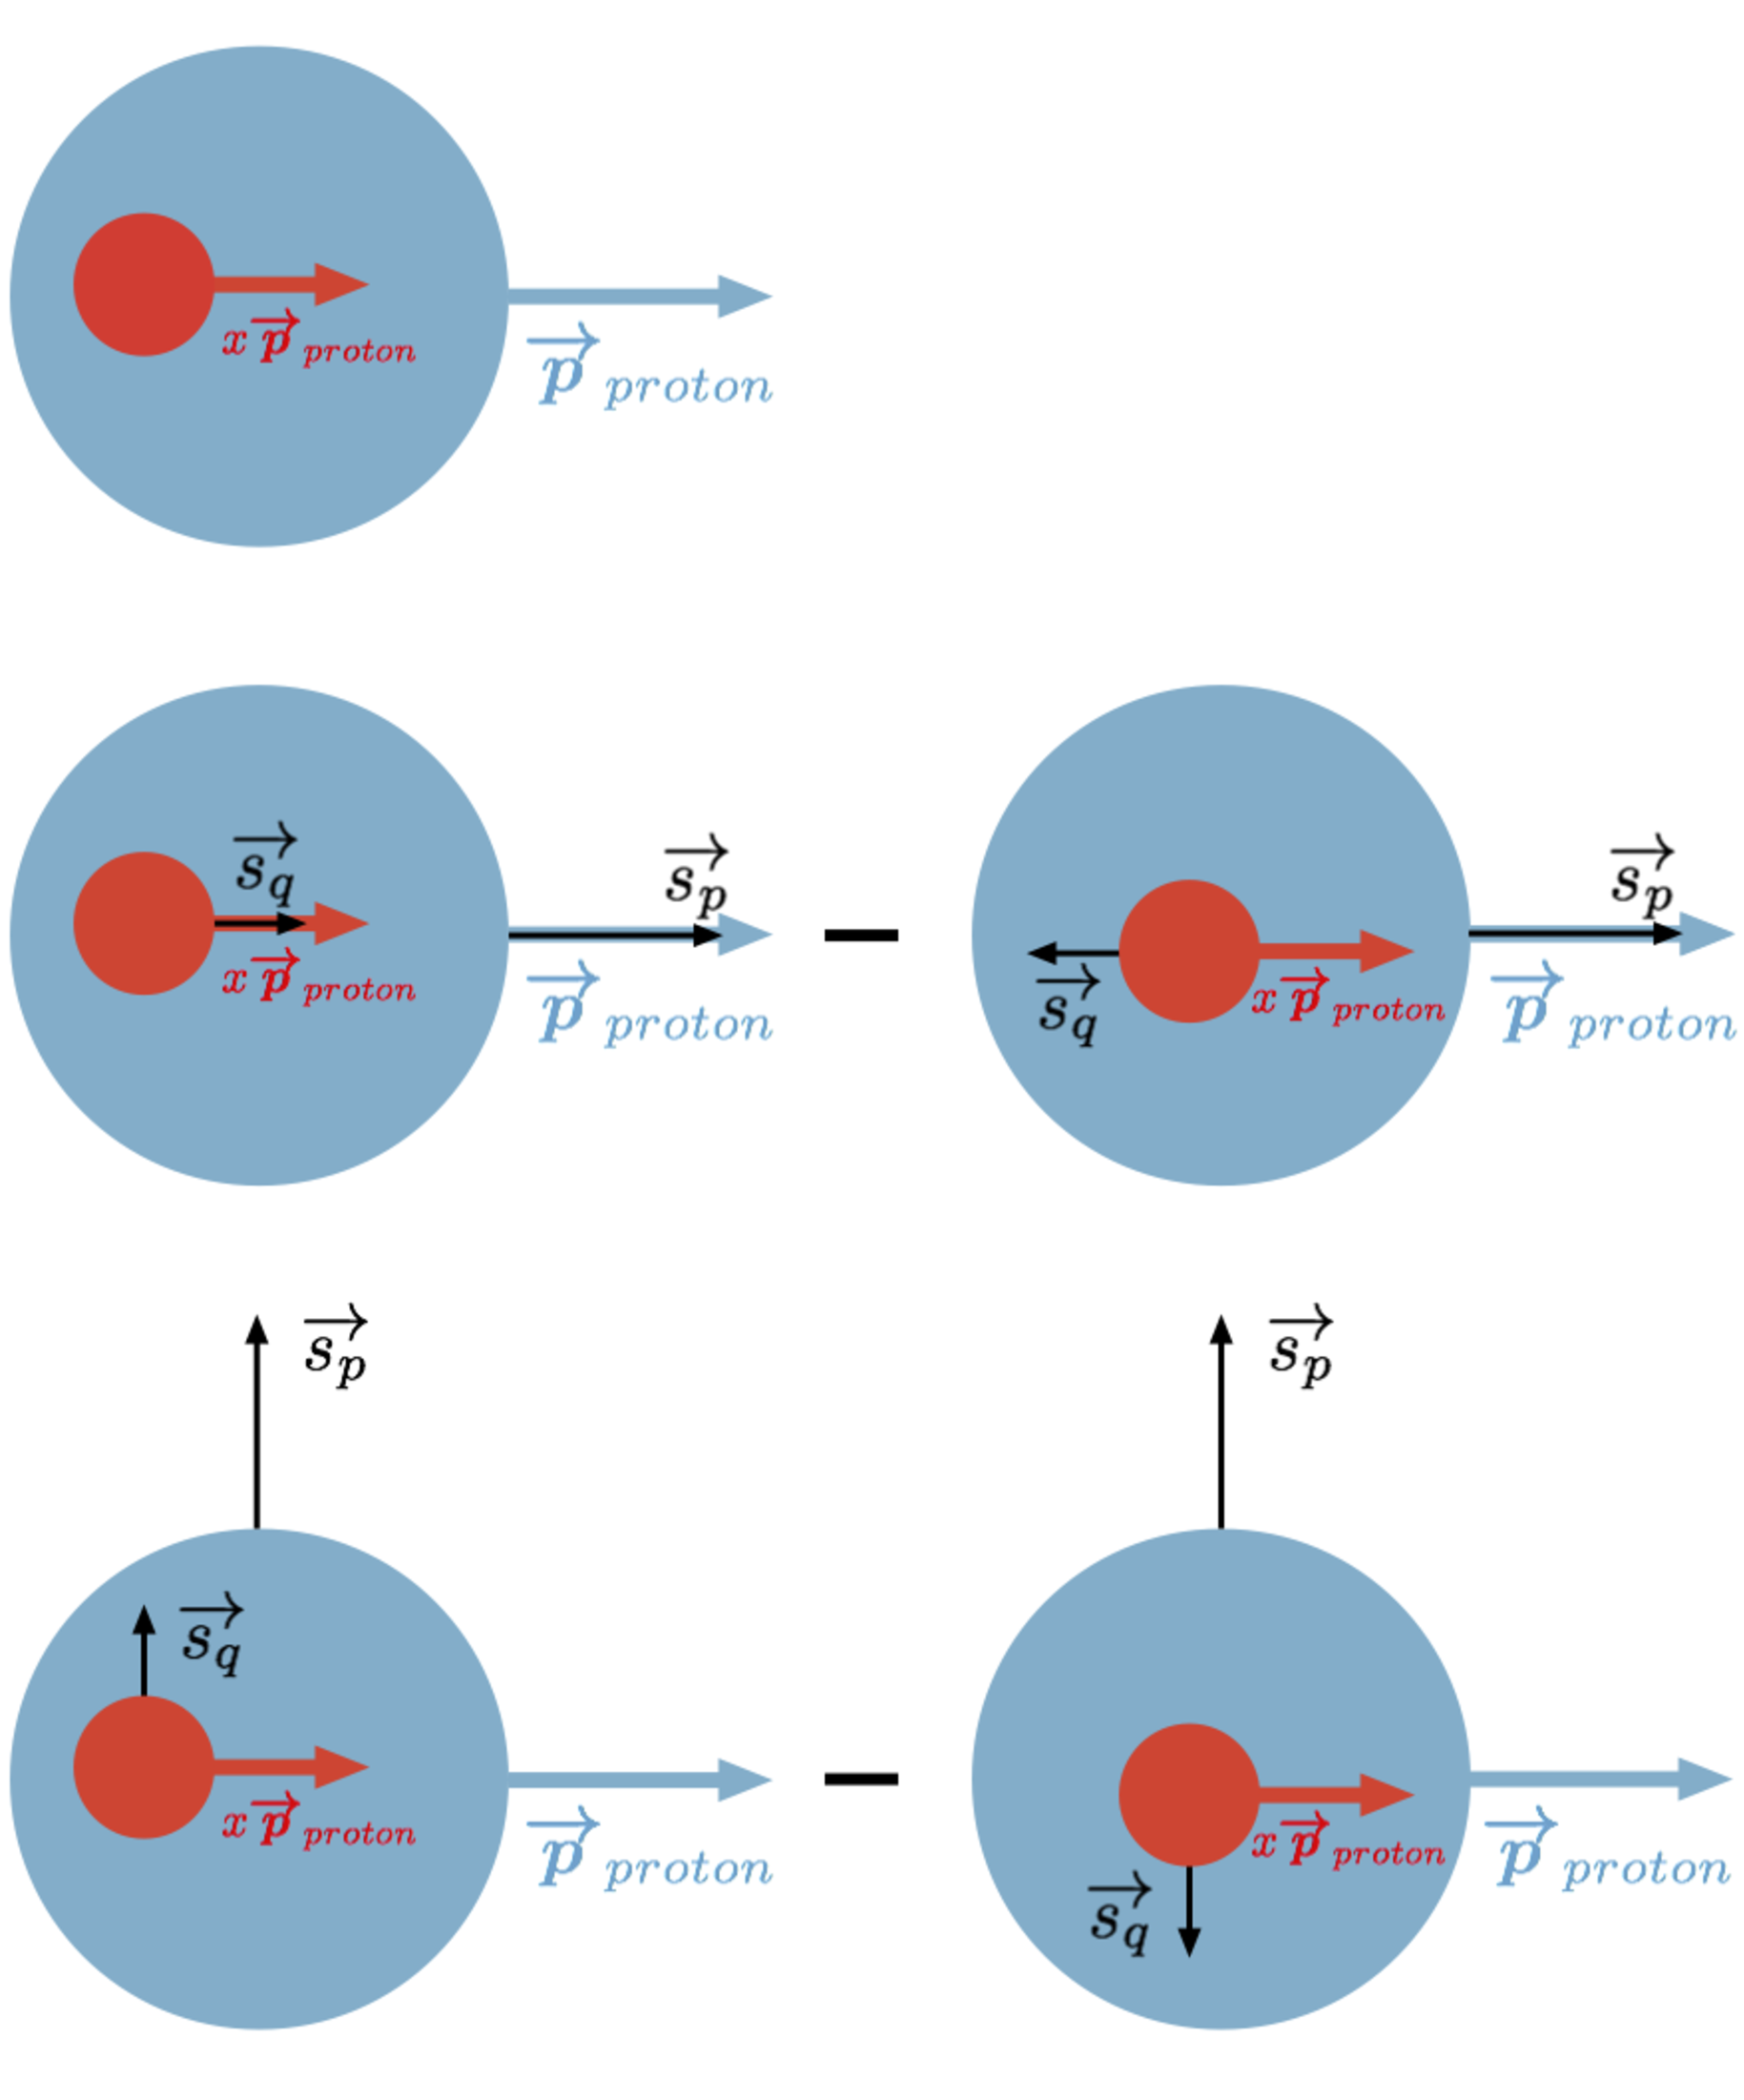
\includegraphics[width = 1\textwidth]{allDistsPic3}
\caption[Visual representation of unpolarized, hellicity, and transversity distribution functions]{Top: Unpolarized distribution function $f_1(x)$ \\
Middle: Helicity distribution function $g_1(x)$ \\
Bottom: Transversity distribution function $h_1(x)$}
\label{fig:PDFs}
\end{center}
\end{figure}


The unpolarized and helicity distributions, which can be seen in figure \ref{pdfDist}, are known accurately for different Bjorken $x$ and momentum transfer of the hard scattering process $Q^2$. On the other hand, the transversity distribution, which can also be seen in figure \ref{pdfDist}, is not well known at all even for just $x$. This is because the transversity distribution function is chiral odd while the unpolarized and helicity distributions are chiral even. This allows the unpolarized and helicity distribution to be accessed through DIS. Since all observables must be chiral even, the transveristy distribution can not be accessed through DIS. It has to be paired with another chiral odd quantity to make a chiral even observable. <??DO I DO SOMETHING HERE SHOWING THAT IT'S CHIRAL ODD WITH SOME PICTURES AND STUFF???> \\ 

\begin{figure}
\begin{center}
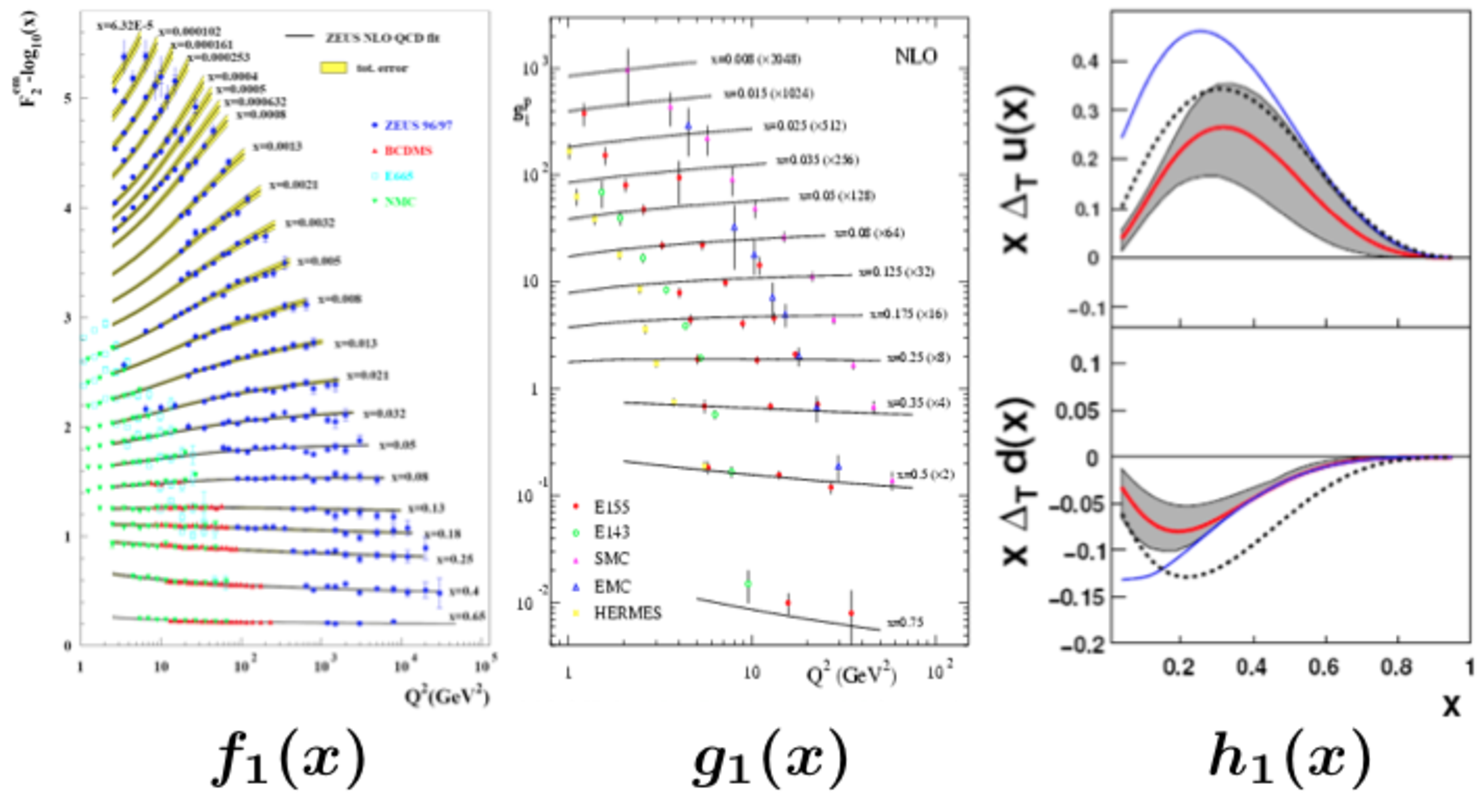
\includegraphics[width = 1\textwidth]{pdfDistributions}
\caption[Current knowlege of parton distribution functions]{Left and center pannels show the unpolarized and helicity distribution functions as a function of momentum transfer $Q^2$ for different values of the momentum fraction $x$. The right pannel shows out best knowlege of the transversity distribution function for the up quark (top) and the down quark (bottom) vs momentum fraction $x$. The grey band shows the uncertainty of the transversity distribution function. The Blue line is a more leanient uncertainty. The dotted line shows the helicity distribution function for the up and down quarks. <ADD REFERENCES TO THE PLOTS>}
\label{fig:pdfDist}
\end{center}
\end{figure}

Several chiral odd candidates to pair with the transversity distribution function have been considered. One such candidate is a transversely polarized Drell-Yan process. This is not ideal because the cross section is small and involves an antiquark transversity distribution as well. <STUFF ABOUT OTHER POSSIBLE CANDIDATES> The candidates which makes the most sense are chiral odd quark fragmentation functions. 


  



\section{Quark Fragmentation}


Quark fragmentation is the .........

We describe the fragmentation process by fragmentation functions. These functions describe how a quark will fragment into the final products we detect. One popular fragmentation function that is connected with the transversity distribution function is the Collins Fragmentation Function .... NEED CITATION HERE ... It describes how a transversly polarized quark fragments into a jet containing a charged pion with momentum $\vec{j}_T$ transverse to the jet axis (Fig \ref{fig:collins}).  

\begin{figure}
\begin{center}
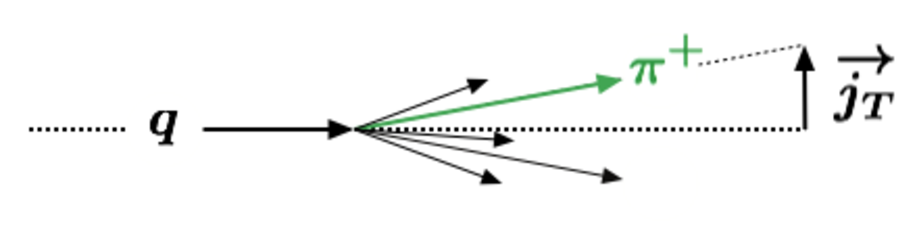
\includegraphics[width = .7\textwidth]{otherFrac2}
\caption[Collins Fragmentation Function]{an outgoing quark fragments into a $\pi^+$ (or $\pi^-$). This is described by the collins fragmentation function. $\vec{j}_T$ is the component of the pion momentum transvers to the jet axis.} 
\label{fig:collins}
\end{center}
\end{figure}


Another way to access transversity is with the Interference Fragmentation Function. This similar fragmentation function to the Collins Fragmentation Function describes the fragmentation of a transversely polarized quart into a pair of oppositely charged pions.    


\begin{figure}
\begin{center}
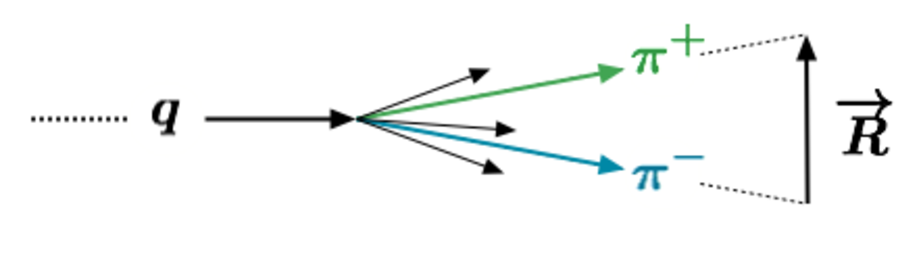
\includegraphics[width = .7\textwidth]{IFFwrite}
\caption[Interference Fragmentation Function]{an outgoing quark fragments into a $\pi^+\pi^-$ pair. This is described by the Interference Fragmentation Function (IFF). The Vector $\vec{R}$ gives the orientation of the pair.}
\label{fig:IFF}
\end{center}
\end{figure}



\chapter{Experimental Landscape}

Before getting into my analysis, I would like to start by acknowledging the experiments that have impacted our knowledge of the parton distribution functions. 

\section{Unpolarized Distribution Function}

\section{The Helicity Distribution Funtion}

The helicity distribution $g_1(x)$ has been measured accurately by multiple collaborations. In 1997 the HERMES collaboration measured the helicity distribution using a combination of inclusive and semi-inclusive lepton-nucleon deep inelastic scattering data. \ref{bib:} The data was taken with 27.6 GeV longitudinally polarized positron beam scattering off a longitudinally polarized hydrogen gas target. They constructed an asymmetry $A_{||}$ in the number of scattered positrons. 

\begin{equation}
A_{||} = \frac{N^-L^+ - N^+L^-}{N^-L_P^+ + N^+L_P^-} 
\end{equation}

Where $N^+(N^-)$ is the number of positrons scattered when the target spin is parallel(antiparallel) to the positron beam spin. The luminosities are $L^+$, $L^-$ when the target spin is parallel or antiparallel with the beam spin, while $L^+_P$, $L^-_P$ are weighted luminosities. The helicity distribution function was extracted based on its relation to this asymmetry.

\begin{equation}
\frac{g_1}{F_1} = \frac{1}{1+\gamma^2}\left[\frac{A_{||}}{D} + (\gamma - \eta)A_2\right]
\end{equation}

   
Hermes is not the only collaboration to extract the helicity distribution. The Hermes data along with other experiments data is shown in figure \ref{fig:helicityDist}. 


 \begin{figure}
\begin{center}
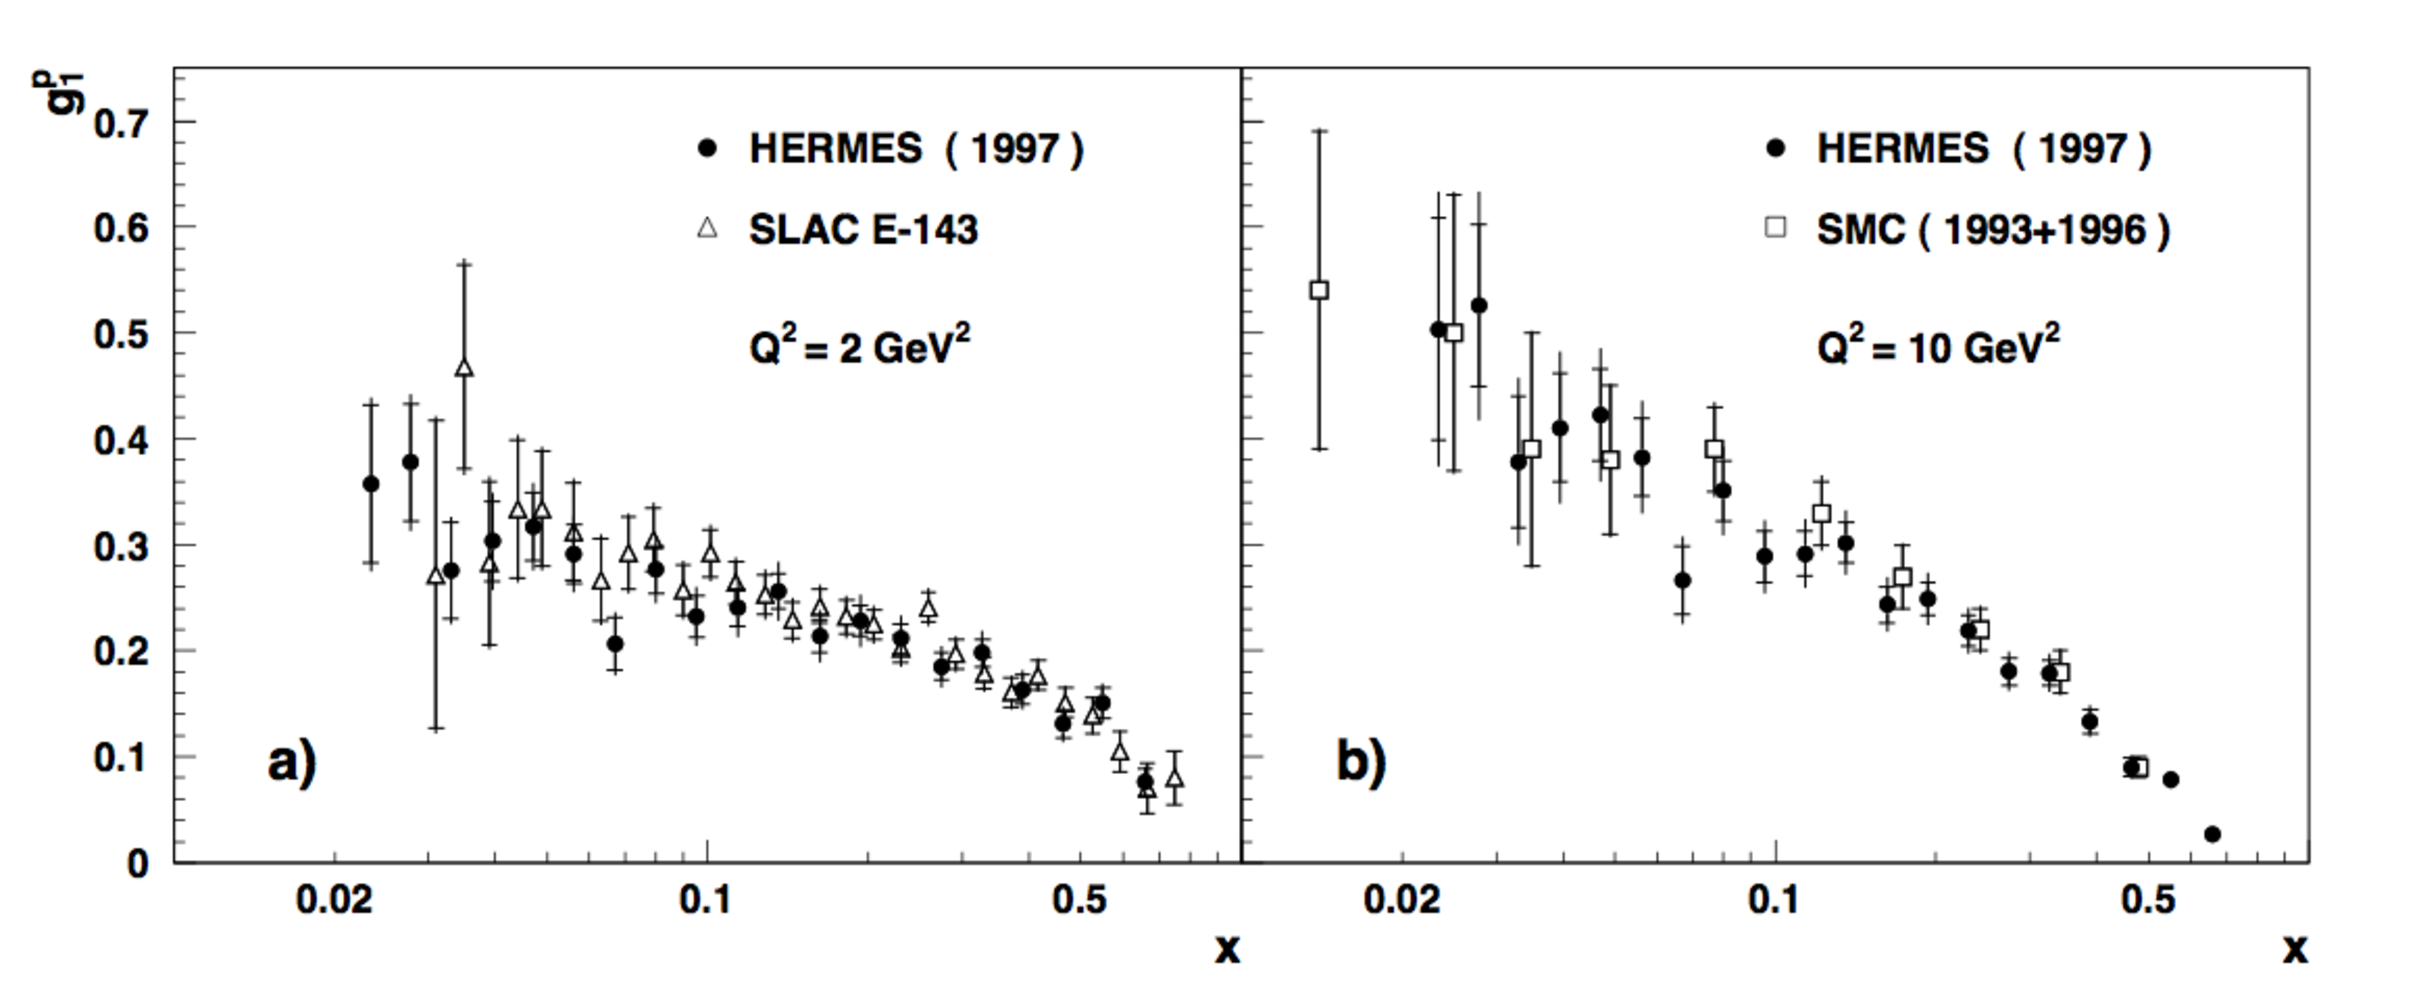
\includegraphics[width = 1\textwidth]{helicityDistFromHermes}
\caption[HERMES results for helicity distribution function]{The helicity distribution as a functuon of momentum fraction x for $Q^2$ = 2 GeV$^2$ and 10 GeV$^2$.}
\label{fig:helicityDist}
\end{center}
\end{figure}

\FloatBarrier
\section{Measuring the Interference Fragmentation Function at Belle}

In our experiment, transversity only shows up as a convolution with the interference fragmentation function $h_1H_1^\sphericalangle$. In order to isolate transversity in our data we need to know how the interference fragmentation function behaves. Luckily for us Belle already did this work. They performed an electron positron annihilation experiment detecting back to back $\pi^+\pi^-$ pairs. A relative angle between the two pions was measured and a modulation $a_{12}$ of the number of back to back pairs found at different values of the relative angle was seen. This modulation is related to two IFFs. 
     
\begin{multline}
%\begin{equation}
a_{12} \propto \frac{1}{2} \frac{\sin^2\theta}{1+\cos^2\theta} \left[ \sum_{q,\bar{q}}e_q^2z_1^2z_2^2H_1^{\sphericalangle q}(z_1, m_1^2)H_1^{\sphericalangle \bar{q}}(z_2, m_2^2)\right] \\ \times \left[ \sum_{q,\bar{q}}e_q^2z_1^2z_2^2D^{q}(z_1, m_1^2)D^{\bar{q}}(z_2, m_2^2)\right]^{-1}
%\end{equation}
\end{multline}

Here $\theta$ is the polar angle defined between the beam axis and the reference axis, $D^q$ is the unpolarized equivalent of the IFF, $z_{1(2)}$ is the energy fraction pion pair 1(2) has, and $m_{1(2)}$ is the invariant mass of pair 1(2). The people at Belle reported the modulation $a_{12}$ for different $z_1,z_2$ bins as well as different $m_1,m_2$ bins for different quark flavors. The modulation $a_{12}$ is shown in figure \ref{fig:BelleMod} plotted versus the invariant mass. With this data, Courtoy et al were able to extract the Interference Fragmentation Function.\cite{extractIFF}

 \begin{figure}
\begin{center}
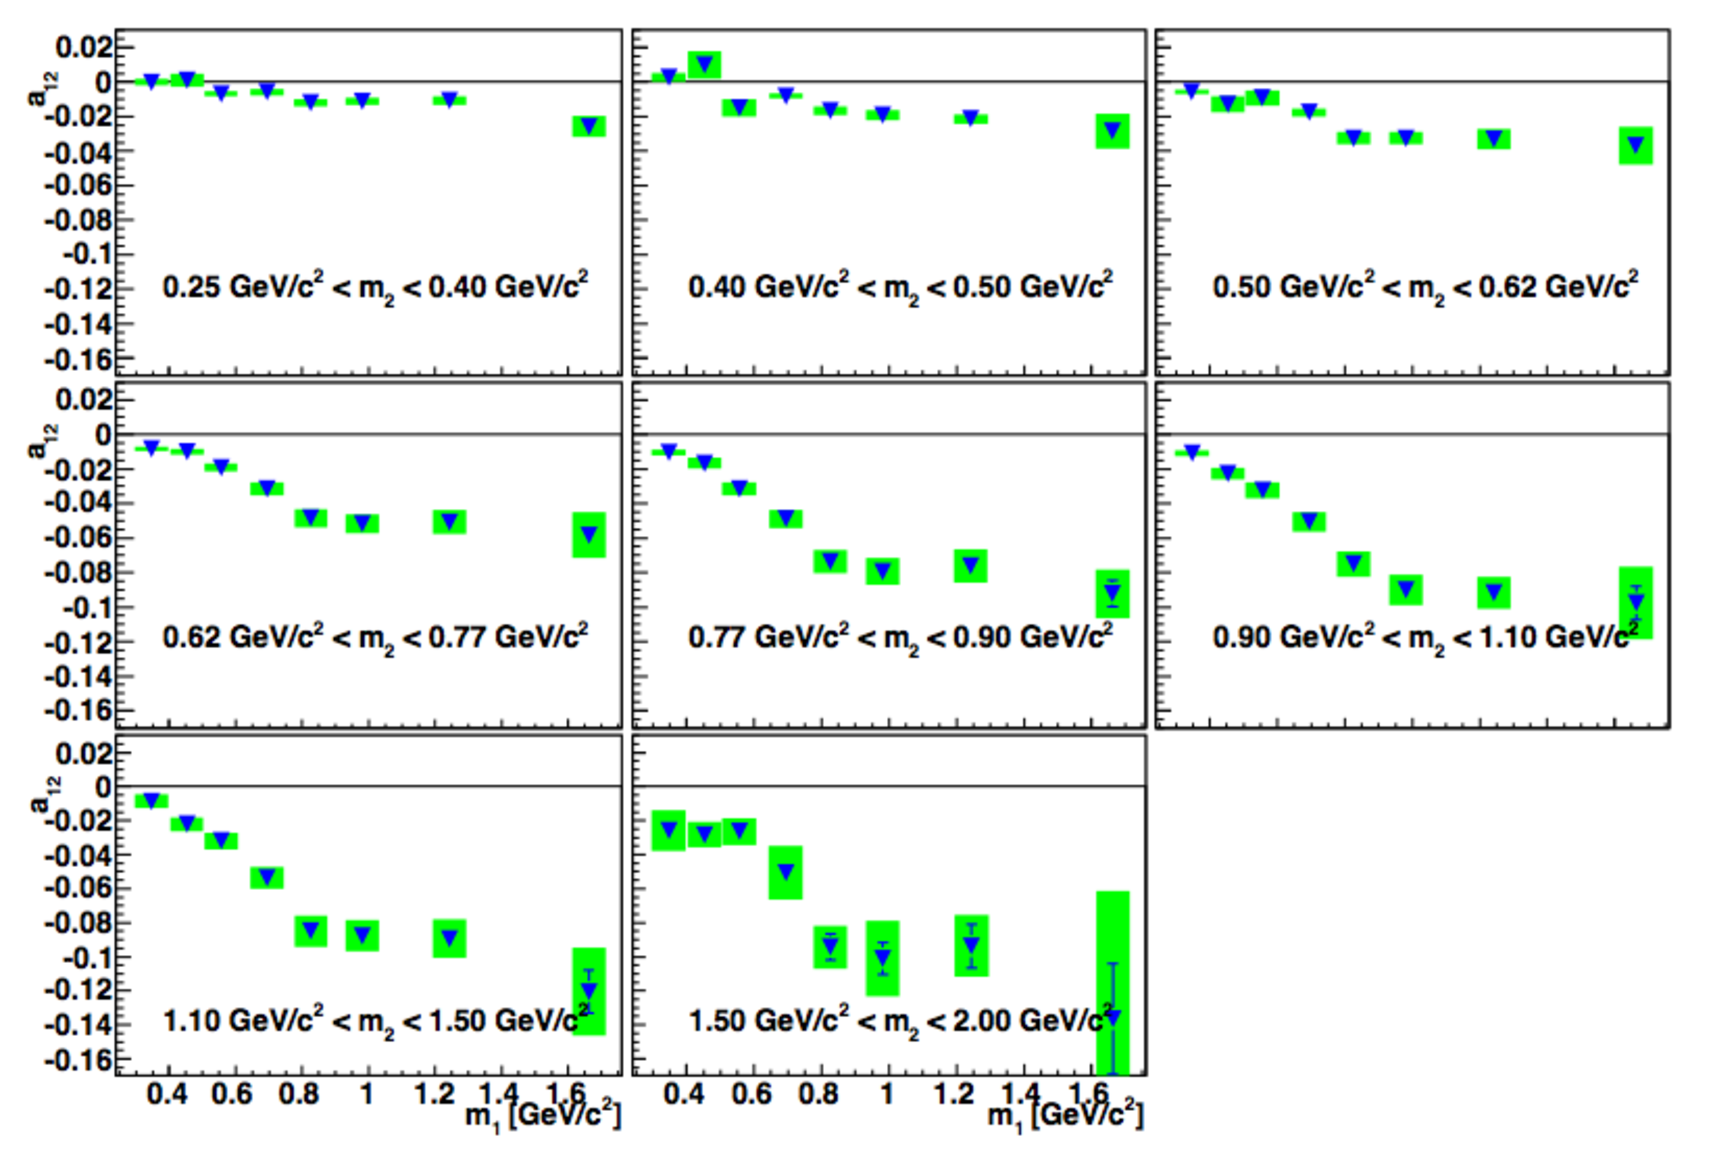
\includegraphics[width = 1\textwidth]{BelleAnnModulationM}
\caption[Asymmetry seen in $e^-e^+$ annihilation at Belle]{Asymmetry in the number of back to back pion pairs seen at Belle plotted vs the invariant mass.}
\label{fig:BelleMod}
\end{center}
\end{figure}

\section{Extracting Transversity}

There have been some experiments 



\chapter{RHIC and The STAR Experiment}

\section{The RHIC complex}
The Relativistic Heavy Ion Collider, located at Brookhaven Nation Lab, is one of the only places in the world that allows for polarized proton collisions, yet is also able to collide heavy nuclei as the name suggests. It actually is composed of a chain of accelerators which boost the energy in steps before finally injecting the particles into the large ring of RHIC. For heavy nuclei are delivered to the Booster Synchrotron where they are accelerated to 95MeV per nucleon. After which they are transfered to the Alternating Gradient Synchrotron (AGS). Here they re-bunched into four bunches and accelerated to 10.8 GeV per nucleon, at which point they are injected into the RHIC ring and accelerated to their final energy. The highest energy RHIC can accommodate for heavy ions is 100 GeV per nucleon. 
The story for protons is a little different. They are injected already spin polarized into the Booster Synchrotron from an older LINAC accelerator. In order to keep the spin polarization for the proton beam, special magnets called Siberian Snakes are used. These magnets flip the proton spin by 180 degrees. From this point they are accelerated in the Booster and AGS before being injected into the RHIC storage ring. Here they are accelerated up to a maximum 250 GeV. 
The RHIC storage ring itself actually consists of two independent rings 3.8 km in circumference. This allows for the collisions of different species. The independent rings intersect at six locations. the STAR detector is located at one such intersection points. $\left[RHIC project overview\right]$

 \begin{figure}
\begin{center}
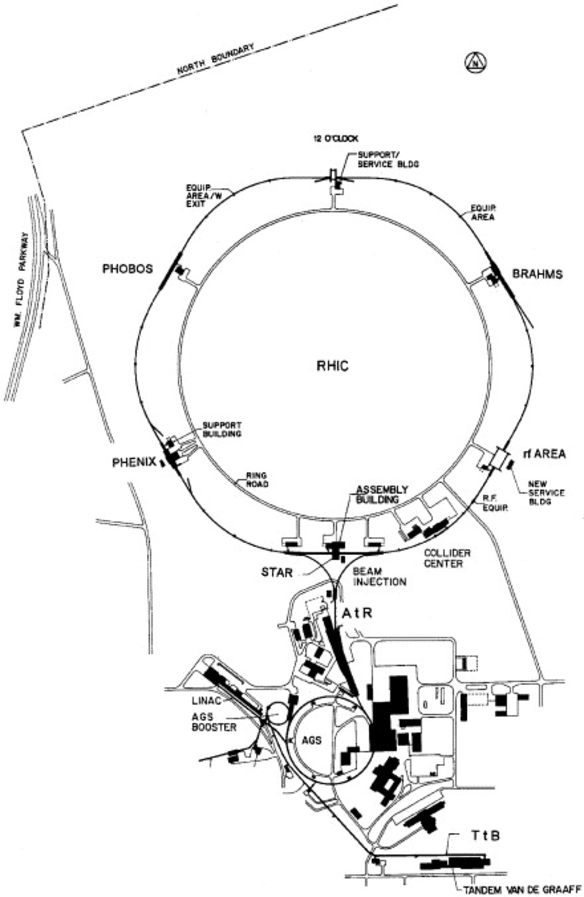
\includegraphics[width = 1\textwidth]{rhicBNL}
\caption[The RHIC complex]{}
\label{fig:rhic}
\end{center}
\end{figure}


As acceleration of polarized protons in a circular accelerator cause resonances which act to depolarize the beam. Special magnets called Siberian Snakes are used to overcome these depolarizing resonances. The roll of the Siberian Snakes rotate the proton spin. If the spin rotation from the Siberian Snakes is much larger than that of the depolarizing resoncances, the beam polarization is kept intact. In the RHIC ring, this is achieved with Siberian Snakes which rotate the proton spin by 180 degrees. The lower energy of the AGS calls for only partial Siberian Snakes which rotate less than 180 degrees, but still enough to maintain beam polarization. \cite{ppCollider}
Each Siberian Snake consists of 4 superconducting helical dipole magnets. Along with the Siberian Snakes, spin rotators are located at the six interaction points. These allow for the proton spin to be rotated from the transverse plane to the longitudinal plane.  \cite{ppCollider}

Polarized protons start out as polarized $H^-$ ions produced from an optically pumped proton ion source (OPPIS).  This source produces $9\times 10^{11}$ polarized $H^-$ ions per 300$\mu$s pulse. These polarized ions are then accelerated to 200 MeV in the LINAC. They are then stripped of the electrons and injected into the Booster where they are further accelerated to 10.5 GeV. From here they are sent to the AGS and accelerated to 25 GeV. The final step is a transfer to RHIC for acceleration to a maximum of 25 GeV and storage.   \cite{ppCollider}
\begin{figure}
\begin{center}
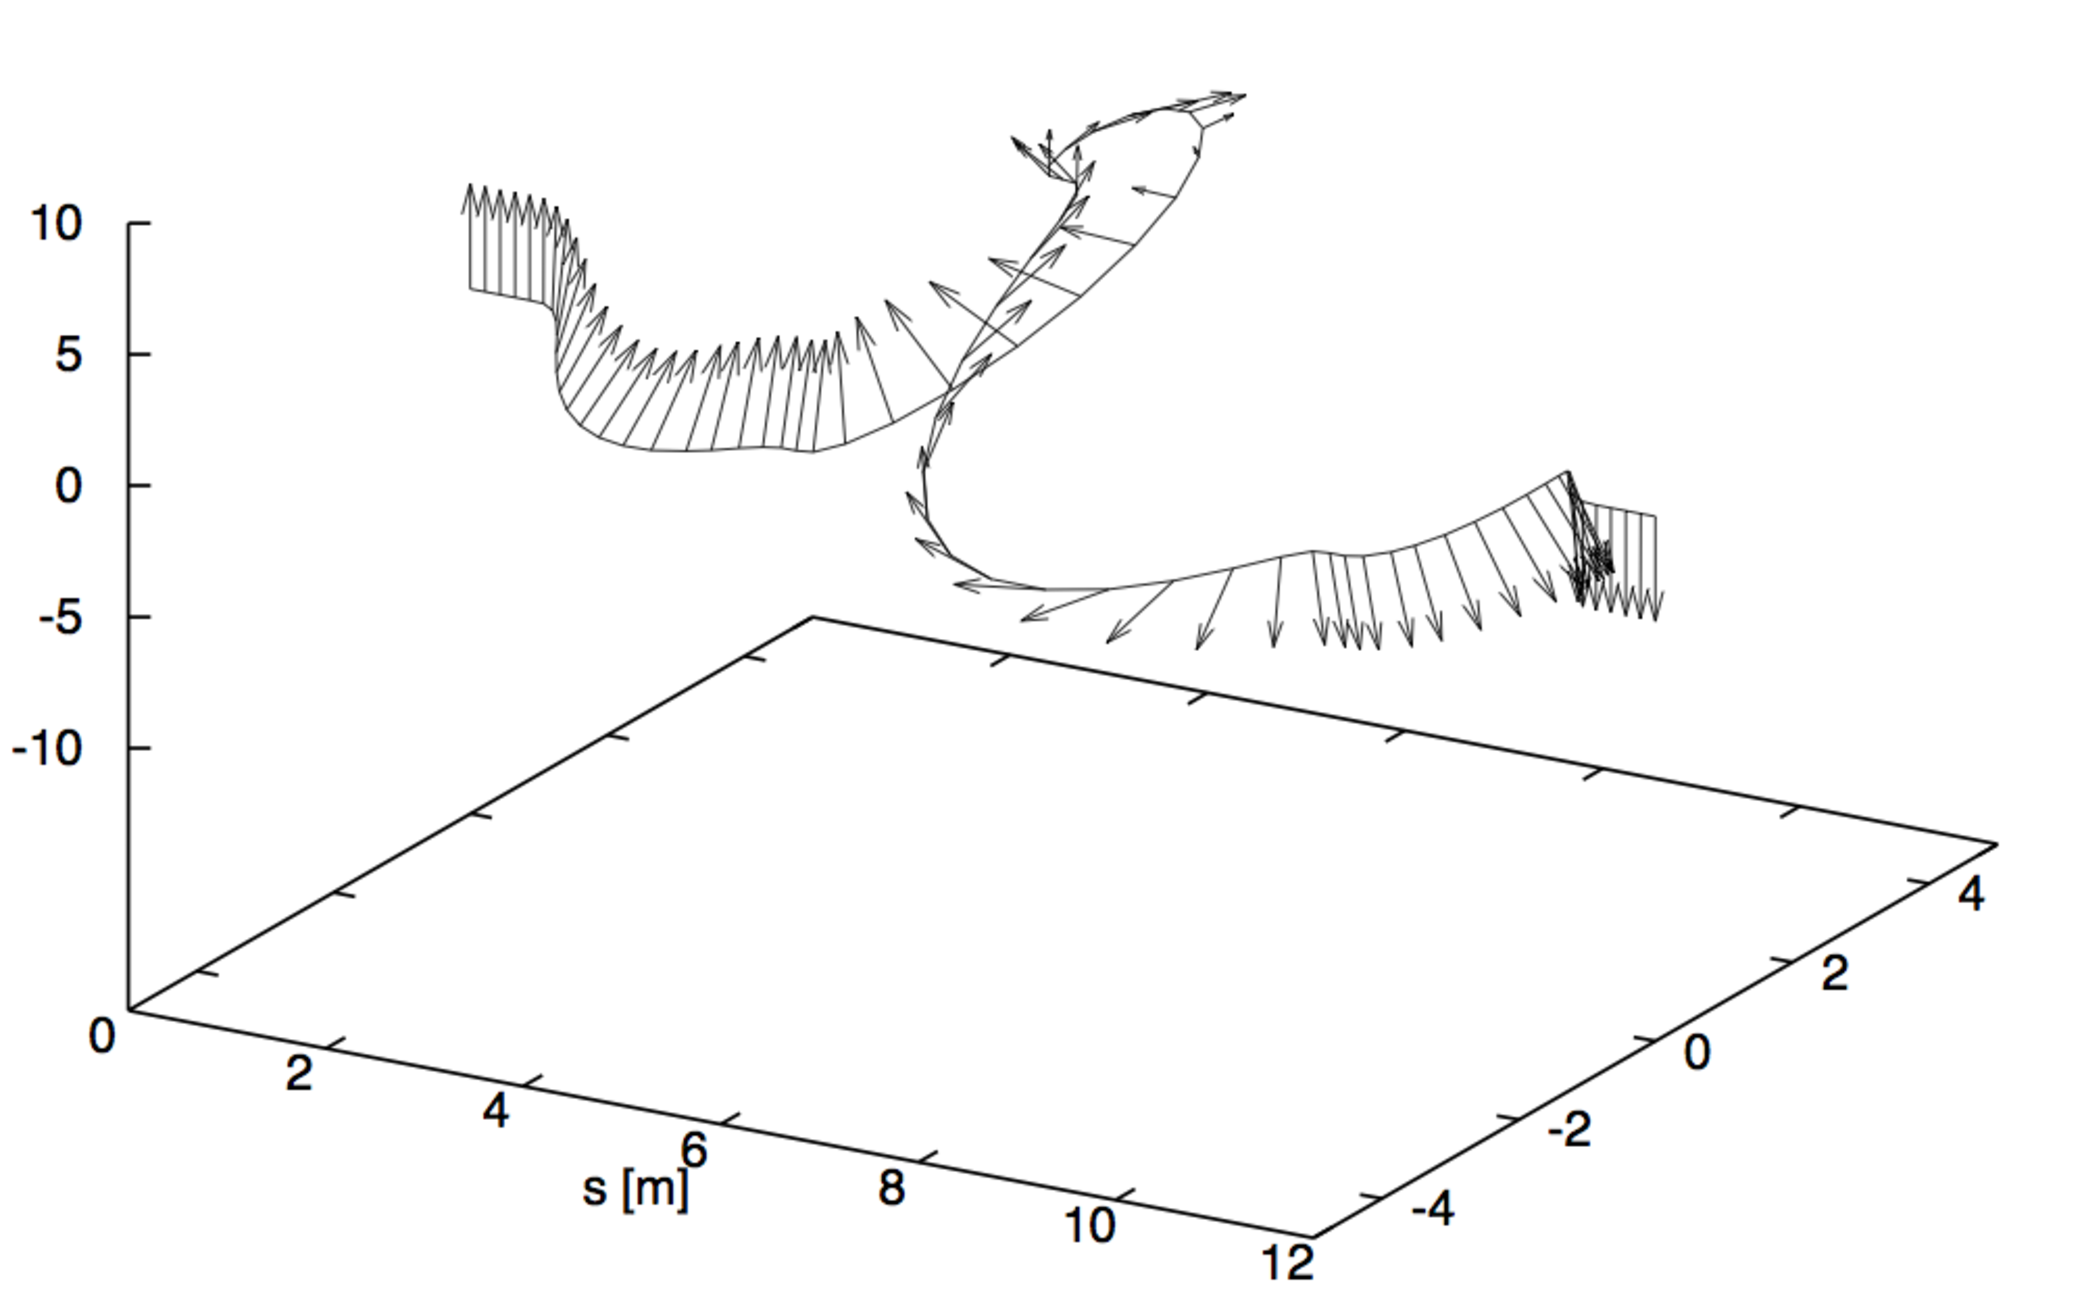
\includegraphics[width = 1\textwidth]{spinFlipFromPaper}
\caption[Spin flip by Siberian Snake]{180 degree proton spin flip by Siberian Snake}
\label{fig:spinFlip}
\end{center}
\end{figure}



\FloatBarrier

\section{The STAR Detector}
The Solinoid Tracker at RHIC (STAR) is bullshit about the history and stuff.

\subsubsection[TPC]{Time Projection Chamber}
One of they key detectors of STAR is the Time Projection Chamber (TPC). It is tasked with tracking particles, measuring momenta, and detecting dE/dx energy loss to aid in particle identification. As a track traverses the TPC it ionizes the gas inside. The track also bends due STAR's magnetic field an amount proportional with the velocity of the track. These allow for the tracking of particles, the measurement of particle momenta, and the dE/dx ionization energy loss aids in particle identification. 

\begin{figure}
\begin{center}
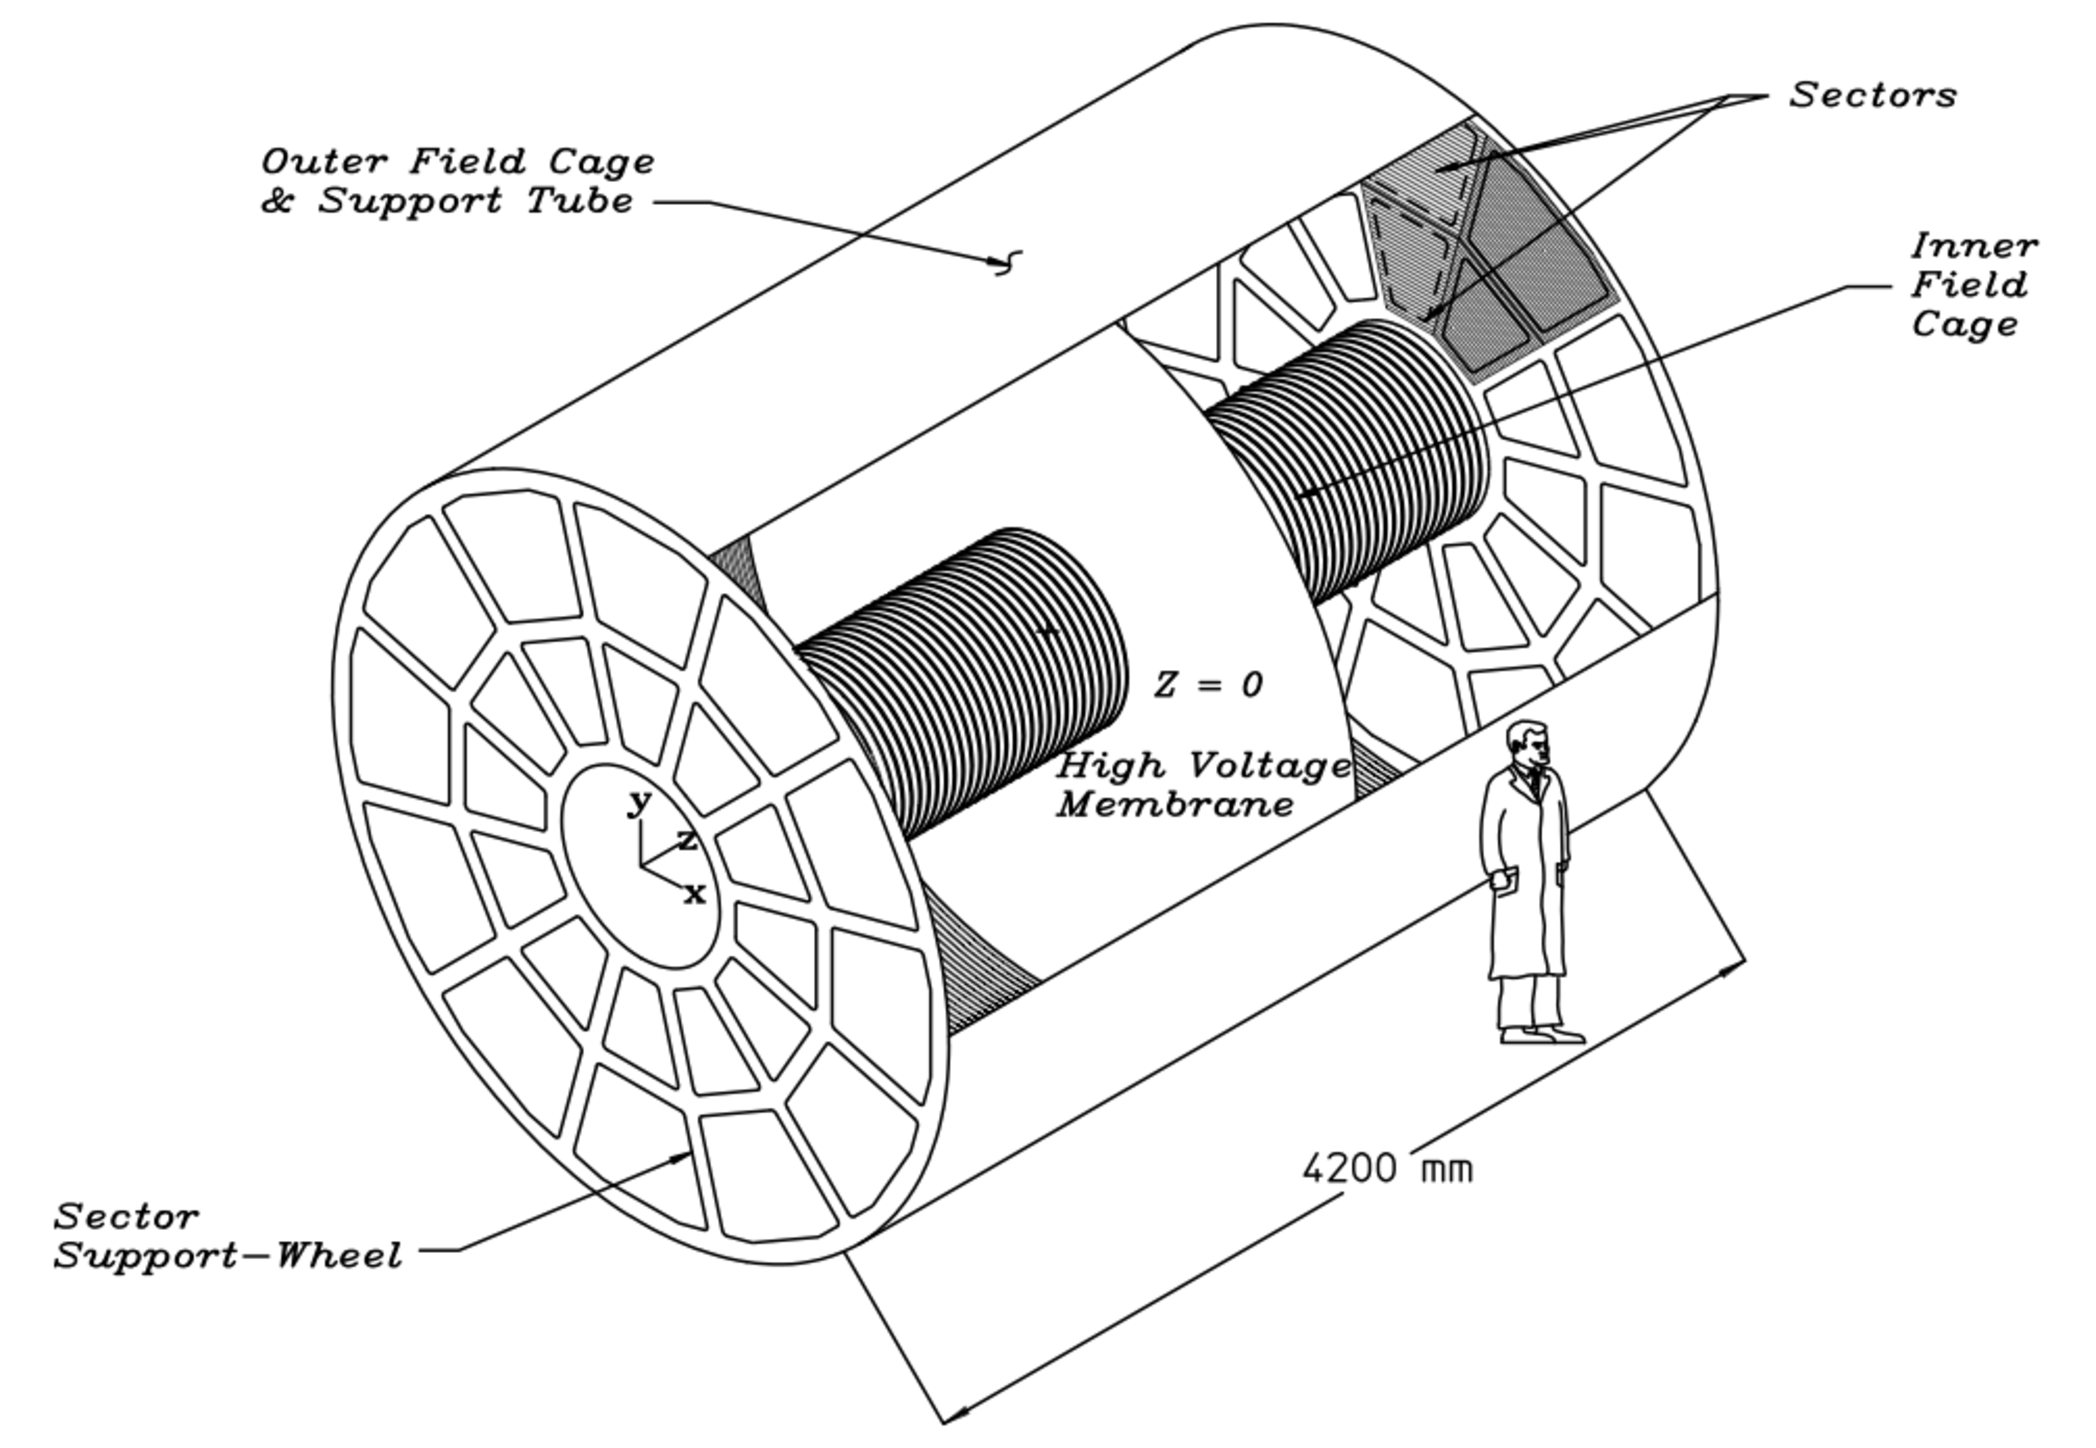
\includegraphics[width = 1\textwidth]{tpcSchem}
\caption[STAR Time Projection Chamber]{STAR Time Projection Chamber}
\label{fig:tpcSchem}
\end{center}
\end{figure}


The TPC is the large cylindrical gas chamber coversing $\pm1.8$ units of pseudorapidity around the interaction point. It's filled with a mixture of 10$\%$ methane and $90\%$ argon at a pressure of 2mbar above atmospheric pressure. As a charged particle passes through the TPC, the gas is ionized. Electrons from the ionization drift to the end caps of the TPC under a uniform electric field of about 135 V/cm where they are reconstructed.

At the center of the TPC is a central membrane which splits the TPC in two halves. This membrane is kept at 28 kV while the two end caps are at ground. A field cage is located around the TPC to create 182 equipotential slices in the TPC. This set up allows for a very uniform electric field to be kept.   

A mixture of 10$\%$ methane and $90\%$ argon is chosen for the TPC gas due to its fast drift velocity. This drift velocity also peaks at the operating electric field (135 V/cm) making it relatively unaffected by subtle fluctuations in the electric field.

The TPC gas drift velocity is calibrated with a laser system. Thirty six aluminum plates are positioned on either side of the central membrane and are illuminated with an ultraviolet laser. This causes photo-ejection of electrons which drift to the end caps where they are read. The position of the aluminum plates are known with such precision that the time it takes the ejected electrons to reach the end cap readouts as well as the position they reach can be used for calibration. 

The end cap is equipped with 12 modular sectors arranged in a circle. These sectors are arrange like a clock with only 3mm separating them. Each sector, shown in figure \ref{fig:tpcPad}, has a grid of readout pads and a wire proportional chamber consisting of three wire girds; a gated grid, a shield (or ground) grid and and anode grid. The gated grid is required to keep boundary conditions with the central membrane and field cage in order to achieve the uniform electric field, and is thus arranged to do so. The anode wire plane is made up of 20$\mu$ wires aligned radially around the sector. This is to achieve maximum precision of the measurement of momenta from high momentum (straight) tracks. The anode grid is completed by wires in the other direction separated by 4 mm.

\begin{figure}
\begin{center}
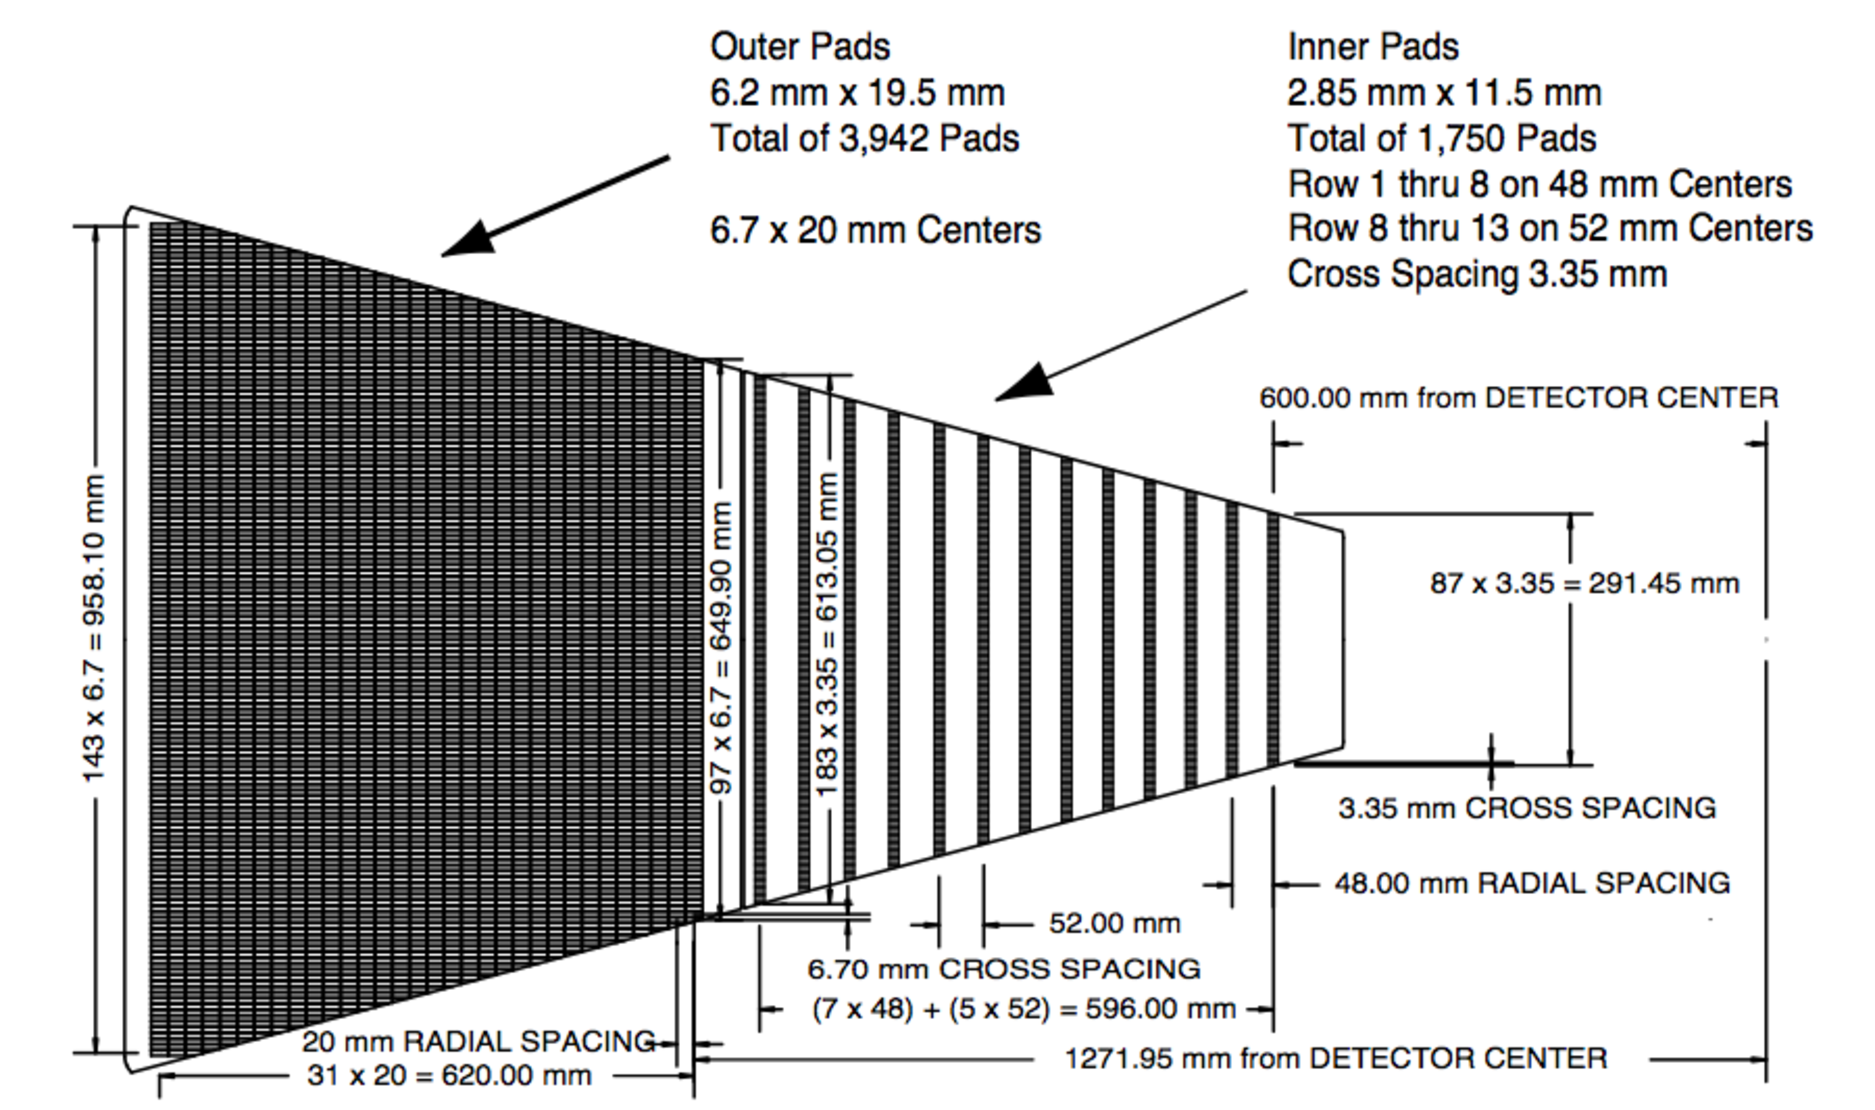
\includegraphics[width = 1\textwidth]{tpcPAD}
\caption[Anode sector of STAR TPC]{One of the 12 anode sectors of the TPC. The outer portion has densly packed pads, while the inner portion is composed of wider rows.}
\label{fig:tpcPad}
\end{center}
\end{figure}


As the drifting electrons reach the anode grid an avalanche occurs triggering a temporary image charge to be induced on the read out pads. The width of each read out pad is chosen such that only three read out pads will share the signal from a single avalanche. This allows for the best centriod reconstruction. The grid of read out pads is broken up into two sections. The outer portion of the grid has continuously packed read-out pads measuring 6.7mm by 20mm optimized for good dE/dx resolution. These pads are located 4mm behind the anode grid. The inner portion has smaller read out pads measuring 3.35 mm by 12 mm optimized for good 2 hit detection. This helps with the large track density seen in the inner portion of the TPC. Unfortunately the available space for electronics for the small pads isn't large enough to have continuous coverage as in the outer section. Instead they are arrange in stripes as seen in figure \ref{fig:tpcPAD}. This arrangement prohibits the inner section to be much help in dE/dx resolution. \cite{TPC}



\begin{figure}
\begin{center}
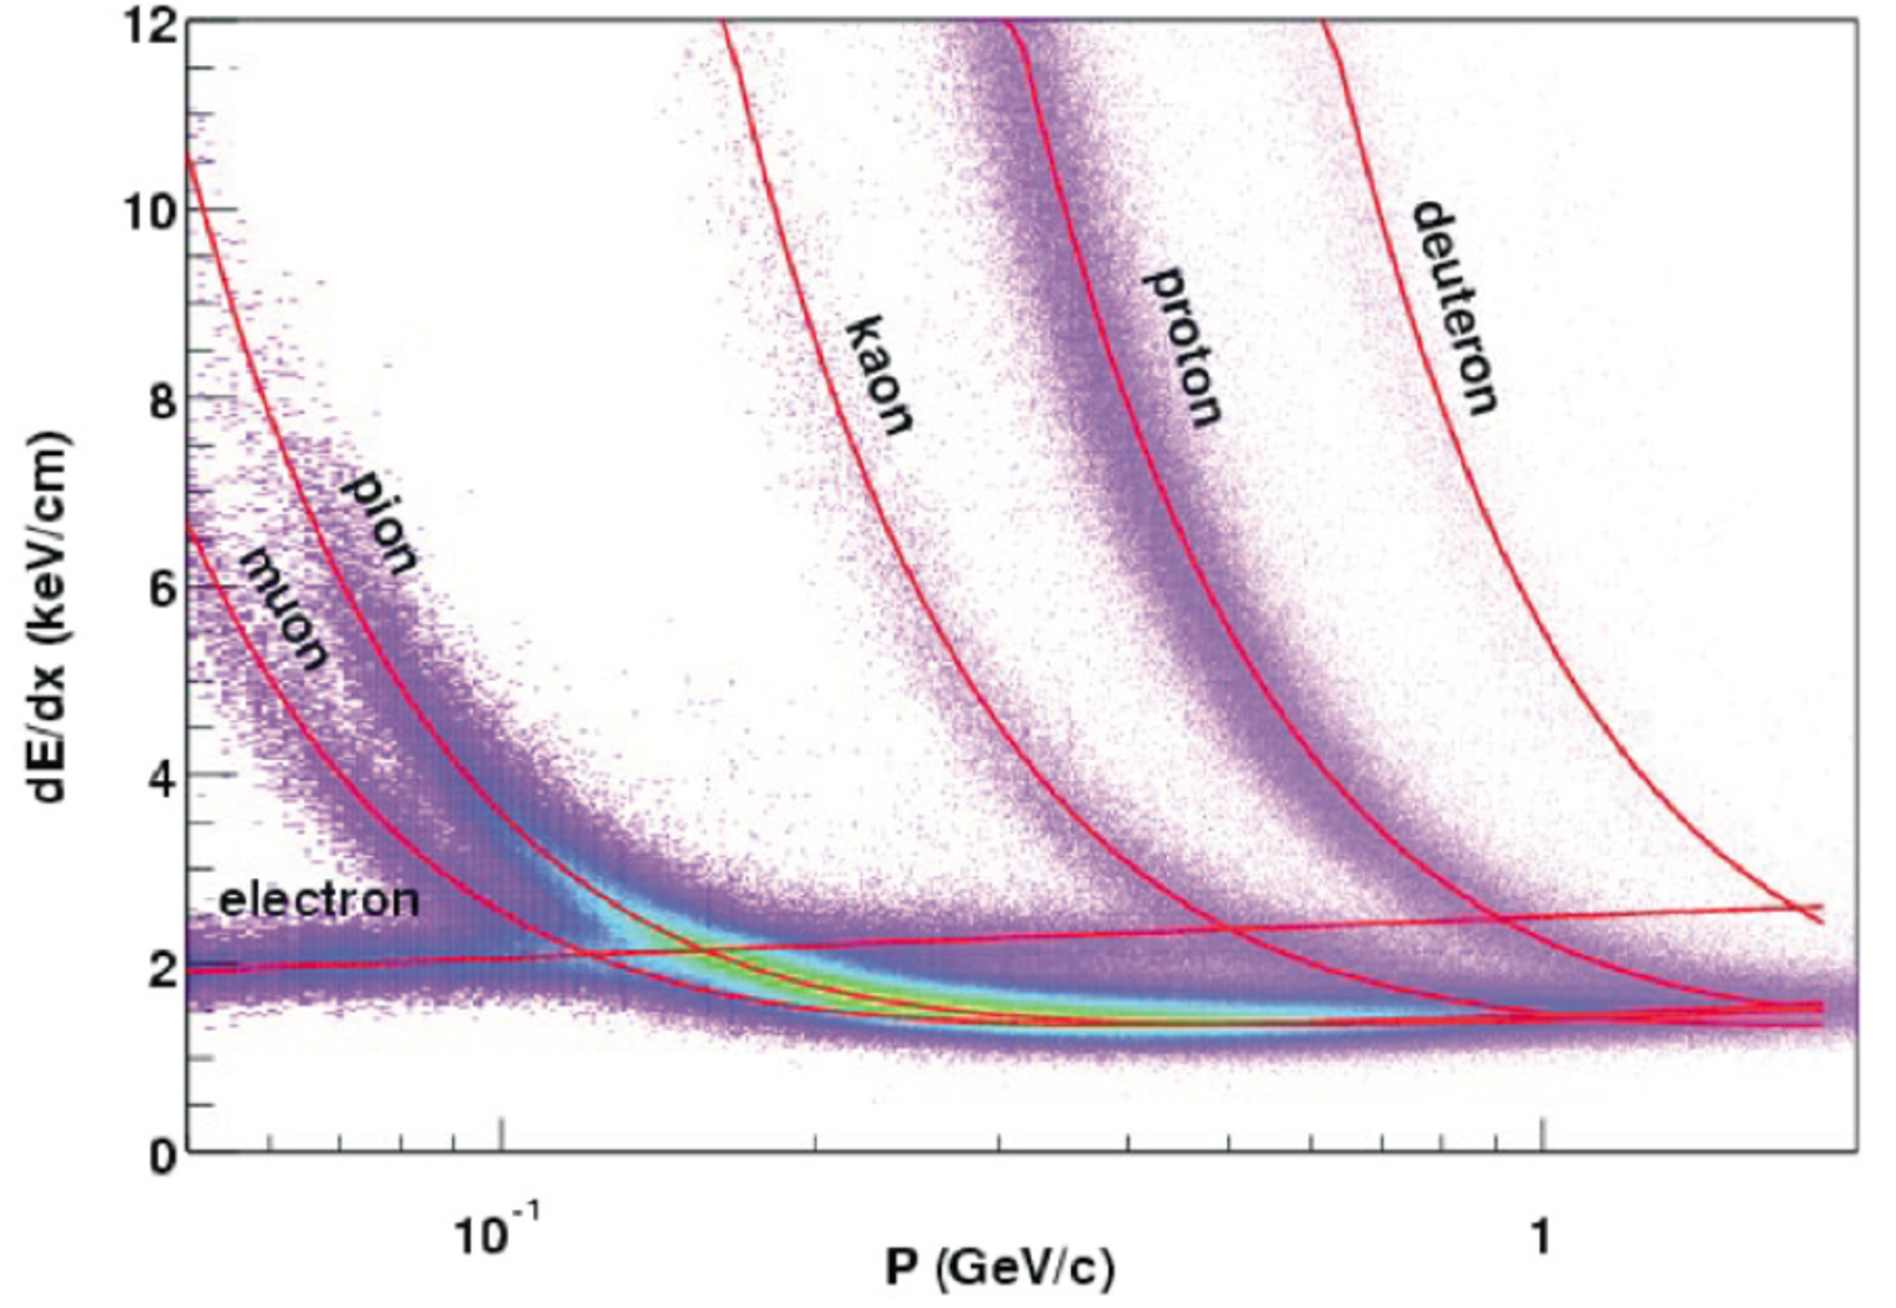
\includegraphics[width = 1\textwidth]{tpc_dEdx}
\caption[Ionization energy loss in TPC gas]{Ionization energy loss in TPC gas. Different species show different energy loss signature. This aids in particle identification.}
\label{fig:tpc_dEdx}
\end{center}
\end{figure}

\FloatBarrier
\subsubsection[BEMC]{Barrel Electromagnetic Calorimeter}

The Barrel Electromagnetic Calorimeter (BEMC) is a large array of lead and plastic scintillator sitting outside the TPC and inside the STAR magnet. At $\eta = 0$ the BEMC is roughly 20 radiation lengths thick allowing it to contain electromagnetic showers up to 60 GeV. Scintillation light is carried from the BEMC array to outside the STAR magnet where it is fed into photomultiplier tubes (PMT).

The BEMC is composed of a total of 4800 towers, each one subtending 0.05$^\circ$ in $\phi$ and 0.05 units in $\eta$. A tower consists of 20 layers of 5 mm thick lead, 19 layers of 5mm thick scintillator, and two layers of 6 mm thick scintillator. Each tower is angled toward the reaction region as seen in figure \ref{fig:BEMC2}.  

The BEMC is equipped with a pre-shower detector which provide readings of the longitudinal shower development after 1 to 1 and a half radiation lengths. Made up of the first two (6 mm) scintillating layers of the tower, the pre-shower detector aids in distinguishing between $\pi^0$ and $\gamma$ as well as between electrons and hadrons. Electrons will typically have a larger ionization energy loss dE/dx inside the BEMC than hadrons resulting in roughly 63\% of electrons showering before the pre-shower volume and 84\% by the middle of the pre-shower detector compared to only 3\% and 6\% for hadrons. The pre-shower detector consists of two 6 mm thick layers of scintillator instead of the 5 mm thick scintillator layers in the rest of the BEMC. 

The active scintillating layers, both pre-shower and regular, are made of Kuraray SCSN81 and light from each layer is carried out with wavelength shifting fiber embedding into the scintillator layer. The scintillation light from each layer is transferred to a 2.1 m long optical cable which carries it passed the magnet to a decoder box. Here the light from all 21 layers in a tower, including the two pre-shower layers, are combined and fed into a single PMT. The pre-shower detector also passes a second sample of scintillation light from layers 1 and 2 to a separate PMT, this time not combined with light from any other layers.  

\begin{figure}
\begin{center}
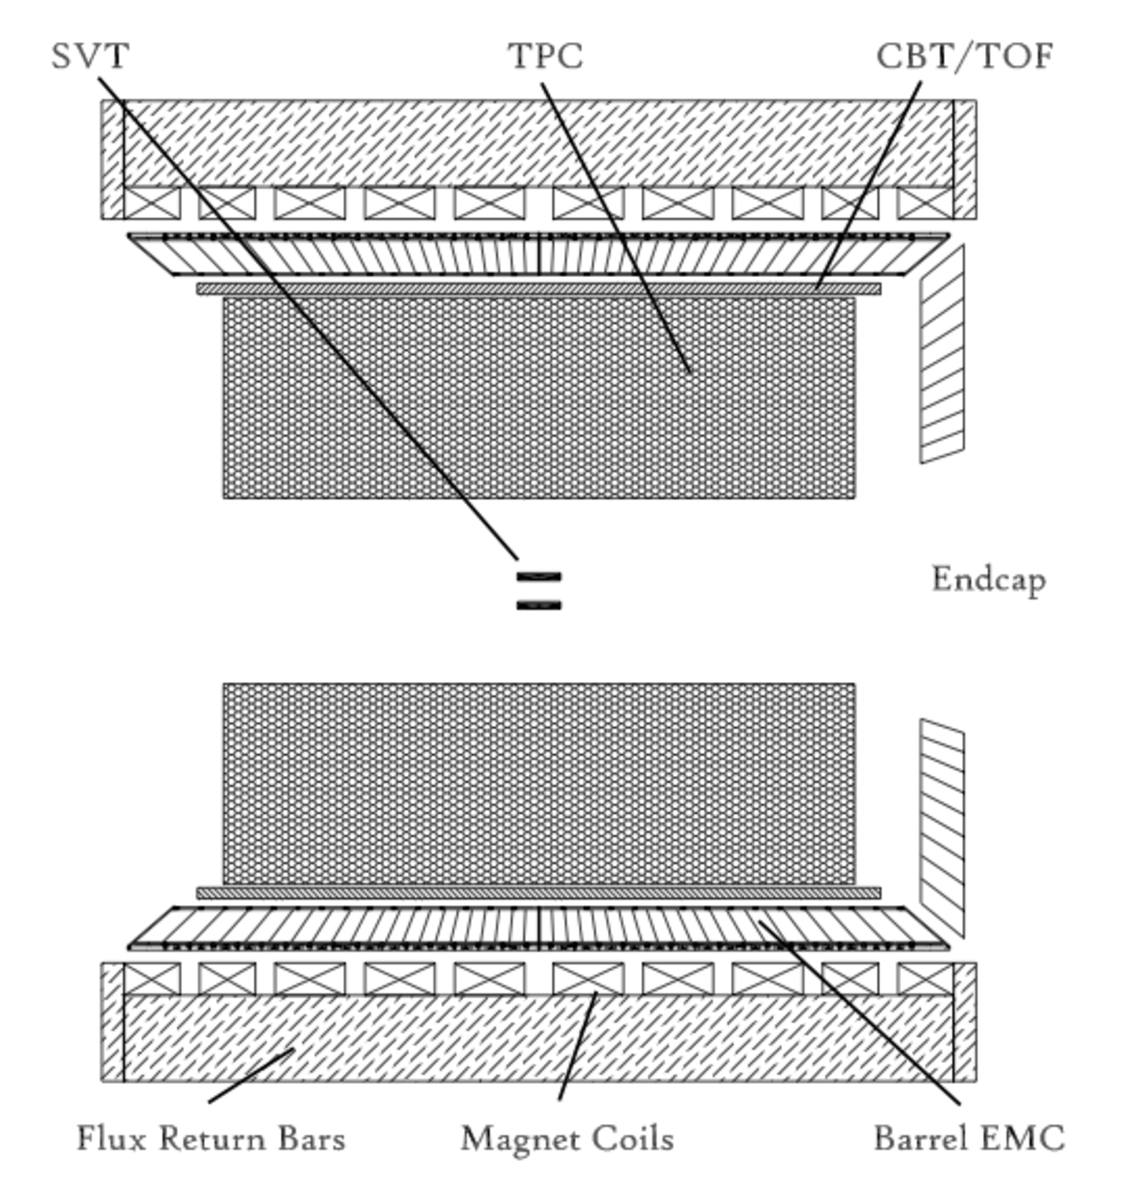
\includegraphics[width = .7\textwidth]{BEMC1}
\caption[Barrel Electromagnetic Calorimeter]{The BEMC is located outside the TPC but inside the STAR magnet and return bars. The scintilation light is transported past the magnet and return bars where it is read out by PMTs.}
\label{fig:BEMC1}
\end{center}
\end{figure}


\begin{figure}
\begin{center}
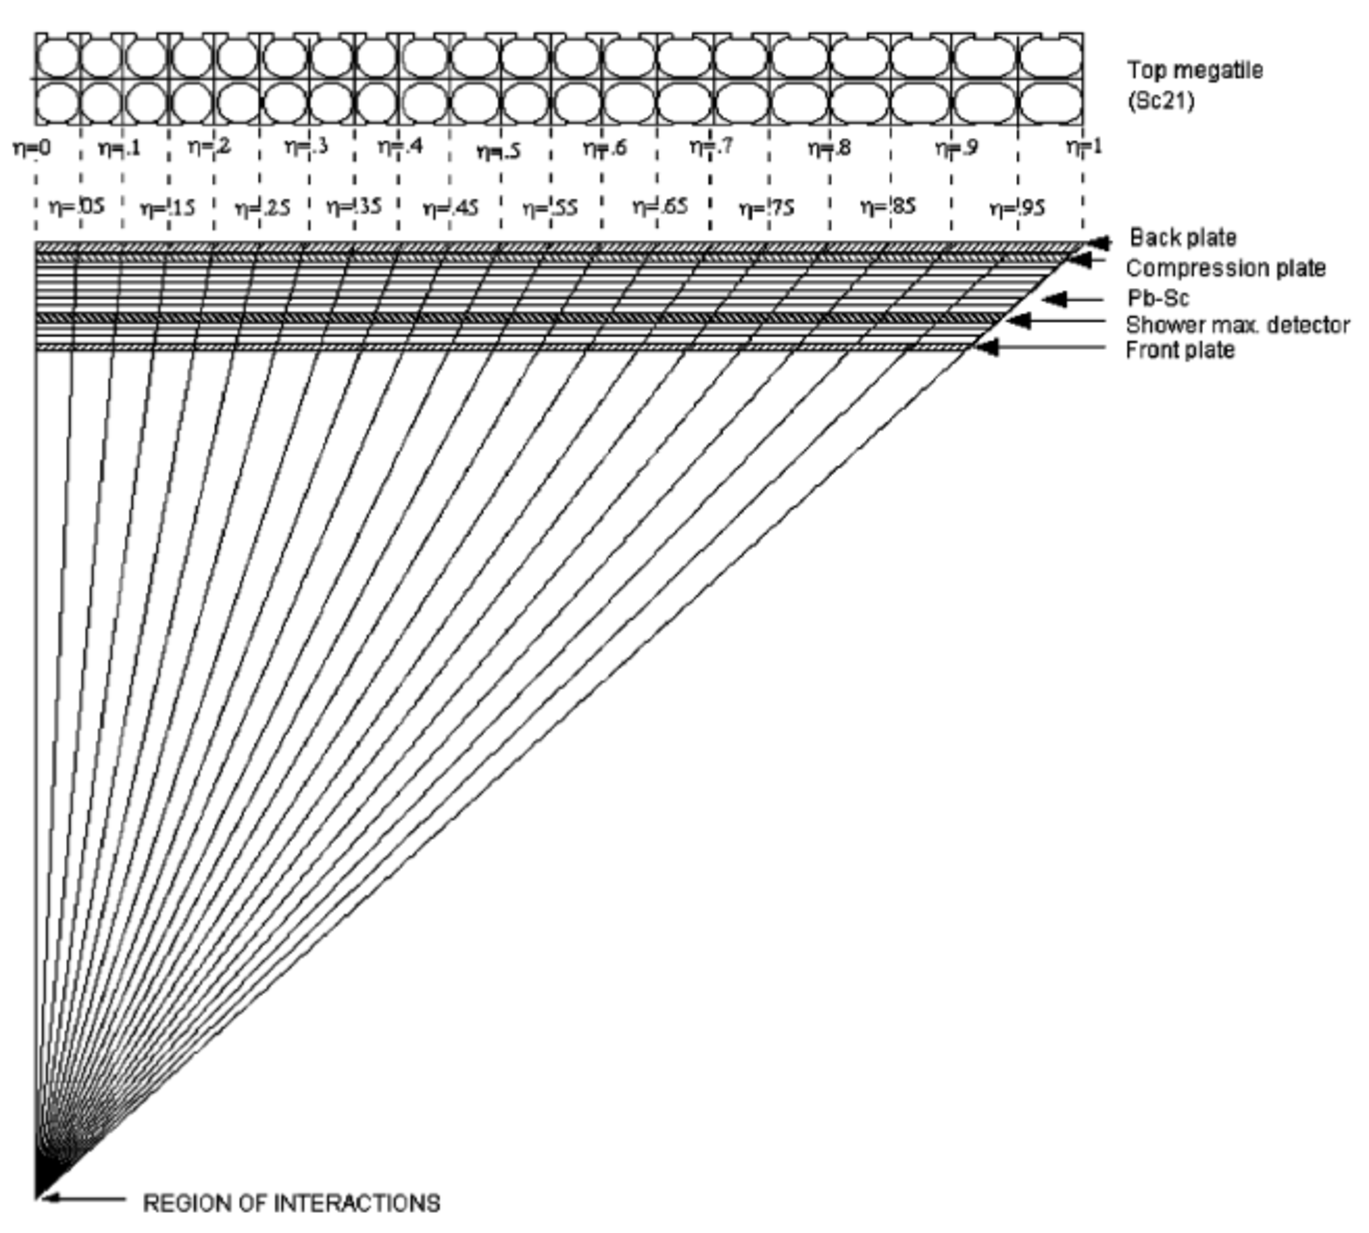
\includegraphics[width = .7\textwidth]{BEMC2}
\caption[Barrel Electromagnetic Calorimeter 2]{Each tower of the BEMC is angled to point back to the interaction region of STAR. The shower max detector as well as the individual scintillator/lead layers are shown.}
\label{fig:BEMC2}
\end{center}
\end{figure}

As neutral particles, such as $\pi^0$, do not ionize the TPC gas, the BEMC is tasked with providing spacial resolution of such species. Instead of making size of each tower of the BEMC comparable to the Moliere radius in the lead, plastic scintillator a shower maximum detector (SMD) is added into the BEMC. The SMD, set at about 5.6 radiation lengths at $\eta=0$, is composed of an aluminum plate with divots on either side. As seen in figure \ref{fig:SMD2}, a 50$\mu$m gold-plated tungsten anode wire lies in each divot. The wires run along the barrel. As the electromagnetic shower passes these wires a charge is induced. This charge is amplified by the gas in the divot. Detection strips are located on the top and bottom faces of the aluminum plate. One set of strips runs parallel to the wires and provides the spacial distribution of the shower in the $\eta$ direction. The other set, running perpendicular to the wires provides the spacial distribution in the $\phi$ direction. A schematic of this is shown in figure \ref{fig:SMD2}. Together They give a full description of the shower position.\cite{BEMC}

\begin{figure}
\begin{center}
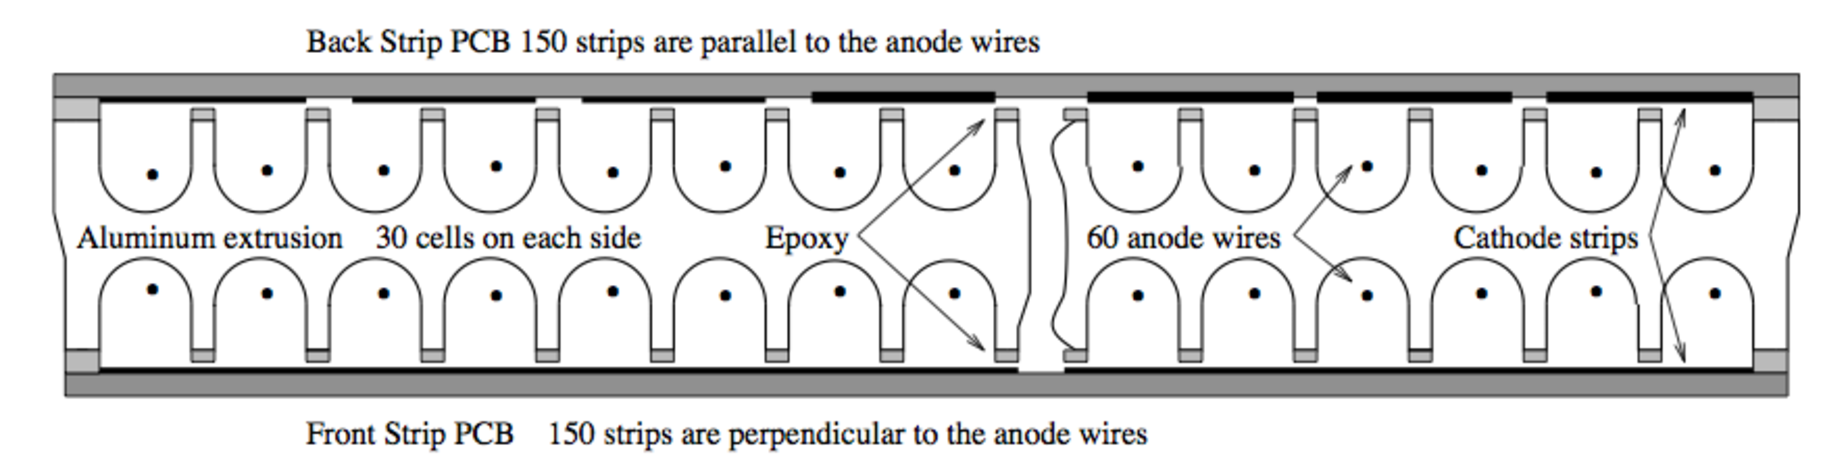
\includegraphics[width = .6\textwidth]{SMD2}
\caption[Shower Maximum Detector cross sectional view]{Cross sectional view of the shower max detector. Aluminum extrusion in the center containing two sets of anode wires. Cathode strips on the top and bottom face run either parralell or perpendicular to the anode wires.}
\label{fig:SMD1}
\end{center}
\end{figure}


\begin{figure}
\begin{center}
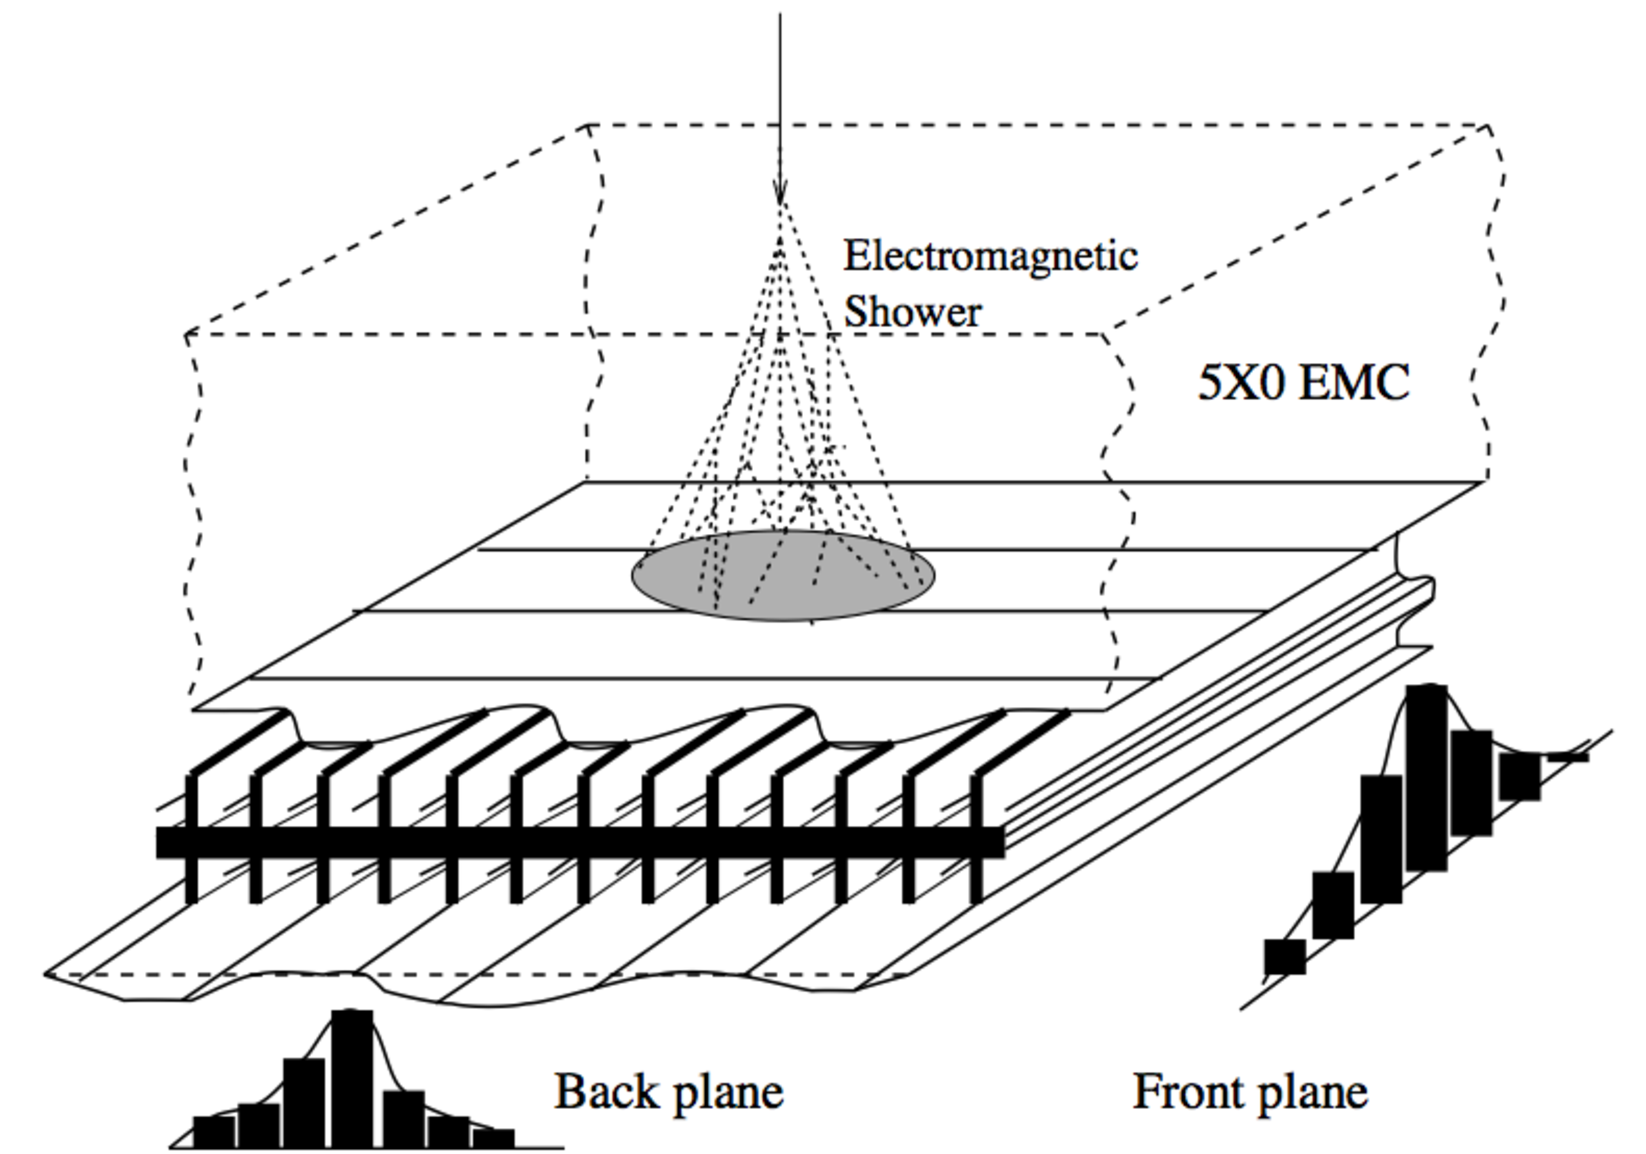
\includegraphics[width = .6\textwidth]{SMD1}
\caption[Spatial reconstruction in the SMD]{Schematic of spatial reconstruction in SMD. The cathode strips on the top and bottom faces read the induced charged in the $\phi$ and $\eta$ directions seperately.}
\label{fig:SMD1}
\end{center}
\end{figure}




\FloatBarrier
\subsubsection[EEMC]{Endcap Electromagnetic Calorimeter}

\subsubsection[TOF]{Time of Flight}

To aid in particle identification STAR has a time of flight system. The system is composed of two different detectors, the Time of Flight Patch (TOFp) and the Pseudo Vertex Position Detector (pVPD).  Together these detectors allow for direct 2$\sigma$ $\pi$/$K$/$p$ identification for track momenta up to about 1.7 GeV/$c$.

The pVPD is responsible for starting the clock of the time of flight system. It consists of two plastic scintillator detectors, one on either side of the STAR interaction region sitting 5.6 m away from the center of the STAR detector. Both are positioned very close to the beam pipe and detect very forward, high energy photons produced in the collision. The average of the time for both detectors to see this photon pulse is declared the "start time" for the event. The scintillation light is read out by PMTs. The magnetic field strength near the pVPD is on the order of a few hundred Gauss. Because of this the PMTs are shielded on the sides with a steel outer shield, a nickel-Iron alloy intermediate shield, and finally a foil inner shield. They are also shielded from the front with a lead face sheet and a steel cap. A pVPD detector element is shown in figure \ref{fig:vpdDetector}. This is mounted to the beam pipe support structure as shown in figure \ref{fig:vpdAssembly}.    

\begin{figure}
\begin{center}
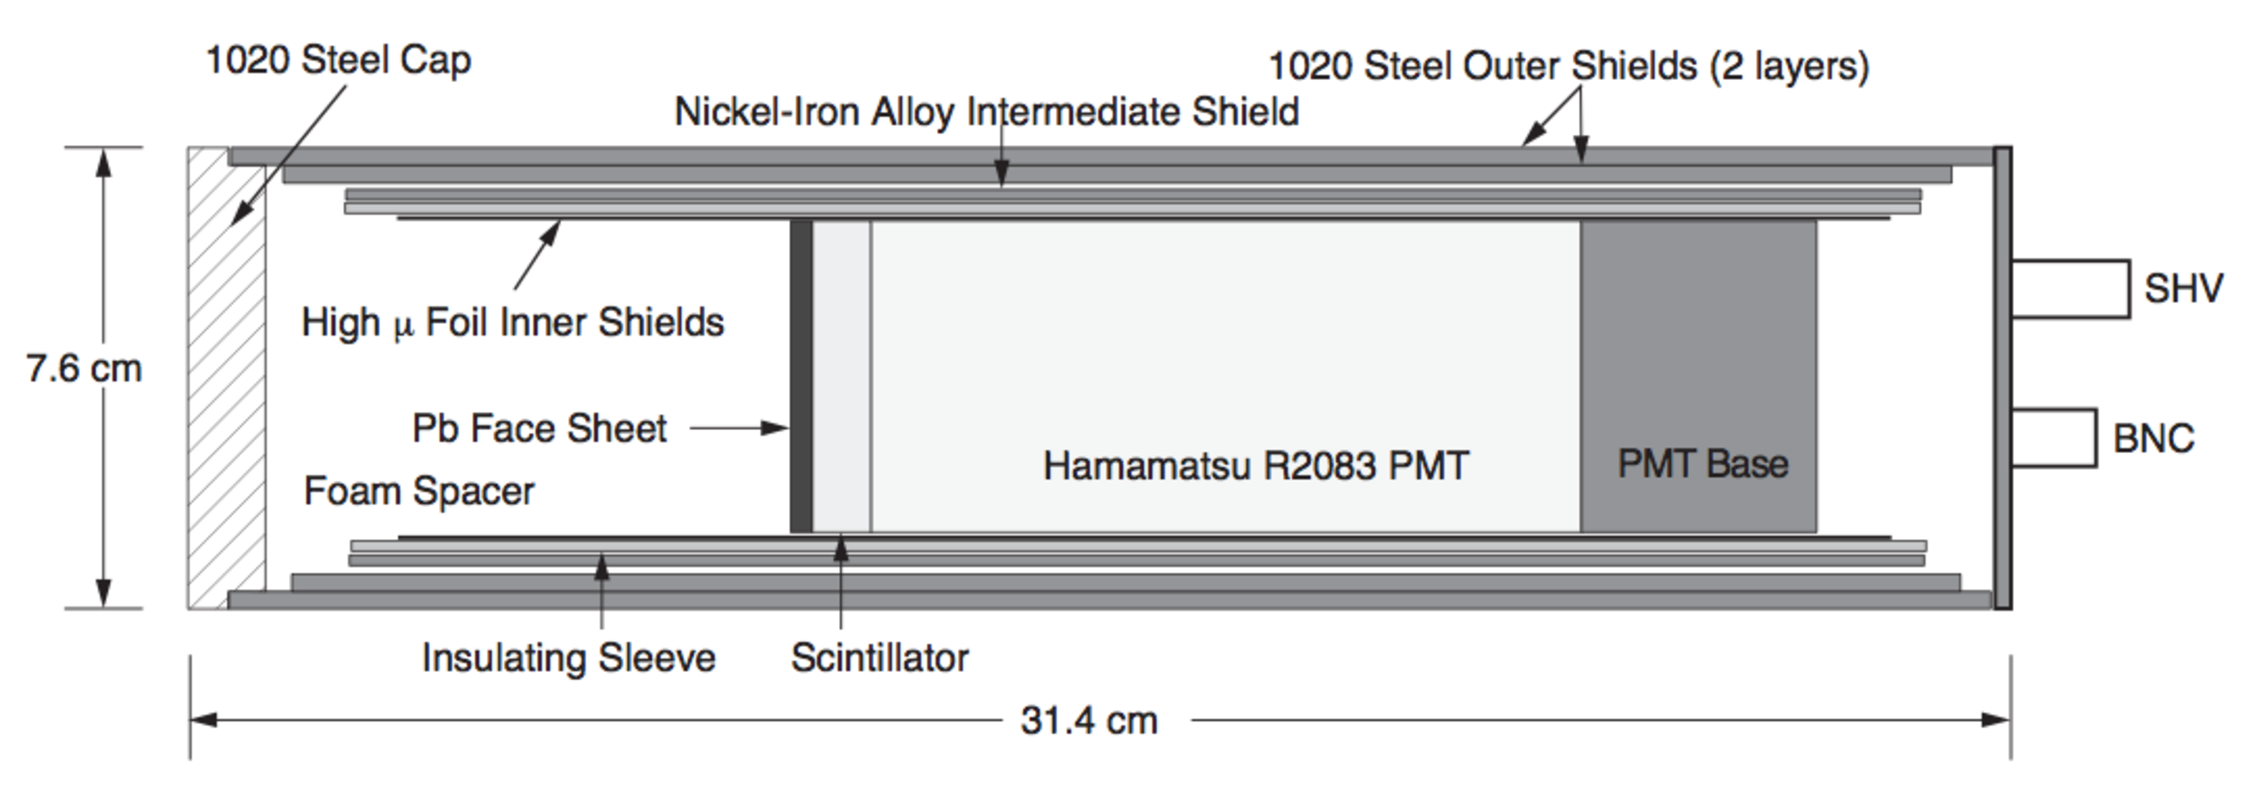
\includegraphics[width = .8\textwidth]{vpdDetector}
\caption[pVPD detector element]{A cross section of a pVPD detector element.}
\label{fig:vpdDetector}
\end{center}
\end{figure}

\begin{figure}
\begin{center}
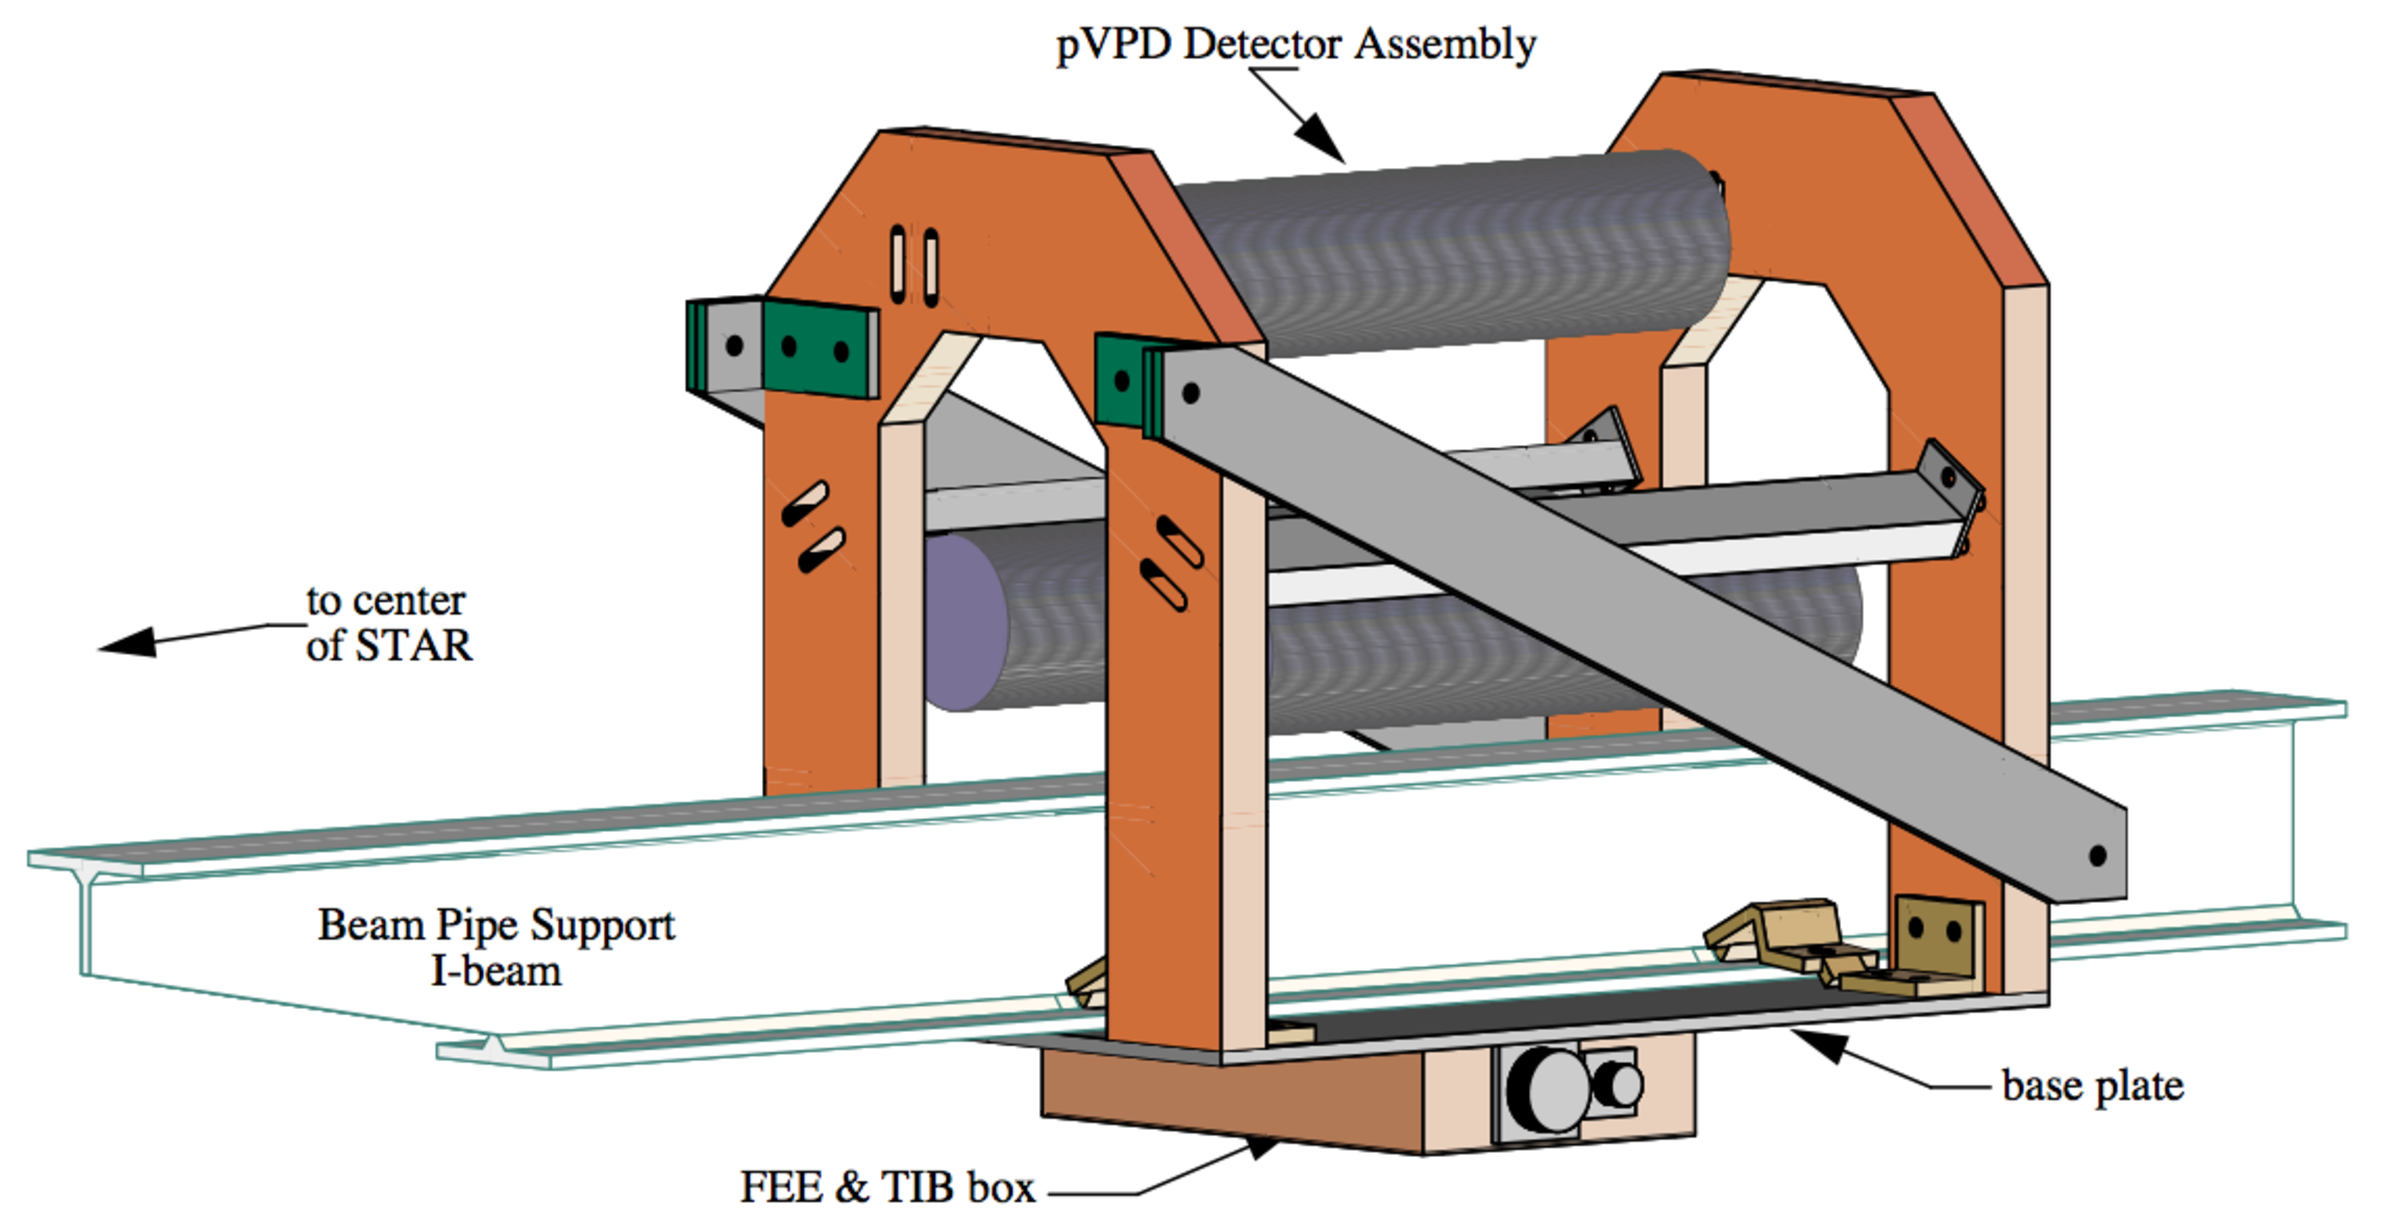
\includegraphics[width = .6\textwidth]{vpdAssembly}
\caption[pVPD Assembly]{The pVPD detector is mounted in the assembly.}
\label{fig:vpdAssembly}
\end{center}
\end{figure}

The pVPD starts the clock for the event and the TPCp stops it. The TPCp, shown in figure \ref{fig:starToF}, is again a scintillator/PMT detector. It covers about one unit in $\eta$ and about 1/60 of STAR's azimuthal coverage. It is encapsulated in an aluminum tray which is fastened to the outer field cage of the TPC at the 7 o'clock position. There are a total of 41 detector assemblies, each consisting of a 3.81 $\times$ 2 $\times$ 10 cm$^3$ BC420 plastic scintillator and a PMT. The PMTs are specially designed to work inside the STAR magnet.\cite{TOFppVPD}




\begin{figure}
\begin{center}
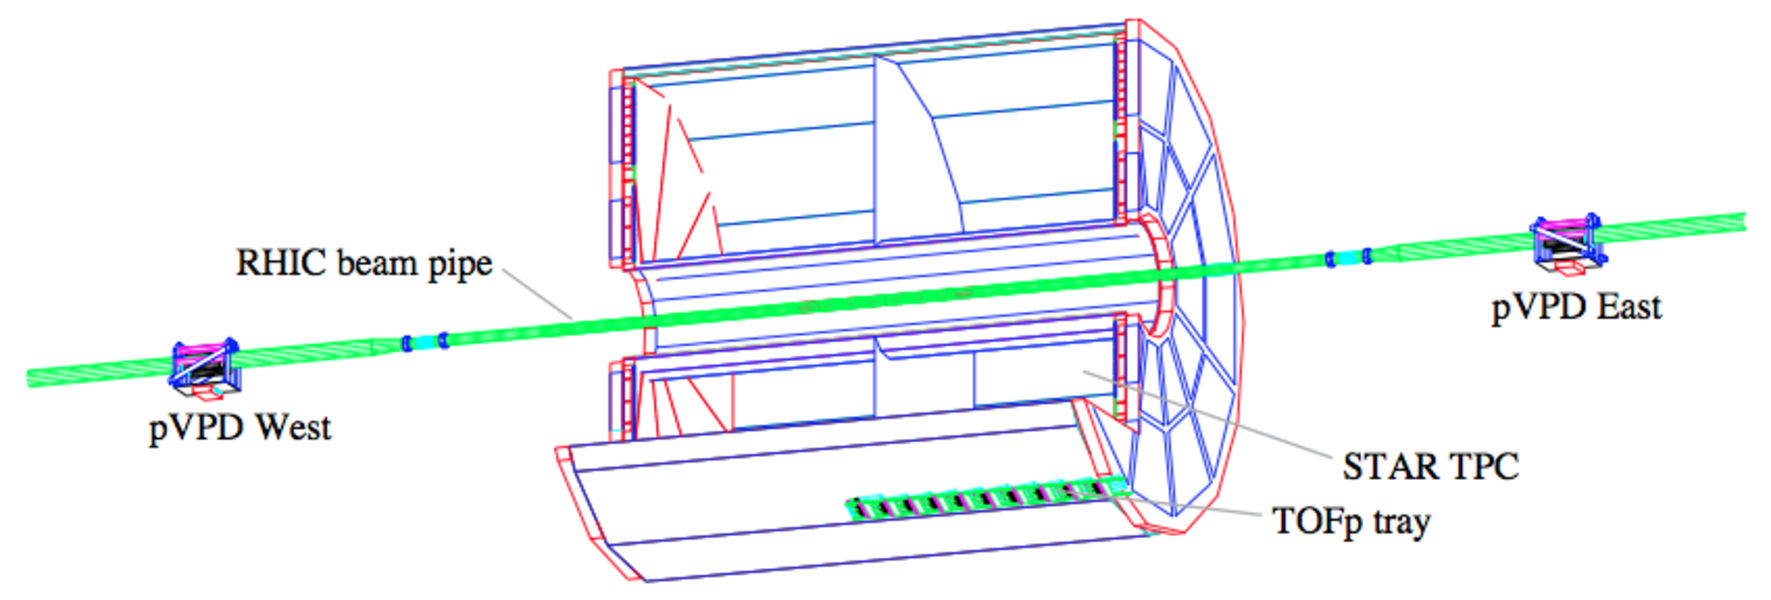
\includegraphics[width = .9\textwidth]{starToF}
\caption[STAR Time of Flight System]{The Time of Flight Patch is located near the botom of the STAR detector at the 7 o'colck positioin. Also shown here are the two pVPD detectors on either side of the STAR detector.}
\label{fig:starToF}
\end{center}
\end{figure}

Once the clock is stopped a value of $\beta$ for the track can be calculated as in equation \ref{eq:tof}. 

\begin{equation}
\label{eq:tof}
\frac{1}{\beta} = \frac{c\tau}{s}
\end{equation}
%
Here $c$ is the speed of light, $\tau$ is the time measured by the time of flight system, and $s$ is the path length of the track using the reconstructed path of the TPC. From here the mass of the particle can be found using the momentum of the track measured in the TPC.

\begin{equation}
\label{eq:mtof}
M^2 = \frac{p^2}{\beta^2} - 1
\end{equation}


\section{STAR triggers}

\section{Particle Identification}

\chapter{Theoretical background}

The differential cross section for the scattering process $P^\uparrow P \rightarrow \pip\pim + X$

The differential cross section for a transversely polarized quark, $b$, in a transversely polarized proton scattering off an unpolarized quark, $a$, in an unpolarized proton then fragmenting into a \pair pair is given in equation \ref{eq:crossSecUT_3}.\cite{bacchettaRedici2}


%\begin{equation}
%\label{eq:crossSecUT}
%d\sigma_{UT} \propto \ptpair |\overrightarrow{s_a}| \sin(\phirs) \int dx_a dx_b h_1(x_a) f_1(x_b) \frac{d\Delta\hat{\sigma}_{a^\uparrow b \rightarrow c^\uparrow d}}{d\hat{t}}H_1^{\sphericalangle c} \left(z,{\mpair}^2\right) 
%\end{equation}
%\begin{equation}
%\label{eq:crossSecUT_2}
%d\sigma_{UT} = 2\ptpair \sum_{a,b,c,d} |\overrightarrow{s_a}| \sin(\phirs)  \int \frac{dx_a dx_b}{8\pi^2 z_c} h_1(x_a) f_1(x_b) \frac{d\Delta\hat{\sigma}_{a^\uparrow b \rightarrow c^\uparrow d}}{d\hat{t}}\sin\theta H_1^{\sphericalangle c} \left(z_c,\cos\theta, {\mpair}^2\right) 
%\end{equation}

\begin{align}
\label{eq:crossSecUT_3}
d\sigma_{UT} = 2\ptpair \sum_{a,b,c,d} |\boldsymbol{s}_b| \frac{|\boldsymbol{R}|}{\mpair}\sin(\phirs) & \int \frac{dx_a dx_b}{8\pi^2 z_c} f_1(x_a) h_1(x_b) \frac{d\Delta\hat{\sigma}_{a b^\uparrow \rightarrow c^\uparrow d}}{d\hat{t}} \nonumber \\ 
&\times \sin\theta H_1^{\sphericalangle c} \left(\bar{z}_c,\cos\theta, {\mpair}^2\right) 
\end{align}
%\begin{align}
%\label{eq:crossSecUT_3}
%d\sigma_{UT} = 2\ptpair \sum_{a,b,c,d} |\overrightarrow{s_a}| \sin(\phirs) & \int \frac{dx_a dx_b}{8\pi^2 z_c} h_1(x_a) f_1(x_b) \frac{d\Delta\hat{\sigma}_{a^\uparrow b \rightarrow c^\uparrow d}}{d\hat{t}} \nonumber \\ 
%&\times \sin\theta H_1^{\sphericalangle c} \left(z_c,\cos\theta, {\mpair}^2\right) 
%\end{align}
%
Here $|\bm{s}_b|$ is the spin direction of the polarized proton. In our exeriment we always want the polarized proton's spin to be either up or down. However we can't always the it 100\% polarized so we use the polarization of the fill as $|\bm{s}_b|$. Moving on, $\phirs$ is the relative orientation of the outgoing pion pair shown in figure \ref{fig:angleDeff}, $z_c$ is the fraction of the fragmenting quark momentum the pion pair retains, and $\theta$ is the azimuthal angle of the outgoing \pair piar. The difference in momenta of the final state \pair pair is $\boldsymbol{R}$. The hard scattering cross section of a transversely polarized quark $b$ scattering off of an unpolarized quark $a$ into a transversely polarized quark $c$ and an unpolarized quark $d$ $\frac{d\Delta\hat{\sigma}_{a b^\uparrow \rightarrow c^\uparrow d}}{d\hat{t}}$ can be found in Ref \cite{bacchettaRedici2}.
We can make better sense of the above equation by looking closely at each part. First we see the magnitude of the \pair pair transverse momentum. We then see the polarization of the beam. Next is the sinusoidal modulation of the production of \pair pairs. Inside the integral we have the unpolarized distribution function $f_1$ due to the unpolarized  quark $a$ and the transversity distribution function $h_1$ due to the polarized quark $b$. After this we see the elementary scattering cross section of unpolarized quark $a$ scattering off transversely polarized quark $b$ into a transversely polarized quark $c$ and an unpolarized quark $d$. Quark $c$ goes on to fragment into $\pip\pim + X$ described by the IFF $H_1^{\sphericalangle}$ while $d$ goes undetected. 

Comparing this to the cross section when both initial state quarks are unpolarized we see several similarities.
\begin{equation}
\label{eq:crossSecUU}
d\sigma_{UU} = 2 \ptpair \sum_{a,b,c,d} \int \frac{dx_adx_b}{8\pi^2z_c} f_1^a(x_a)f_1^b(x_b) \frac{d\hat{\sigma}_{ab \rightarrow cd}}{d\hat{t}}D_1^c(\bar{z_c},\textnormal{cos}\theta_C,M_C^2)
\end{equation}

As similar as equations \ref{eq:crossSecUT_3} and \ref{eq:crossSecUU} looks there are some important differences worth noting. Obviously the polarization isn't there since we now are dealing with unpolarized scattering. The sinusoidal modulation has also disappeared. The transversity distribution has turned into a second unpolarized distribution, and the IFF has turned into $D_1^c$ which is the unpolarized counterpart to the IFF.   

The most important thing to mention is that the sine modulation seen in unpolarized-polarized (U-T) scattering is not seen in unpolarized-unpolarized (U-U) scattering. This means that there is a bias to the yield of \pair pairs in U-T scattering when compared to U-U scattering. We can observe this by looking at the number of \pair pairs at a given value of $\phirs$ when the polarization of the proton beam is $\hat{y}$ vs the number when the polarization is $-\hat{y}$. We then normalize by the number we see at that value of $\phirs$ for U-U scattering. 

\begin{equation}
\label{eq:asymCS}
A_{UT} \sin (\phirs) =\frac{1}{|\bm{s}_b|} \frac{d\sigma^\uparrow - d\sigma^\downarrow}{d\sigma_{UU}}
\end{equation}

In our experiment we never scatter unpolarized protons, so we have to be cleaver about the cross section seen in the denominator of equation \ref{eq:asymCS}. If we sum over the two spin states we are left with the entire unpolarized cross section $d\sigma^\uparrow + d\sigma^\downarrow = d\sigma_{UU}$. [cite thesis and papers by Baccheta also maybe add the jeffe paper and info] 

This is the only source of a single spin asymmetry at leading twist.\cite{bacchettaRedici2}

\begin{equation}
\label{eq:asymCS}
A_{UT} \sin (\phirs) =\frac{1}{|\bm{s}_b|} \frac{d\sigma^\uparrow - d\sigma^\downarrow}{d\sigma^\uparrow + d\sigma^\downarrow}
\end{equation}

Important physics can be seen by preforming a partial wave expansion of the cross section. Namely $\sin \theta H_1^\sphericalangle$ can be expanded. Looking at the first two terms in the expansion, 

%\begin{equation}
%\label{eq:partialwaveexpansion}
%\sin \theta H_1^{\sphericalangle c} (\bar{z_c},\cos \theta, {\mpair}^2) \approx H^{\sphericalangle c}_{1,ot}(\bar{z_c},{\mpair}^2) \sin\theta + H^{\sphericalangle c}_{1,lt}(\bar{z_c},{\mpair}^2) \sin\theta \cos\theta
%\end{equation}

\begin{align}
\label{eq:partialwaveexpansion}
\sin \theta H_1^{\sphericalangle c} (\bar{z_c},\cos \theta, {\mpair}^2) \approx &H^{\sphericalangle c}_{1,ot}(\bar{z_c},{\mpair}^2) \sin\theta \nonumber \\
+ &H^{\sphericalangle c}_{1,lt}(\bar{z_c},{\mpair}^2) \sin\theta \cos\theta
\end{align}
%
The first term, S/P wave interference, is due to the interference between amplitudes for a decay into an $L = 0$  \pair pair and an $L = 1$ transversely polarized \pair pair. The second term, P/P wave interference, is due to the interference between amplitudes for a decay into an $L = 1$ \pair pair and an $L = 1$ transversely polarized \pair pair. The $L=1$ contributions come from a \pair pair that went through a spin-1 intermediate state. One such intermediary we have the ability and statistics to look for is the $\rho$ meson. We expect there to be an enhancement in the IFF, and thus the asymmetry, in the invariant mass region of the $\rho$ (770 MeV). \cite{bacchettaRedici2, Tang}    



\begin{figure}
\begin{center}
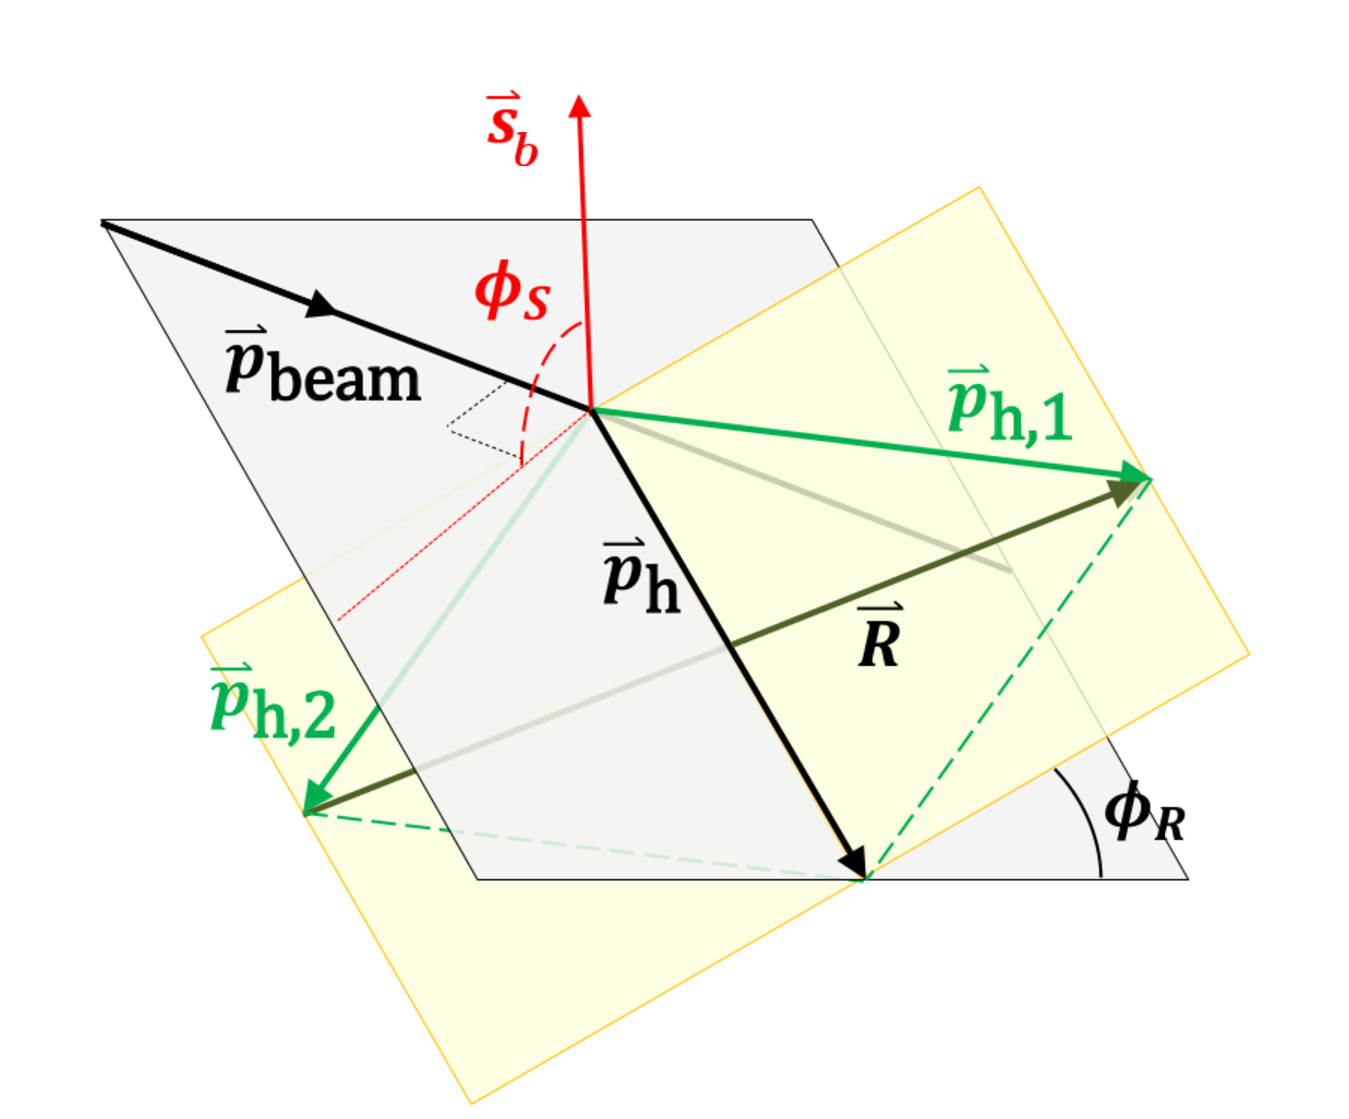
\includegraphics[width = 1\textwidth]{IFF_frame_edit2}
\caption[Angles $\phis$ and $\phir$]{Visual representation of angles $\phi_R$ and $\phi_S$ \\ $\vec{p}_{h,1}$ is the momentum of the positive hadron while  $\vec{p}_{h,2}$ is the momentum of the negative hadron.}
\label{fig:angleDeff}
\end{center}
\end{figure}




\chapter{2006 analysis and sim}
\label{chap:2006}

The 2006 data set gave us the first glimpse of this asymmetry. The analysis of the 2006 data set was done by Anselm Vossen. The 2006 run had only a small integrated luminosity of 200 GeV transverse proton proton collisions. Due to this, the data set was small and you couldn't look at everything you wanted to. 


Figure \ref{fig:ansM} shows the asymmetry as a function of the pion pair invariant mass. As hinted from the theory there is an increase in the asymmetry around the $\rho$ meson mass for both forward and backward pairs. 


 \begin{figure}
\begin{center}
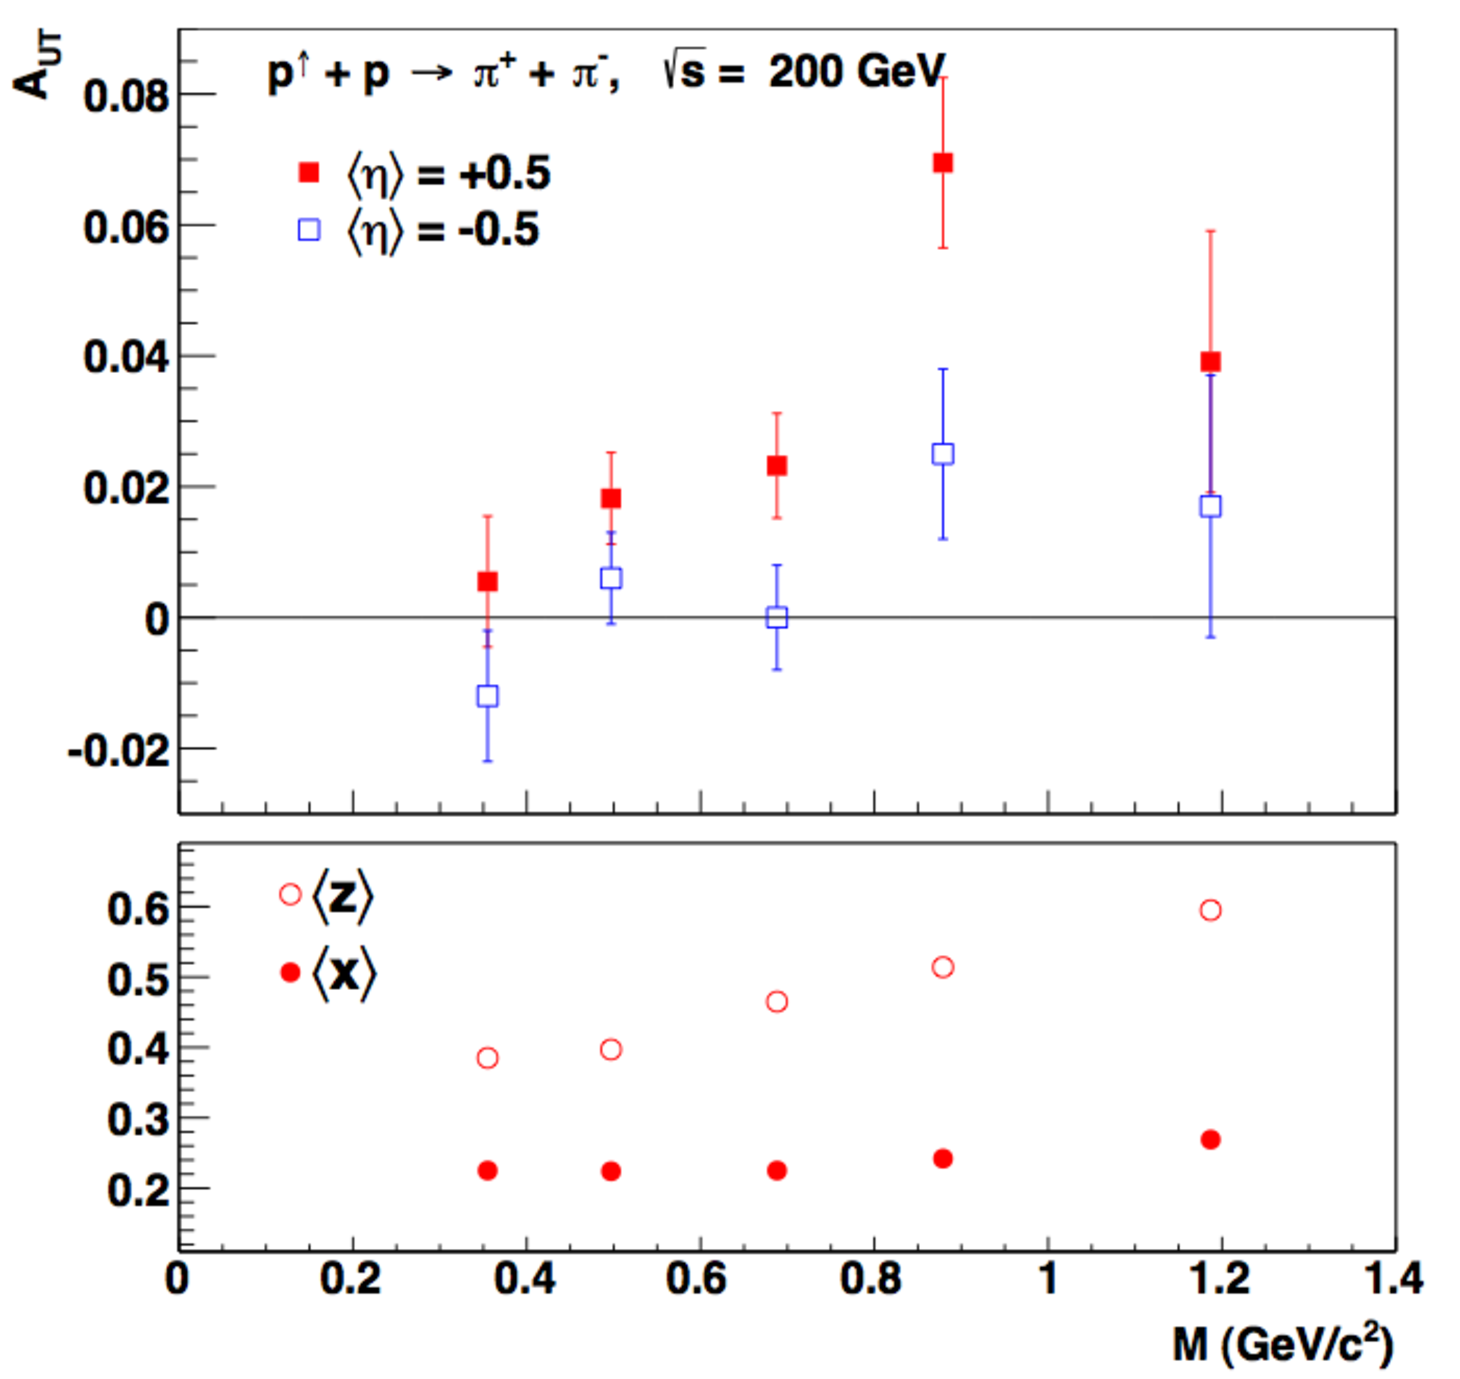
\includegraphics[width = 1\textwidth]{ansM_new}
\caption[$A_{UT}$ vs Invariant Mass in 2006 data set]{Asymmetry versus invariant mass of the \pair pair for the 2006 data set for pairs scattering in the forward direction (red) and in the backward direction (blue).}
\label{fig:ansM}
\end{center}
\end{figure}


Varying the opening angle of the pion pair grants access to the z dependence of the asymmetry. The fraction of the fragmenting quark momentum the pion pair retains, z, influences the size of the IFF. It turns out the asymmetry increases as the opening angle decreases as seen in figure \ref{fig:ansAng}.

 \begin{figure}
\begin{center}
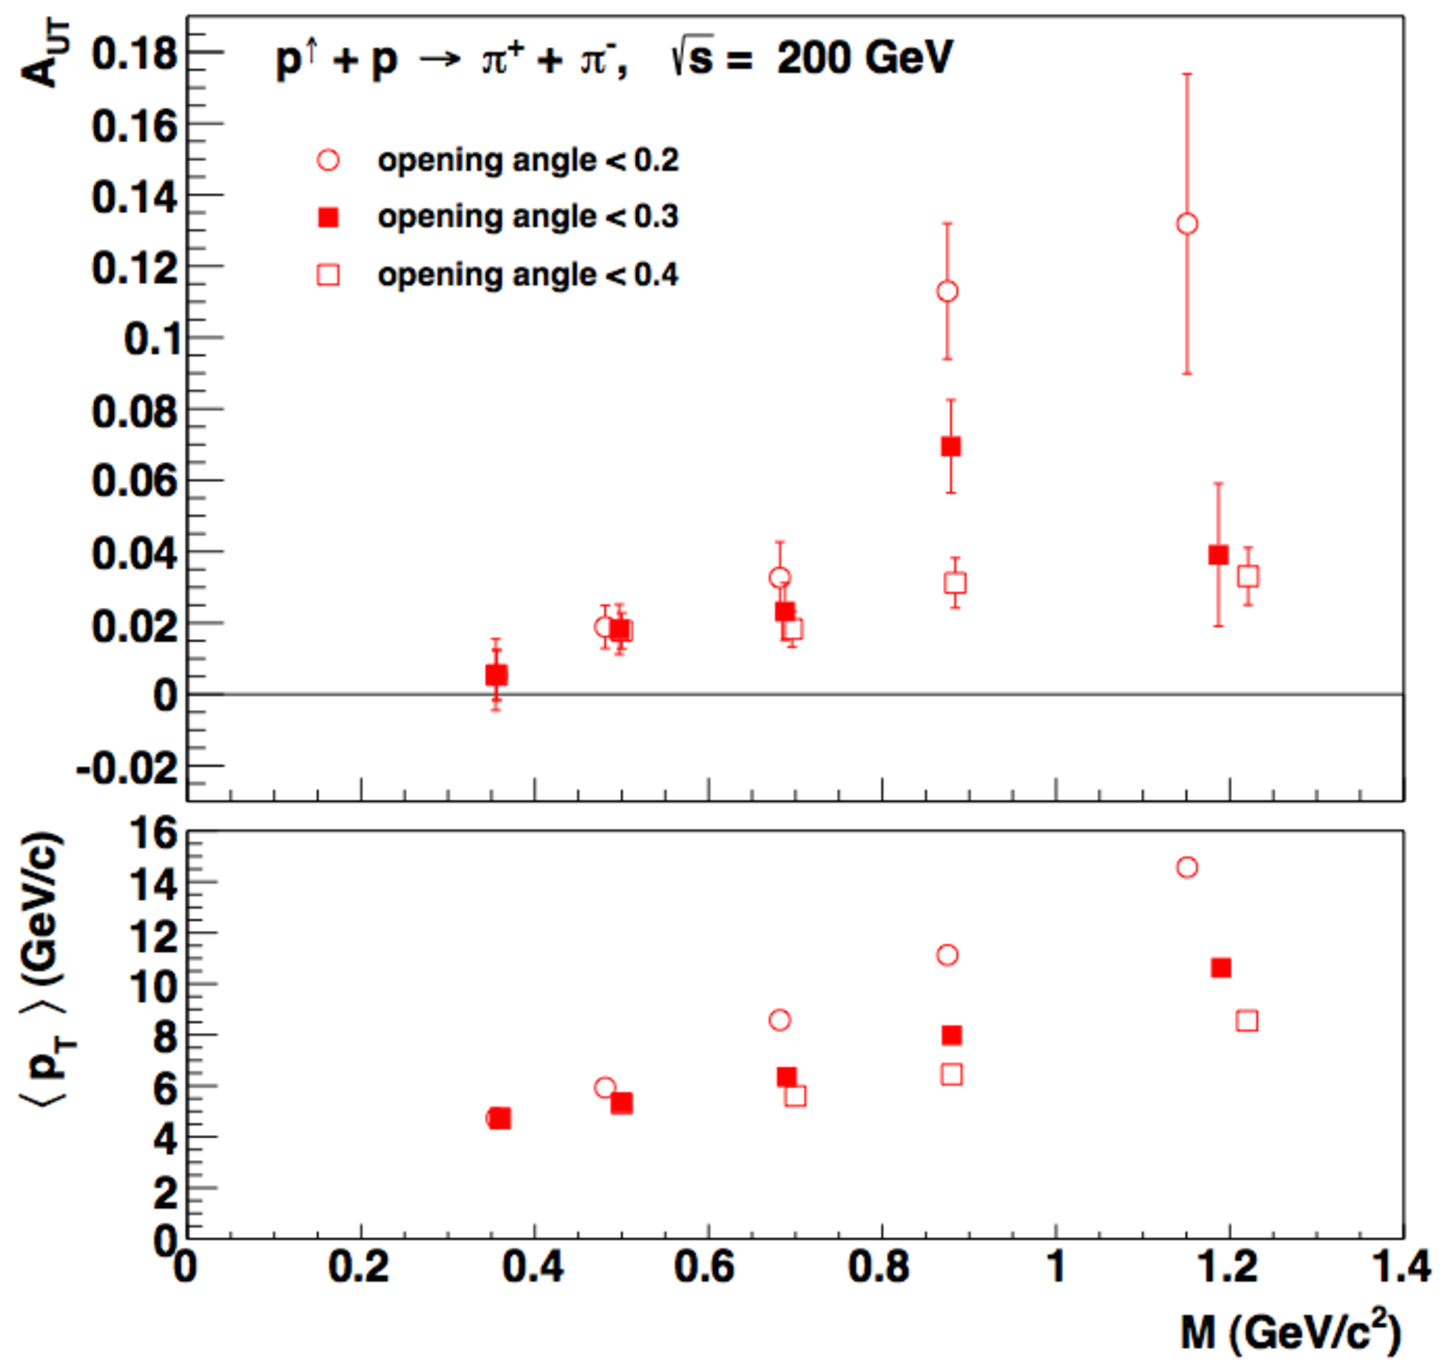
\includegraphics[width = 1\textwidth]{ansAngles_new}
\caption[$A_{UT}$ for different opening angles]{Asymmetry versus invariant mass of the \pair pair for the 2006 data set for different opening angles of pairs are scattered into the forward direction.}
\label{fig:ansAng}
\end{center}
\end{figure}

As stated previously, $\etapair$ acts as a stand in for the momentum fraction of the polarized parton, as a larger partonic momentum fraction will cause the pion pair to be produced in a more forward direction. The asymmetry is plotted as a funtion of $\etapair$ in figure \ref{fig:ansEta}. As one might expect, the asymmetry is larger the more forward the pion pair is. This is explained by the fact that more forward pairs result from polarized partons with larger momentum fractions allowing for a larger spin transfer. 


 \begin{figure}
\begin{center}
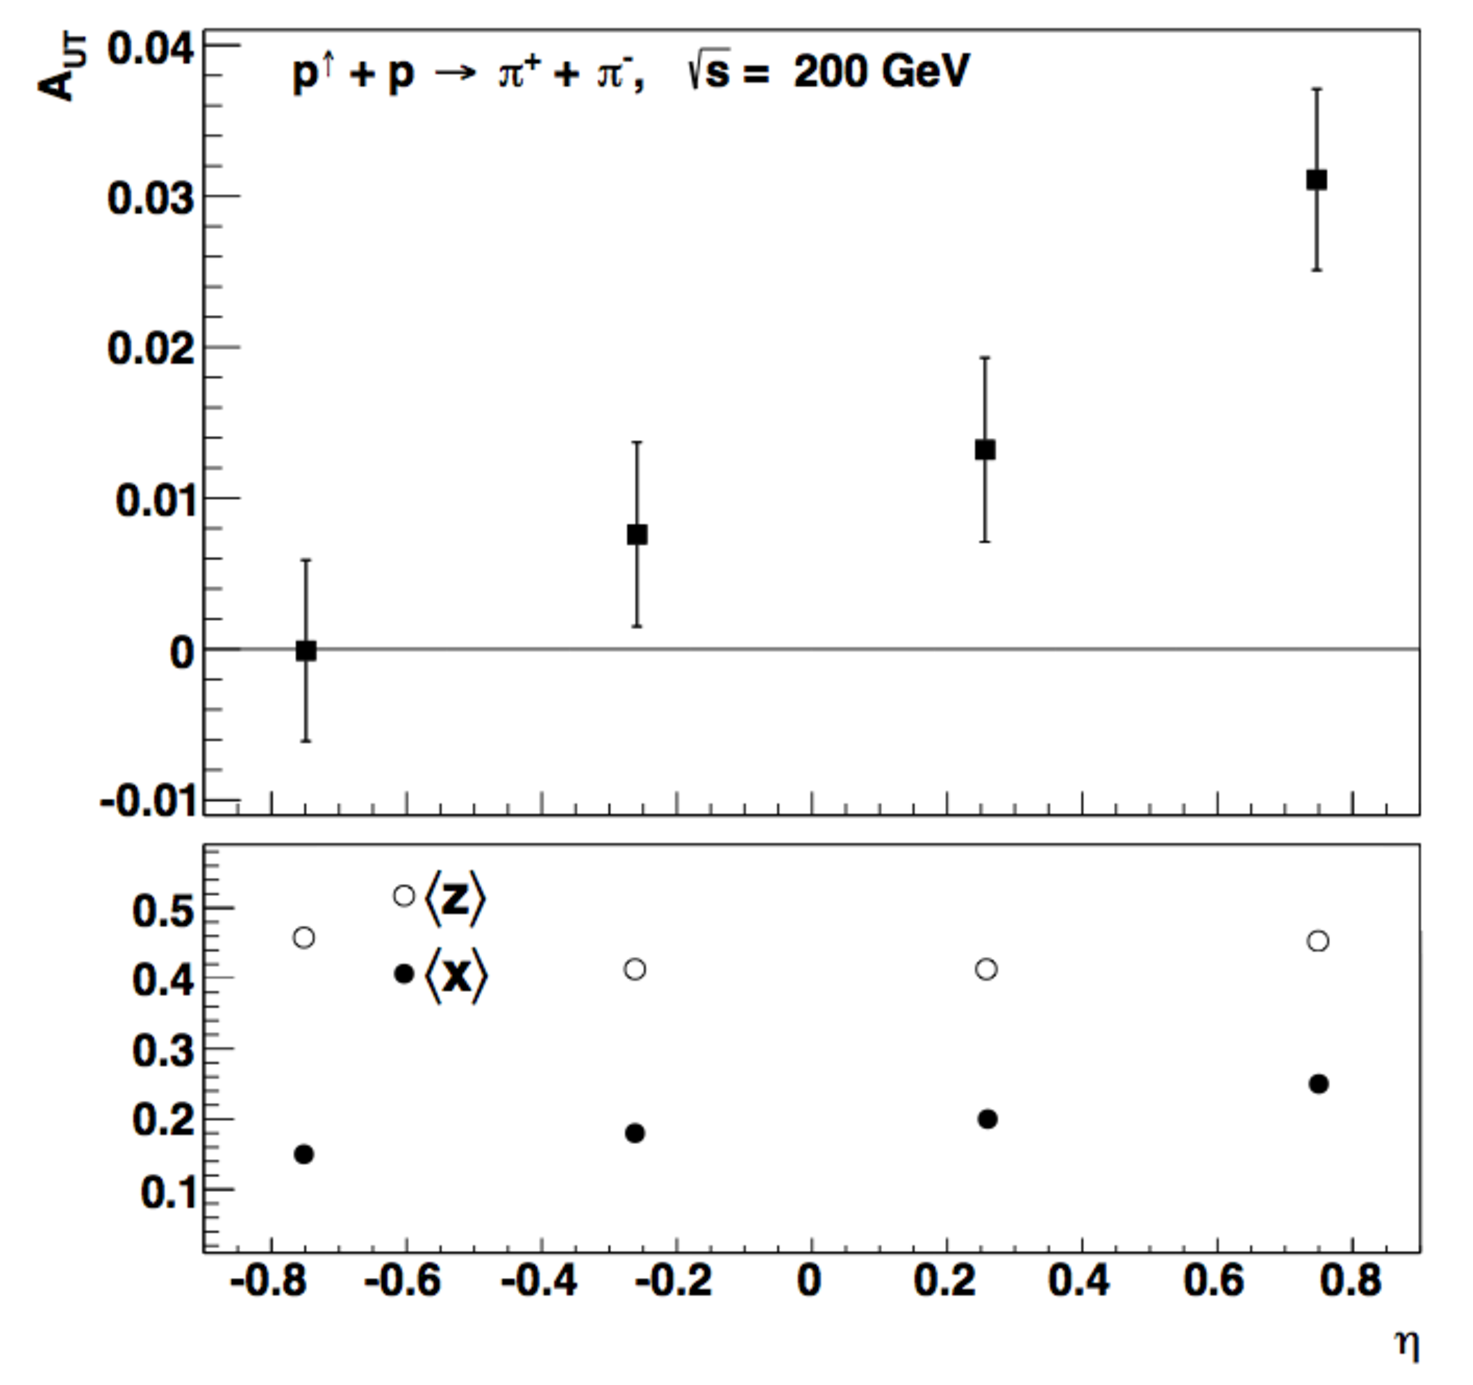
\includegraphics[width = 1\textwidth]{ansEta_new}
\caption[$A_{UT}$ vs $\etapair$ in 2006 data set]{Asymmetry versus $\etapair$ for the 2006 data set}
\label{fig:ansEta}
\end{center}
\end{figure}


 \begin{figure}
\begin{center}
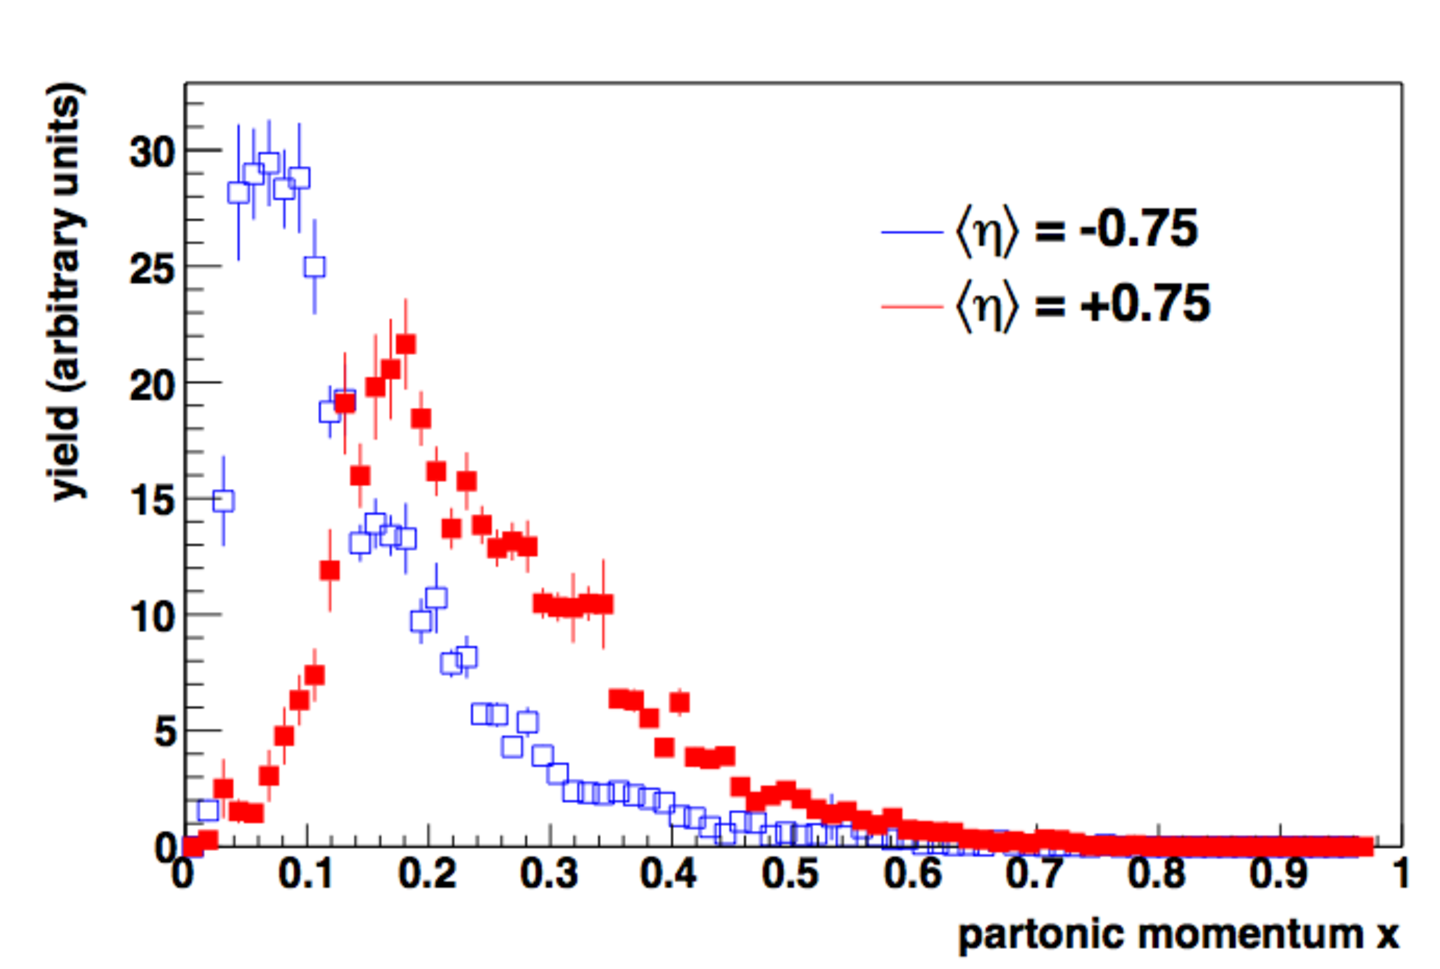
\includegraphics[width = 1\textwidth]{2006SimX}
\caption[Partonic momentum fraction in 2006 simulation forward and backward \pair pair]{Partonic momentum fraction $x$ for the parton from the polarized proton in the forward (red) and backward (blue) direction}
\label{fig:2006SimX}
\end{center}
\end{figure}


These results are the first sign of nonzero asymmetries in \pair pair correlation in polarized proton collisions. More can be read about the 2006 study in reference \cite{} ADD CITATION.



\chapter{2012 IFF}

\section{Data Set and Cuts?}

\section{Particle Identification and Contamination}



As charged particles traverse the TPC, they deposit energy in the TPC gas. This energy loss is different for different particles. A value, $n_\sigma(\pi)$, is given to each track in an event describing how many standard deviations away it is from an ideal pion on the ionization energy loss curve shown in figure \ref{fig:tpcDedx2}; the ideal curves shown as black lines. Each track is also given values of $n_\sigma(p)$, $n_\sigma(k)$, and $n_\sigma(e)$ describing how close they are to ideal protons, kaons, and electrons. For example if a track has an $n_\sigma(\pi)$ value of zero, it is very likely a pion and should be included in the analysis. 

 \begin{figure}
\begin{center}
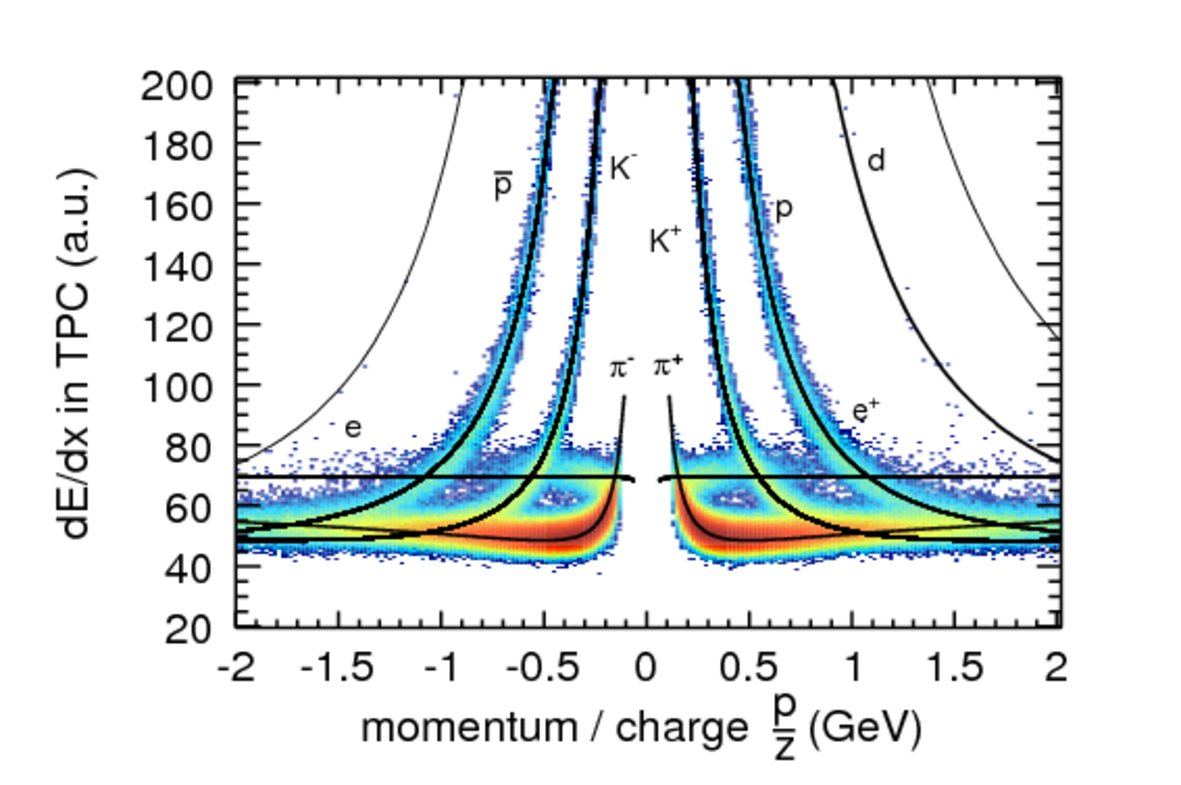
\includegraphics[width = .8\textwidth]{TPC_dedx2}
\caption[Ionization energy loss in TPC]{Ionization energy loss as a function of particle momentum divided by electric charge for TPC tracks}
\label{fig:tpcDedx2}
\end{center}
\end{figure}


If the data set strictly contained pions, the $n_\sigma(\pi)$ distribution would be gaussian centered around 0. However as seen in figure \ref{fig:nSigExample} it is not exactly gaussian. Although it looks gaussian near $n_\sigma(\pi) = 0$, there is a clear shoulder on the left side due to kaon and proton contamination and a much less observable shoulder to the right from electron contamination. To account for this contamination we fit the $n_\sigma(\pi)$ distribution with a 5-gaussian fit; one gaussian for each particle species plus one gaussian to account for the tail at high $n_\sigma(\pi)$ most likely due to pile up or merged tracks. 

Several of the degrees of freedom of the fit can be constrained for physical reasons. First the expected $n_\sigma(\pi)$ value of an ideal kaon can be readily found from fitting a plot of $n_\sigma(\pi)$ vs $n_\sigma(k)$ as in figure \ref{fig:nSignSig}. The separation between the pion gaussian and the kaon gaussian in the 5-gaussian fit is required to be equal to the value of $n_\sigma(\pi)$ at $n_\sigma(k) = 0$. This is repeated to constrain the separation between the pion gaussian and the proton gaussian as well as the separation between the pion and electron gaussains. Secondly since kaons and protons are required to have the same width. Third the "pile up" gaussian is required to have a smaller amplitude than and be located at a larger $n_\sigma(\pi)$ than the electron gaussian. This is to make sure it actually does fit the high $n_\sigma(\pi)$ tail. This tail is more prominent at higher track momentum but is sometimes absent at lower momentum.  

Armed with this fitting procedure, the location and amount of each particle species becomes clear (figure \ref{fig:nSigExampleFit}). A clean sample of pions can be found by selecting tracks with an $n_\sigma(\pi)$ between -1 and 2.5. This choice maximizes the number of pions included in the analysis while not compromising the purity of the pion sample too much.  


         
 \begin{figure}
\begin{center}
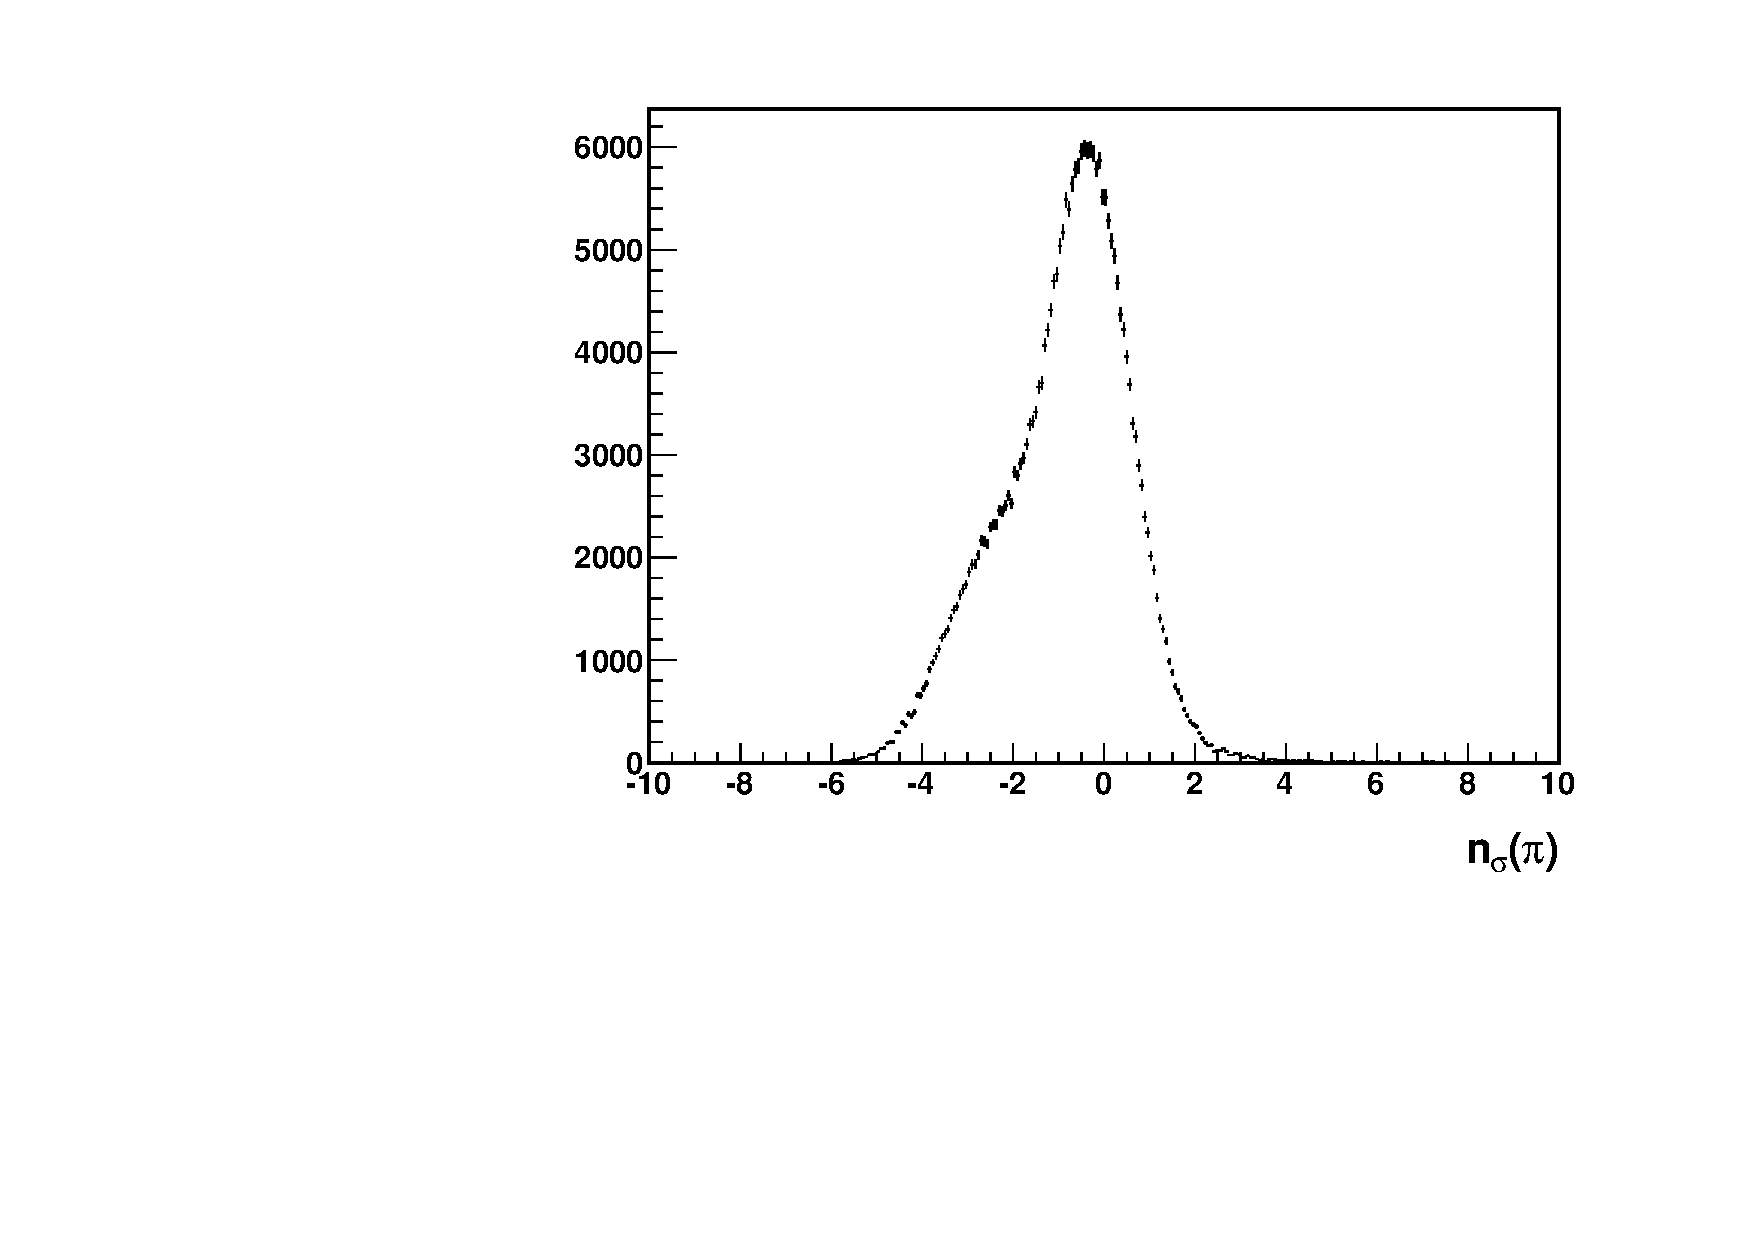
\includegraphics[width = .7\textwidth]{histogramExample.pdf}
\caption[$n_\sigma(\pi)$ distribution]{$n_\sigma(\pi)$ distribution of TCP tracks}
\label{fig:nSigExample}
\end{center}
\end{figure}



 \begin{figure}
\begin{center}
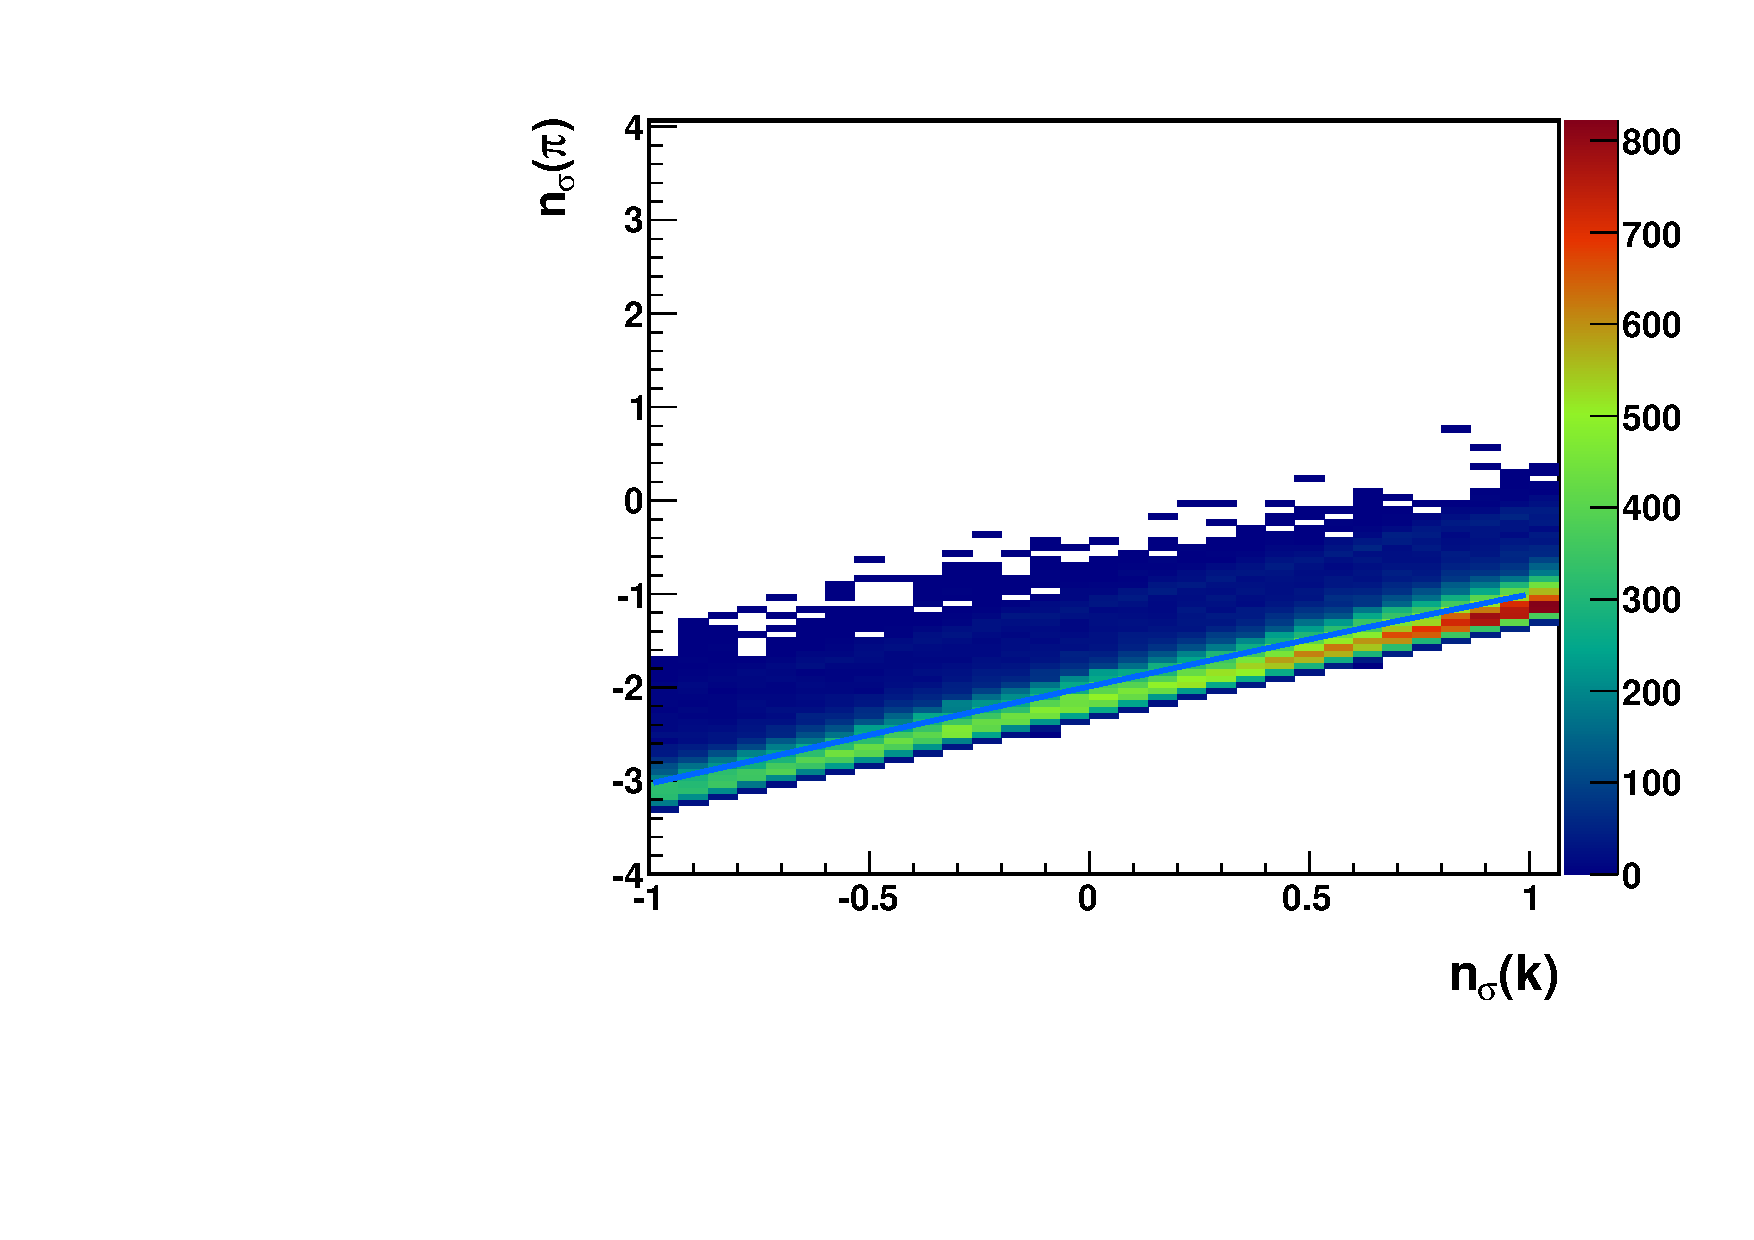
\includegraphics[width = .7\textwidth]{exampleNsigNsig.pdf}
\caption[$n_\sigma(\pi)$ versus $n_\sigma(k)$]{$n_\sigma(\pi)$ versus $n_\sigma(k)$ The blue line is a 3rd order polynomial fit of the profile. The $n_\sigma(\pi)$ value at $n_\sigma(k) = 0$ is taken as the separation between the pion gaussian and the kaon gaussian in the 5-gaussian fit.}
\label{fig:nSignSig}
\end{center}
\end{figure}



 \begin{figure}
\begin{center}
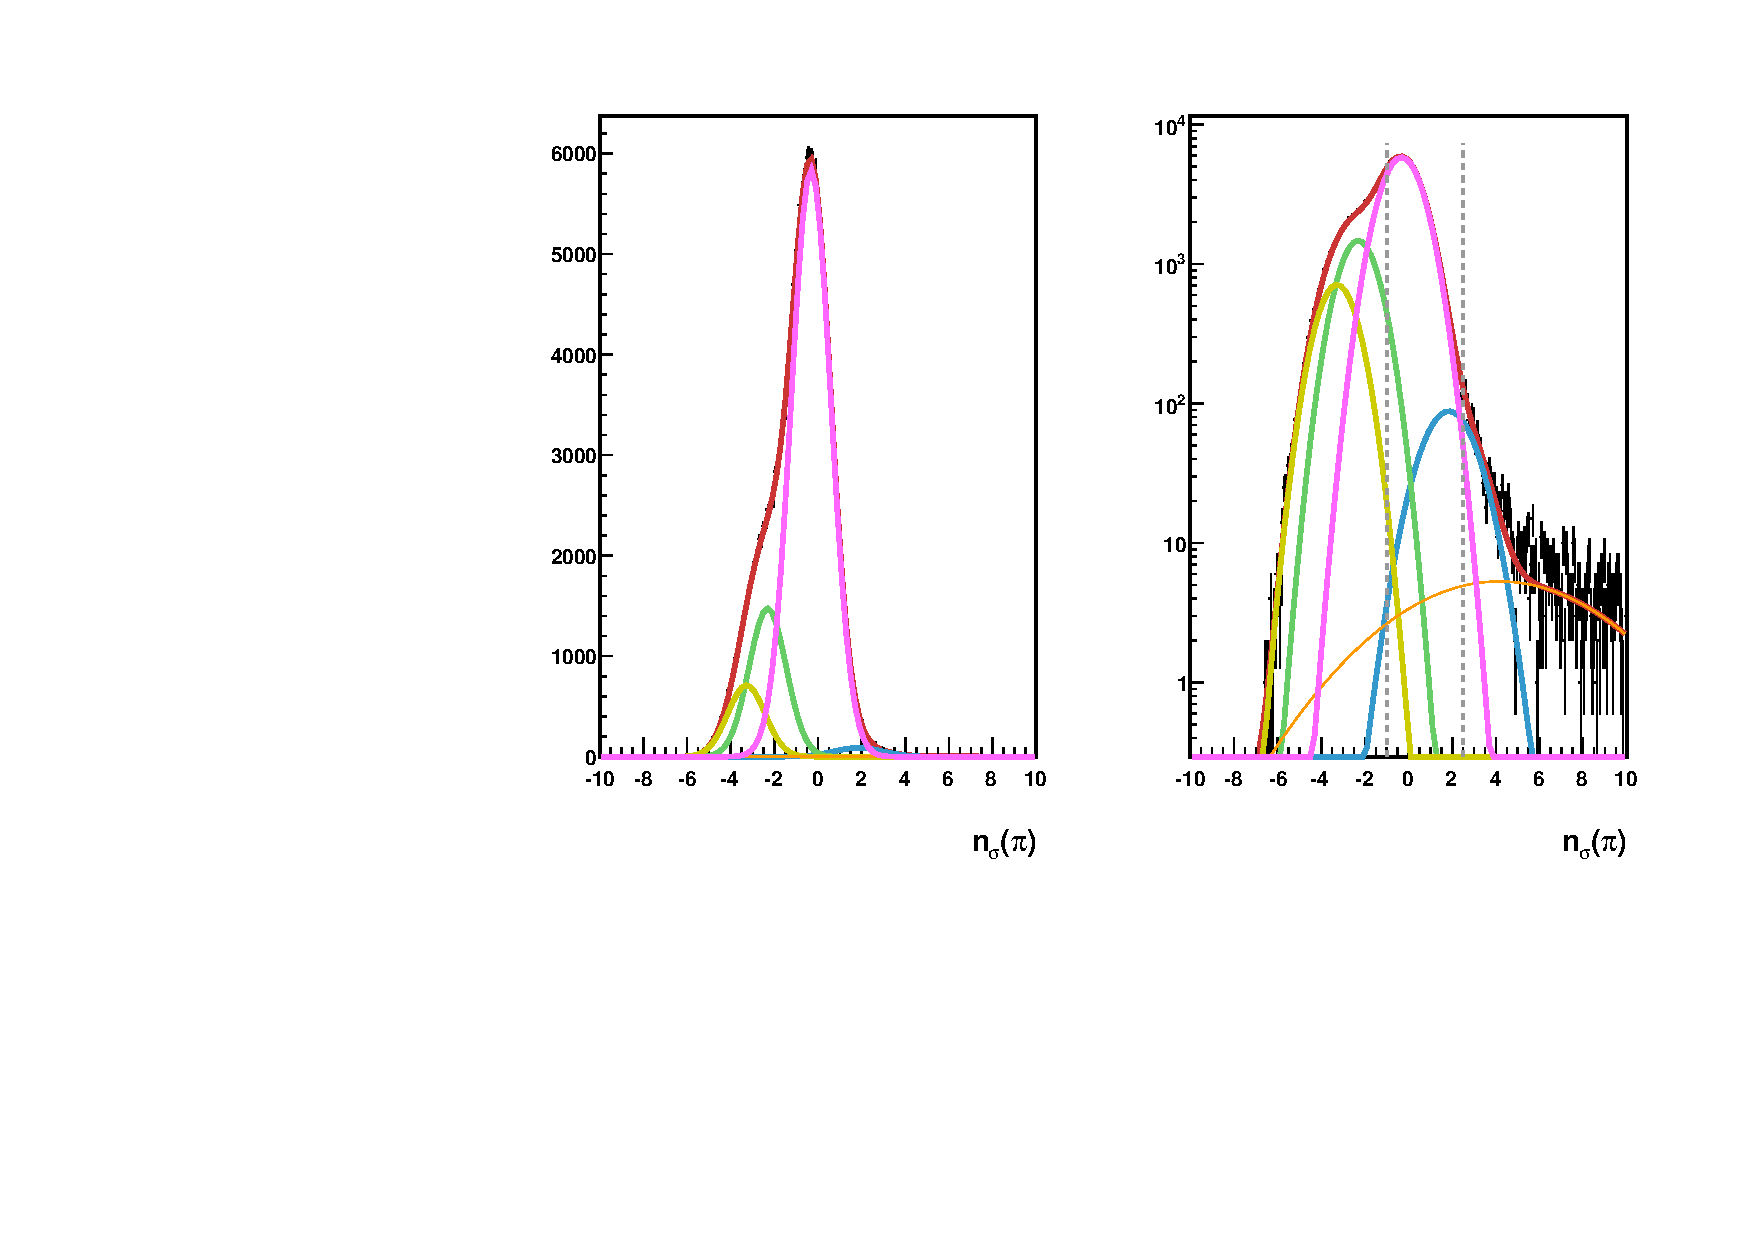
\includegraphics[width = 1\textwidth]{histogramExample2Fit.pdf}
\caption[5-gaussian fit of $n_\sigma(\pi)$ distribution]{5-gaussian fit of $n_\sigma(\pi)$ distribution. The pion peak is shown in pink, the kaon peak in green, the proton peak in yellow, the electron peak in blue, and the pile up peak in orange. Right panel is a log scale for better visibility of smaller peaks. The dashed lines indicate the $-1 < n_\sigma(\pi) < 2.5$ range chosen for the analysis.}
\label{fig:nSigExampleFit}
\end{center}
\end{figure}


When interpreting the asymmetry results, it is important to quantify the pion purity of the data. As the ionization energy loss curves show (figure \ref{fig:tpcDedx2}), the energy loss depends on track momentum. More importantly, each particle species behaves differently and even cross around track momentum between 1 and 2 GeV making it hard to determine the contamination of the pion data set all at once. Instead the data set is broken into 5 bins in track momentum and 5 in detector $\theta$ (the polar angle measured with respect to the beam direction). In each of these bins, the 5-gaussian fitting procedure is repeated. The 5 gaussian fits are shown in figures \ref{fig:5gaus4} to \ref{fig:5gaus0}. For highest 4 track momentum bins, the pion fraction is calculated by integrating the pion gaussian from $n_\sigma(\pi) = -1$ to $n_\sigma(\pi) = 2.5$ and dividing by the integral of the total fit in the same range. In the smallest track momentum bin, the ionization energy loss curves of protons and pions start to overlap, prohibiting an accurate determination of the pion fraction using the same method. Luckily in this low momentum range, the time of flight can accurately distinguish proton and pions very easily. Using the ToF, the particle mass may be computed. A two dimensional histogram of $M^2$ and $n_\sigma(\pi)$ shown in figure \ref{fig:tofPlot} shows how the protons are distinguished from pions. Any particle above the red line is taken to be a proton. The proton fraction is then computed by dividing the number of tracks above the red line by the total number of tracks. The kaon, electron, and pile up fractions are computed from integrating the 5-gaussian fits, and the pion fraction is determined by the relationship: $1-F_k - F_p - F_e - F_{pile-up} = F_\pi$. Pion fractions for the kinematic bins used in the asymmetry analysis were computed from the pion fractions known in track momentum and detector $\theta$ using a weighted mean. 






 \begin{figure}
\begin{center}
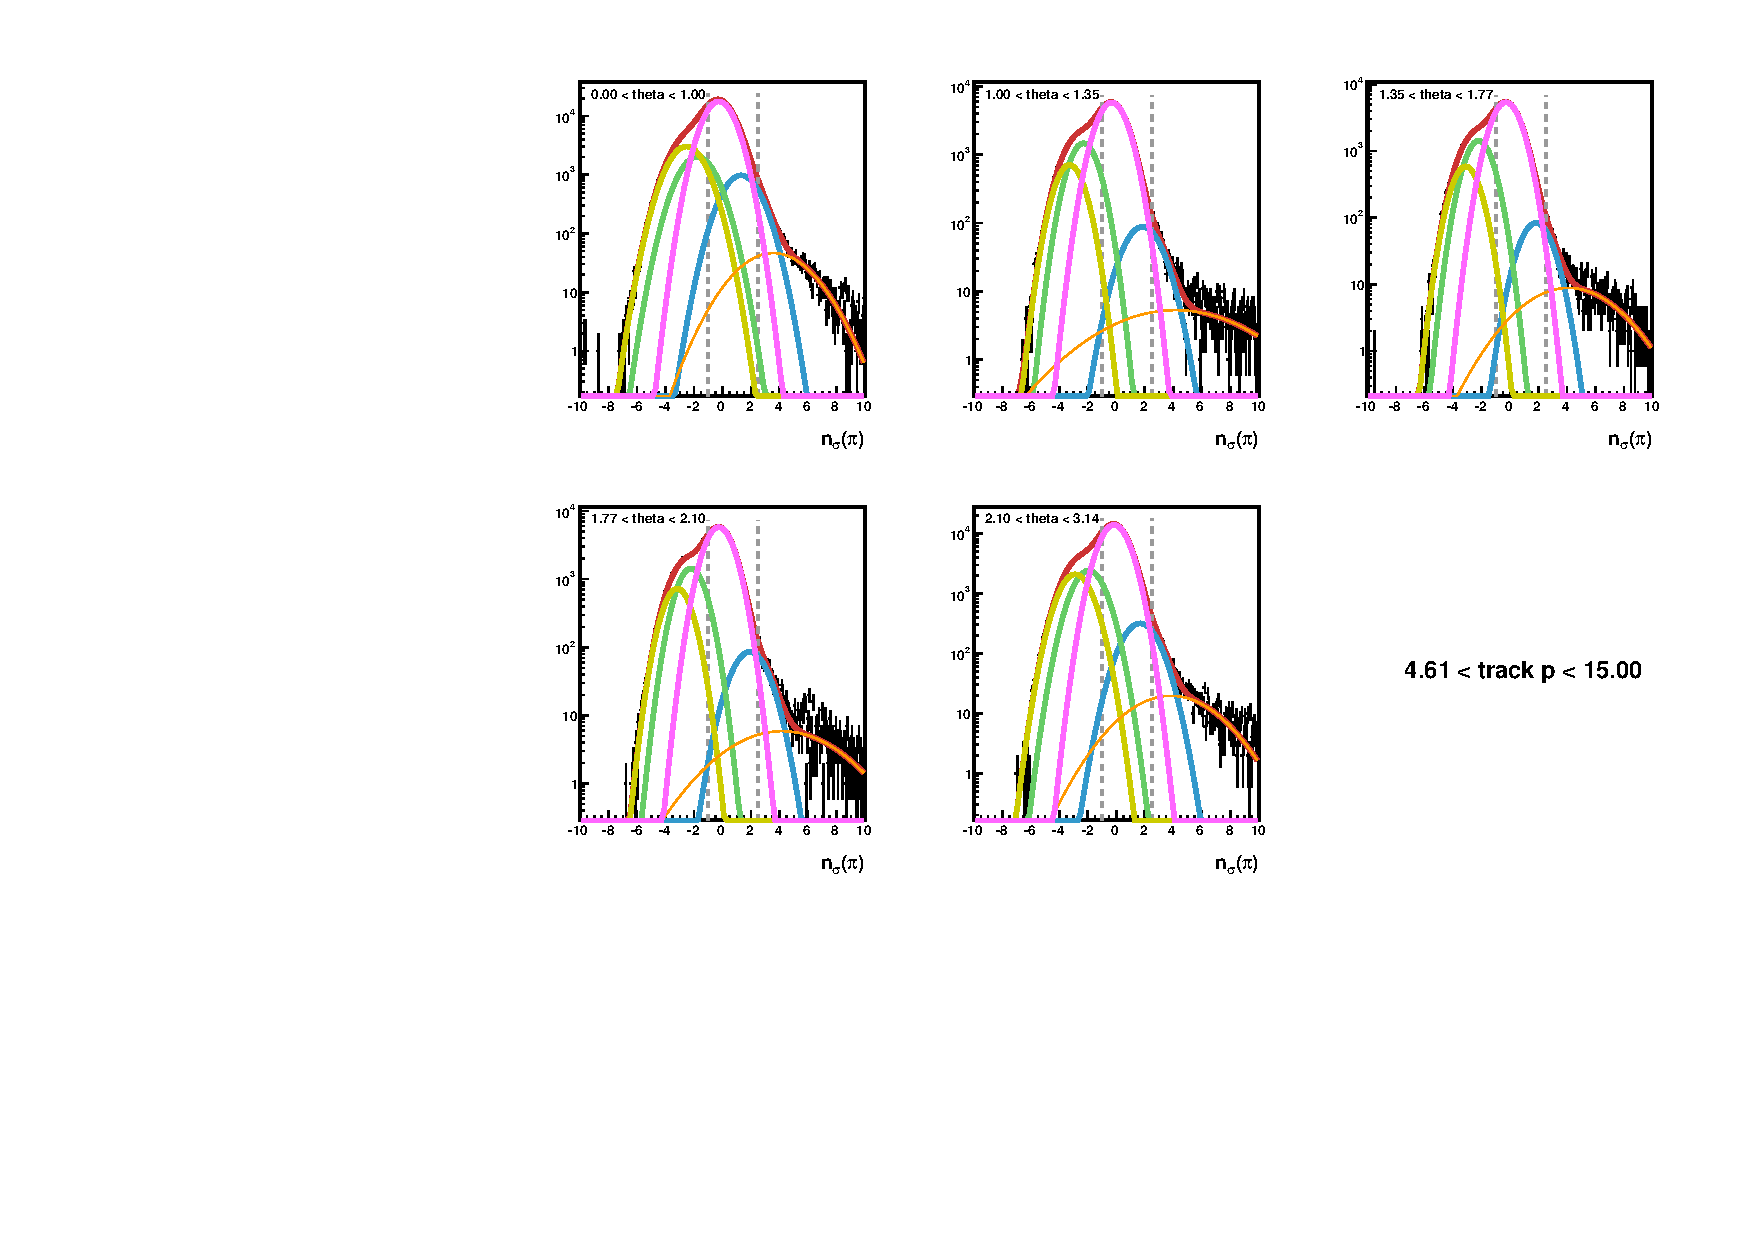
\includegraphics[width = .7\textwidth]{5gausFit_pbin_4.pdf}
\caption[]{}
\label{fig:5gaus4}
\end{center}
\end{figure}

 \begin{figure}
\begin{center}
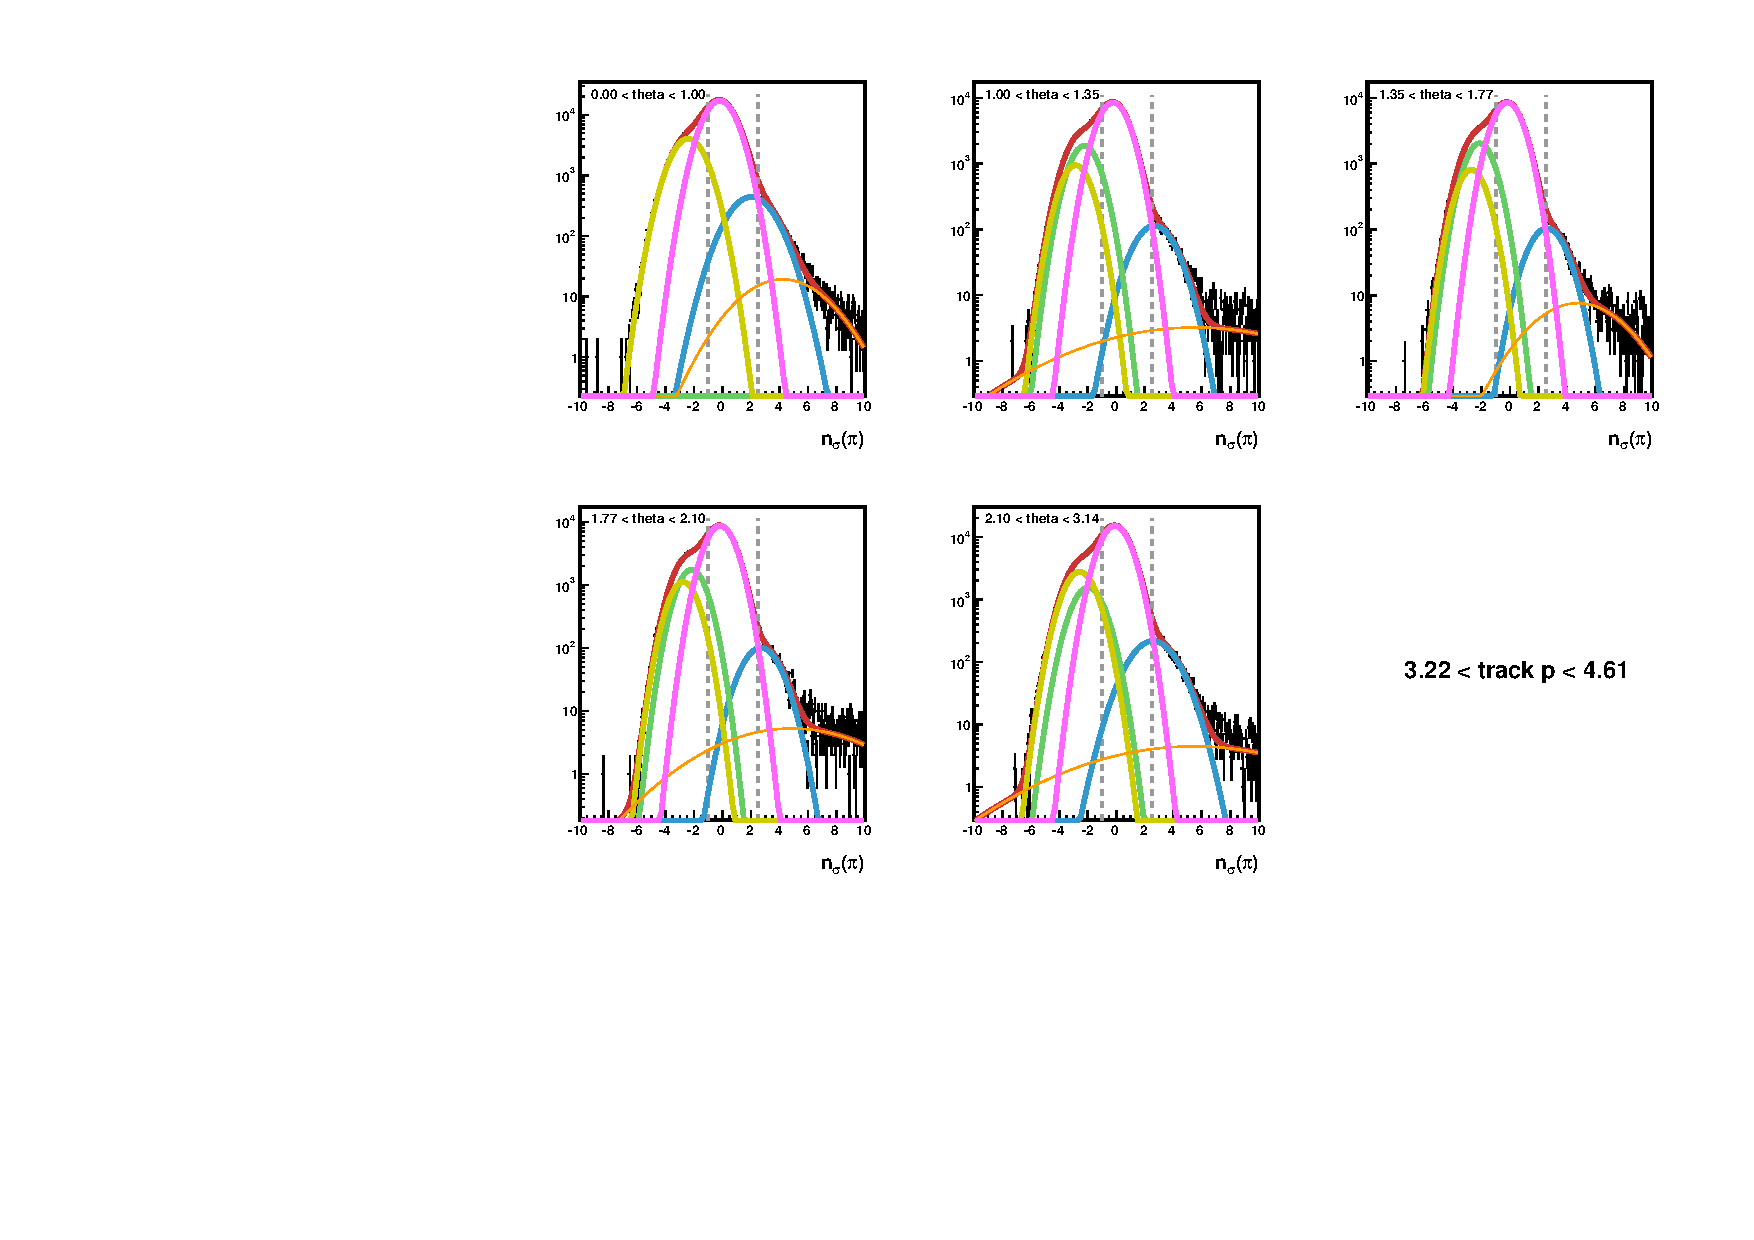
\includegraphics[width = .7\textwidth]{5gausFit_pbin_3.pdf}
\caption[]{}
\label{fig:5gaus3}
\end{center}
\end{figure}

 \begin{figure}
\begin{center}
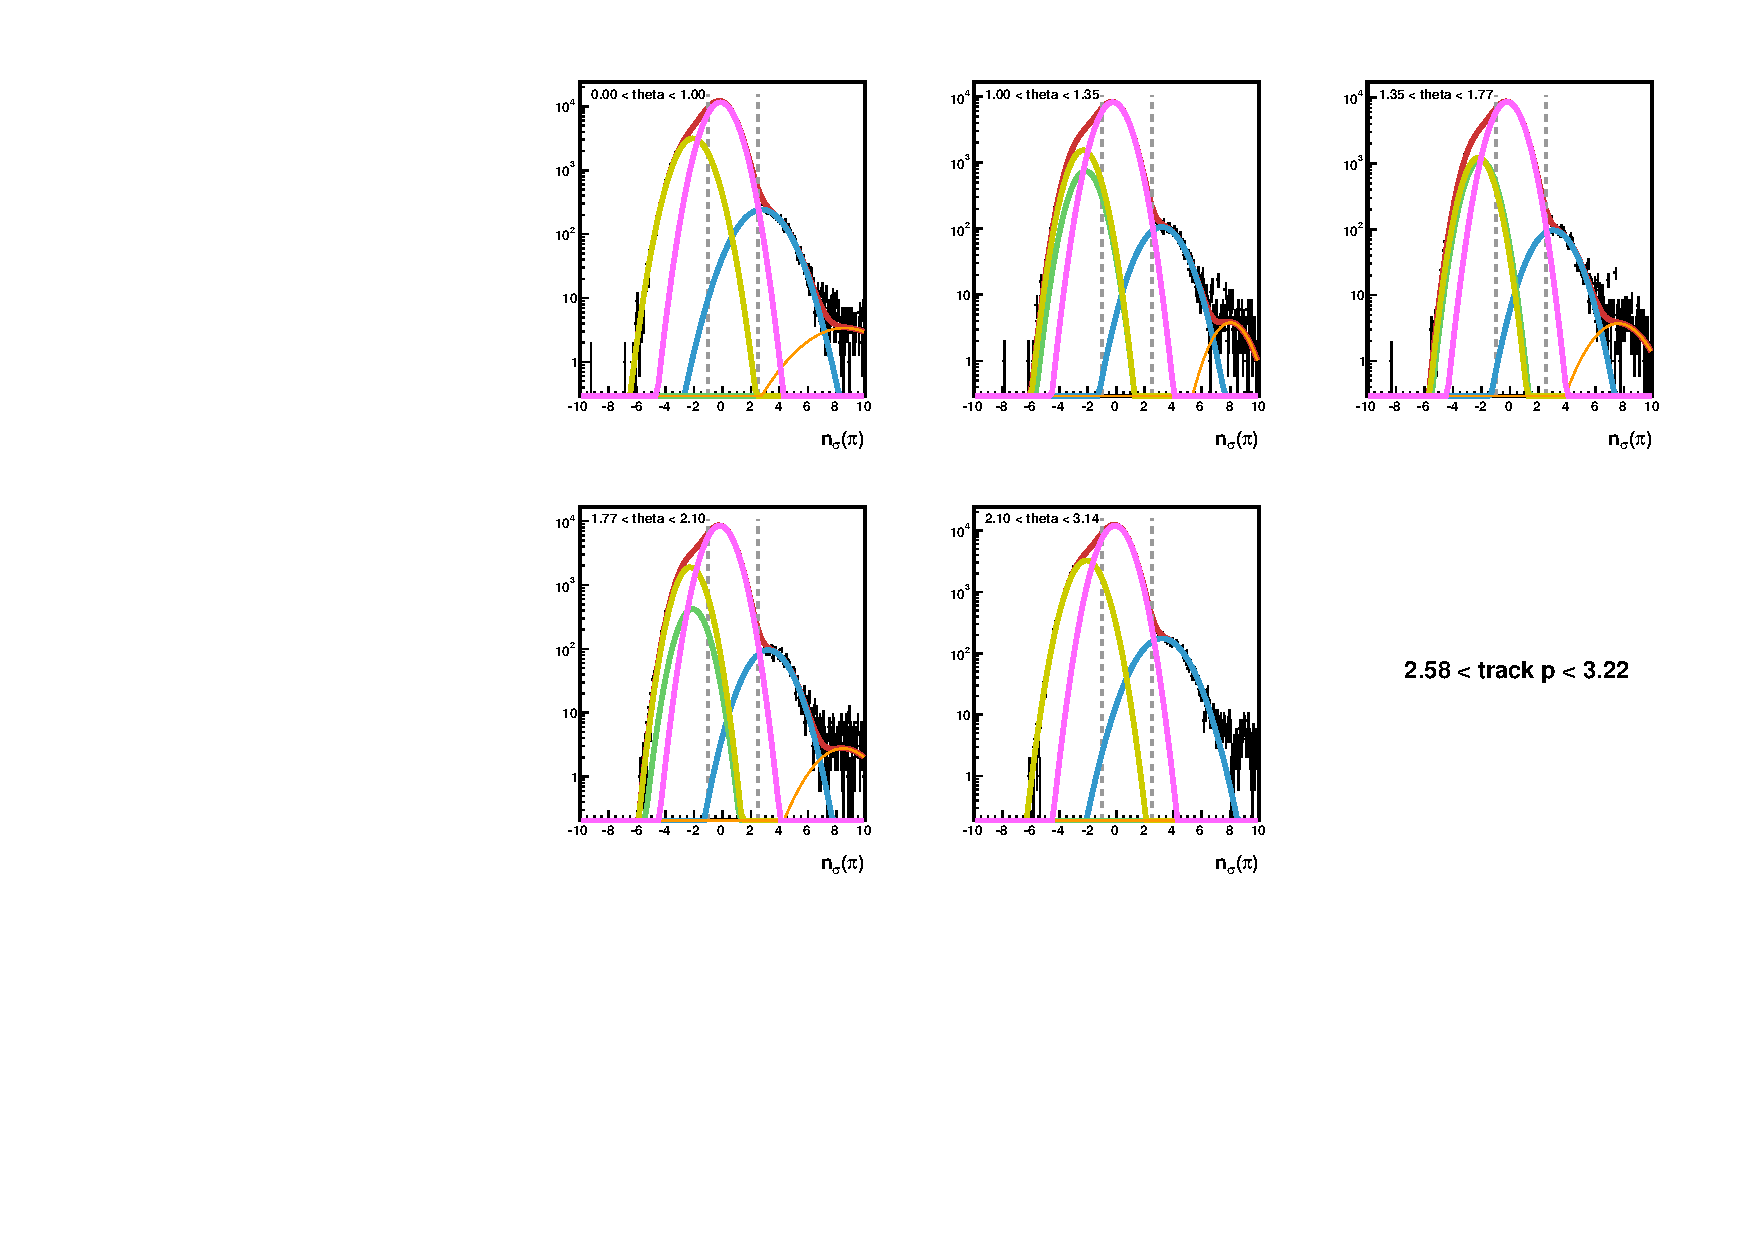
\includegraphics[width = .7\textwidth]{5gausFit_pbin_2.pdf}
\caption[]{}
\label{fig:5gaus2}
\end{center}
\end{figure}

 \begin{figure}
\begin{center}
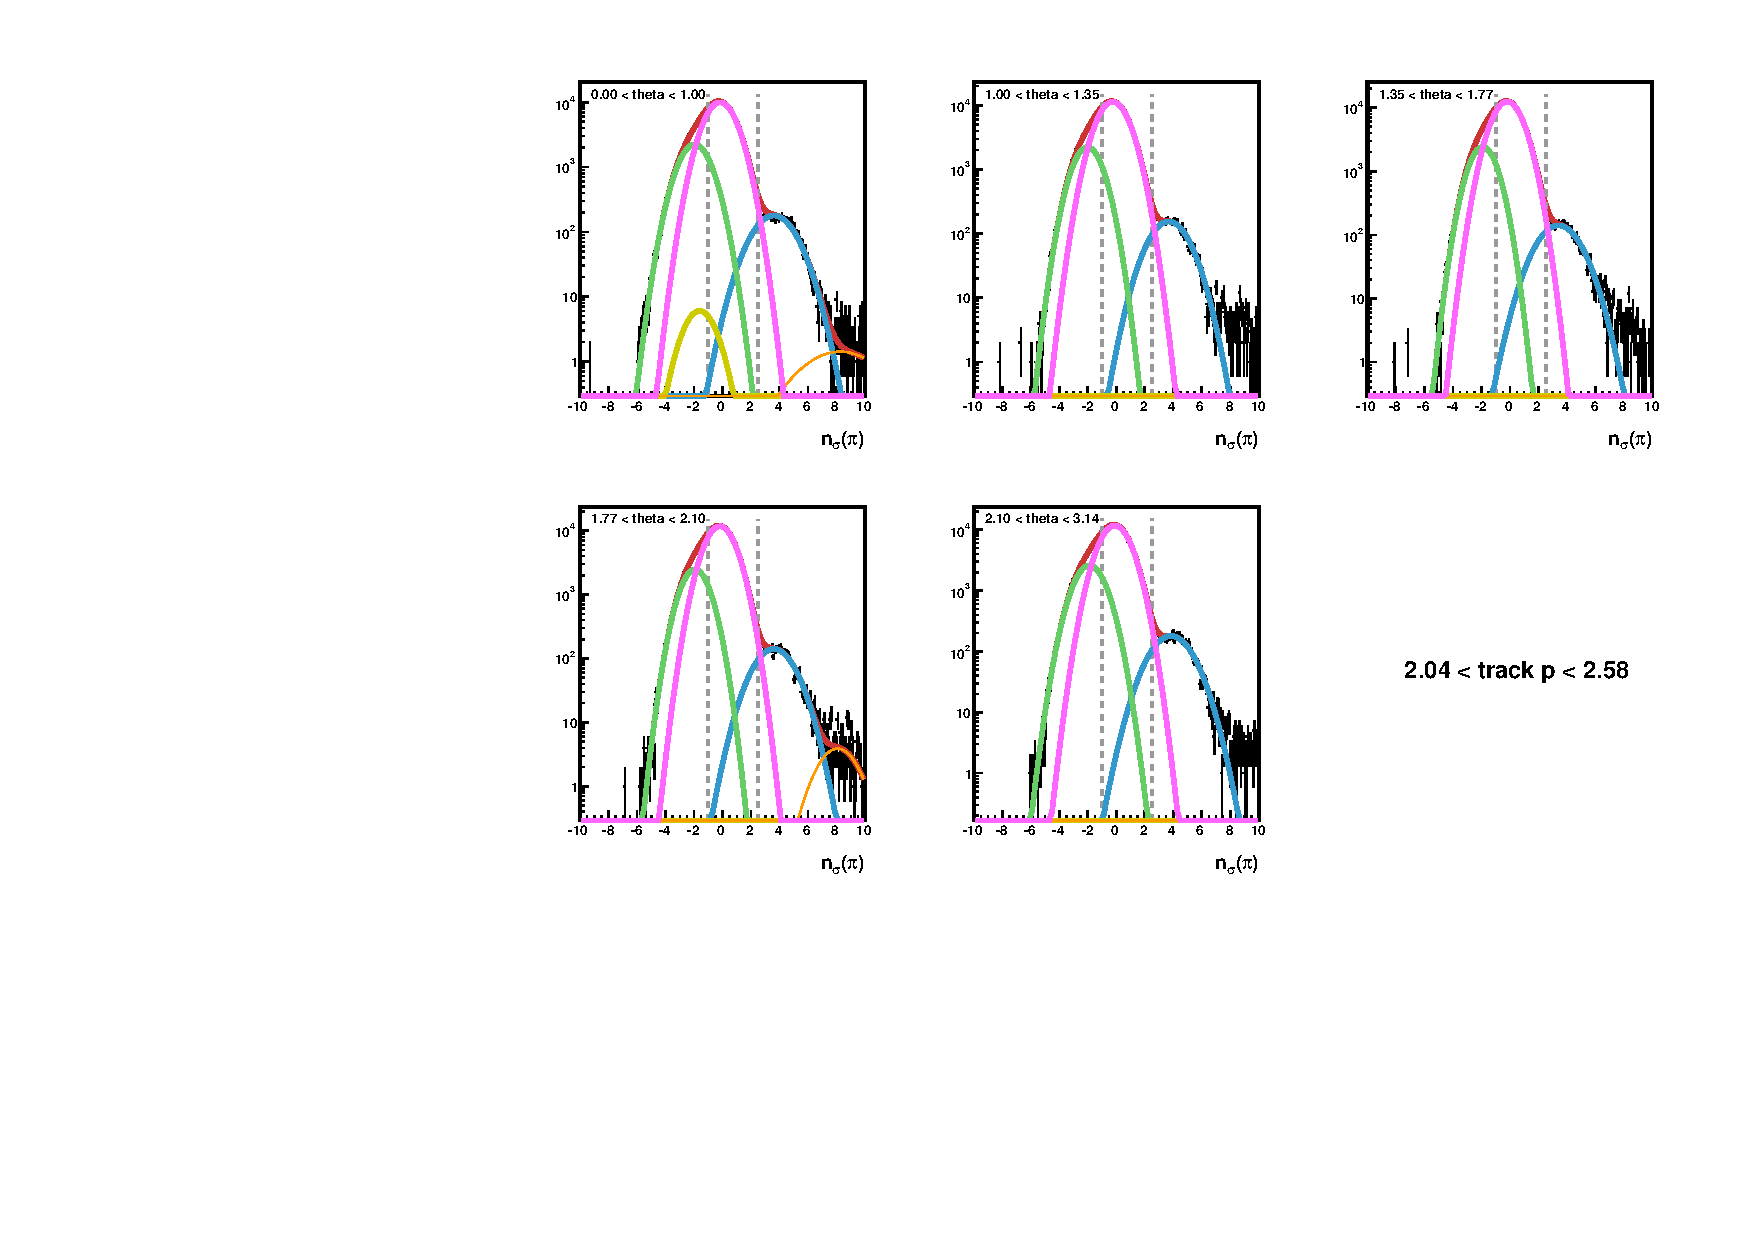
\includegraphics[width = .7\textwidth]{5gausFit_pbin_1.pdf}
\caption[]{}
\label{fig:5gaus1}
\end{center}
\end{figure}

 \begin{figure}
\begin{center}
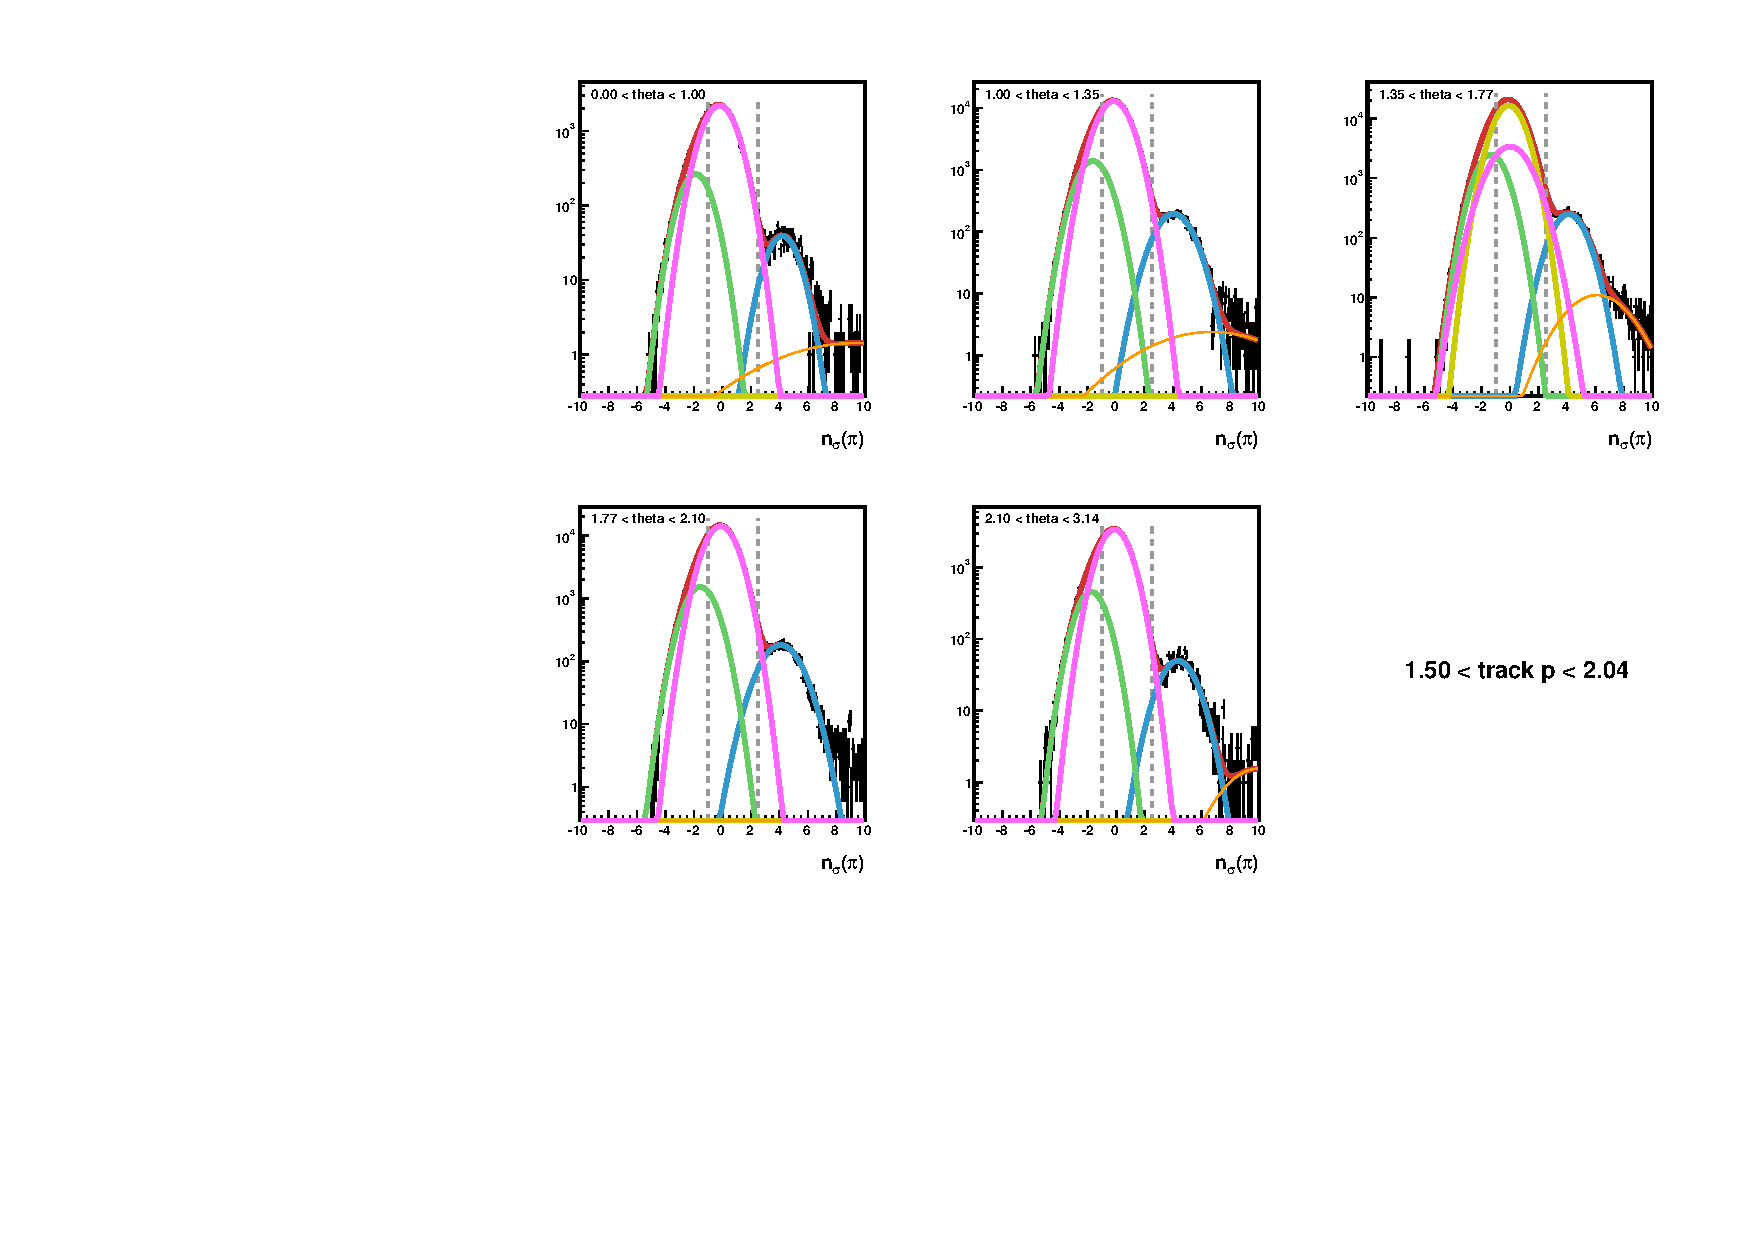
\includegraphics[width = .7\textwidth]{5gausFit_pbin_0.pdf}
\caption[]{}
\label{fig:5gaus0}
\end{center}
\end{figure}

 \begin{figure}
\begin{center}
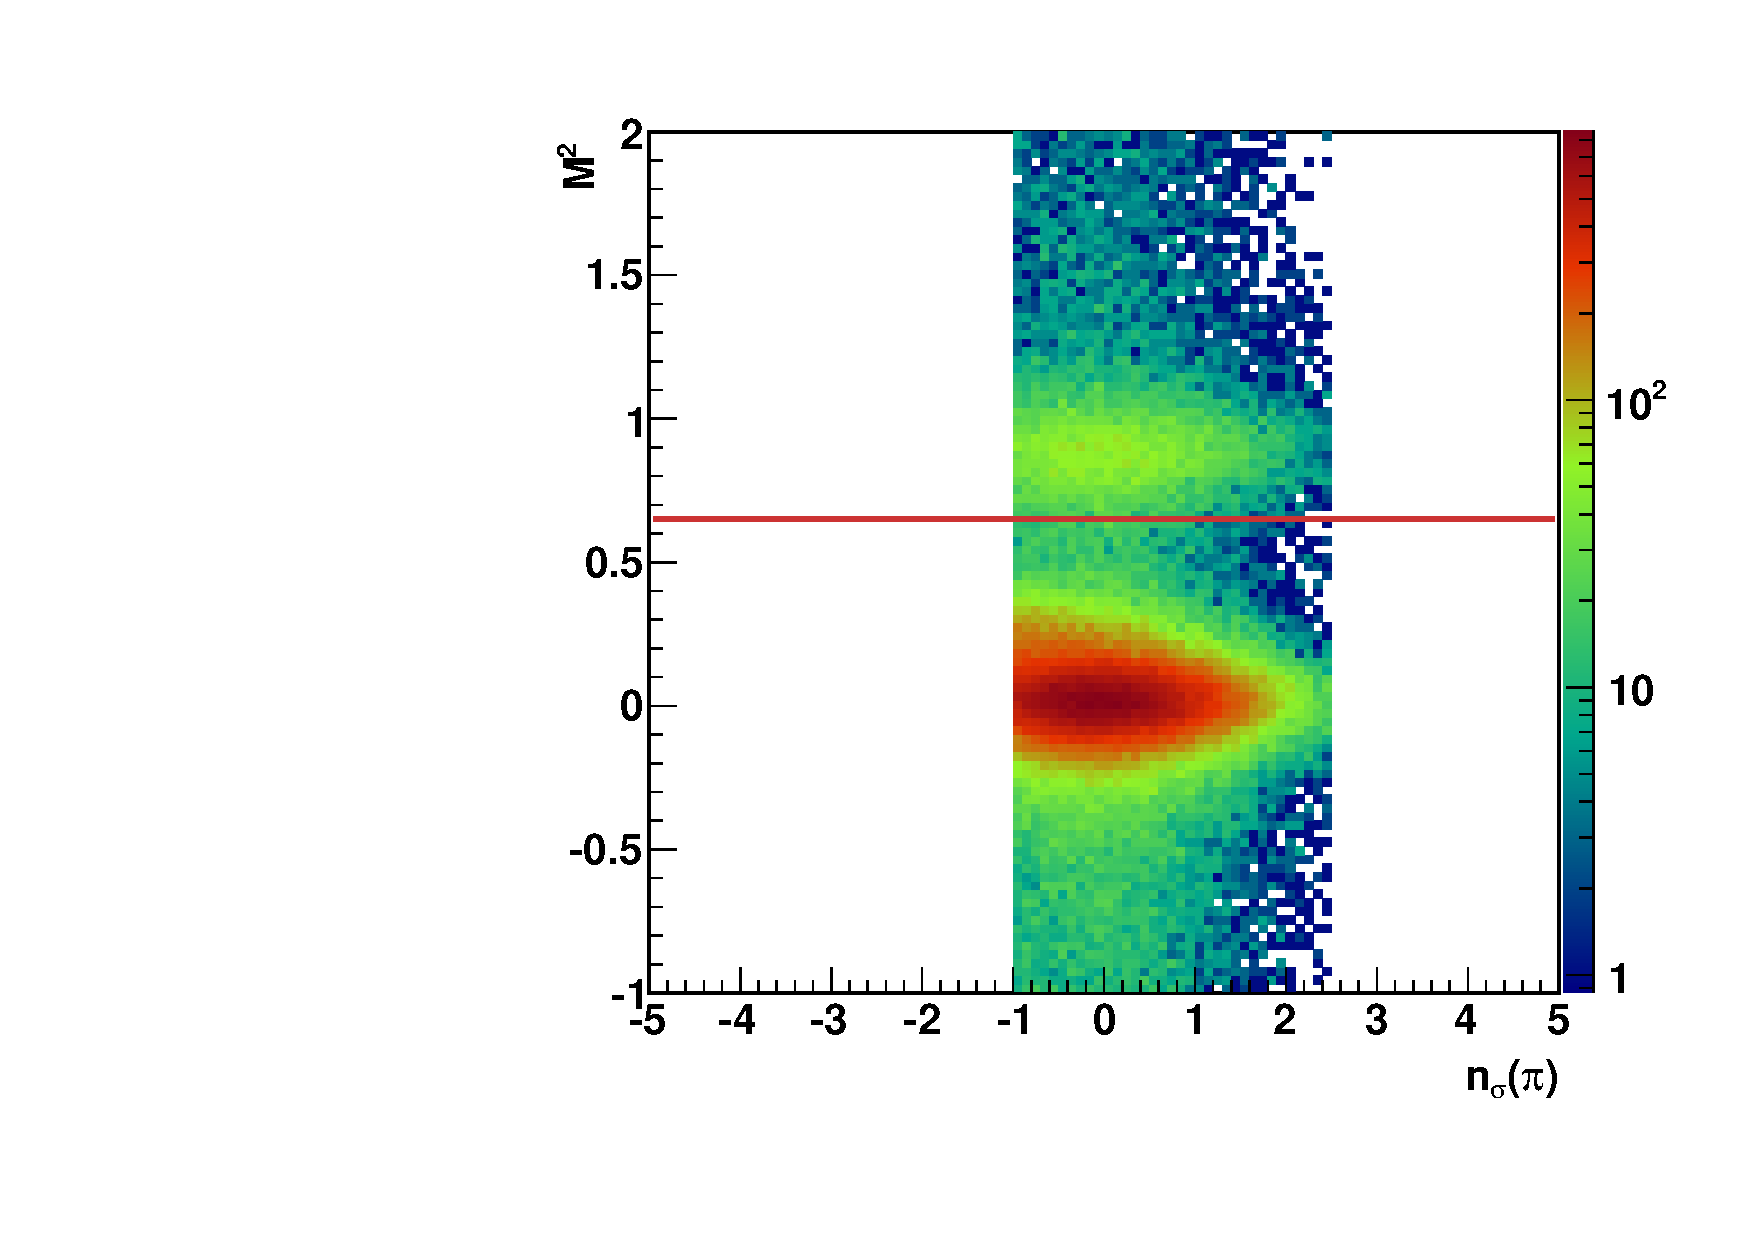
\includegraphics[width = .7\textwidth]{tofPlot.pdf}
\caption[]{}
\label{fig:tofPlot}
\end{center}
\end{figure}





\section{Finding $\pi^+\pi^-$ Pairs}
\begin{figure}
\begin{center}
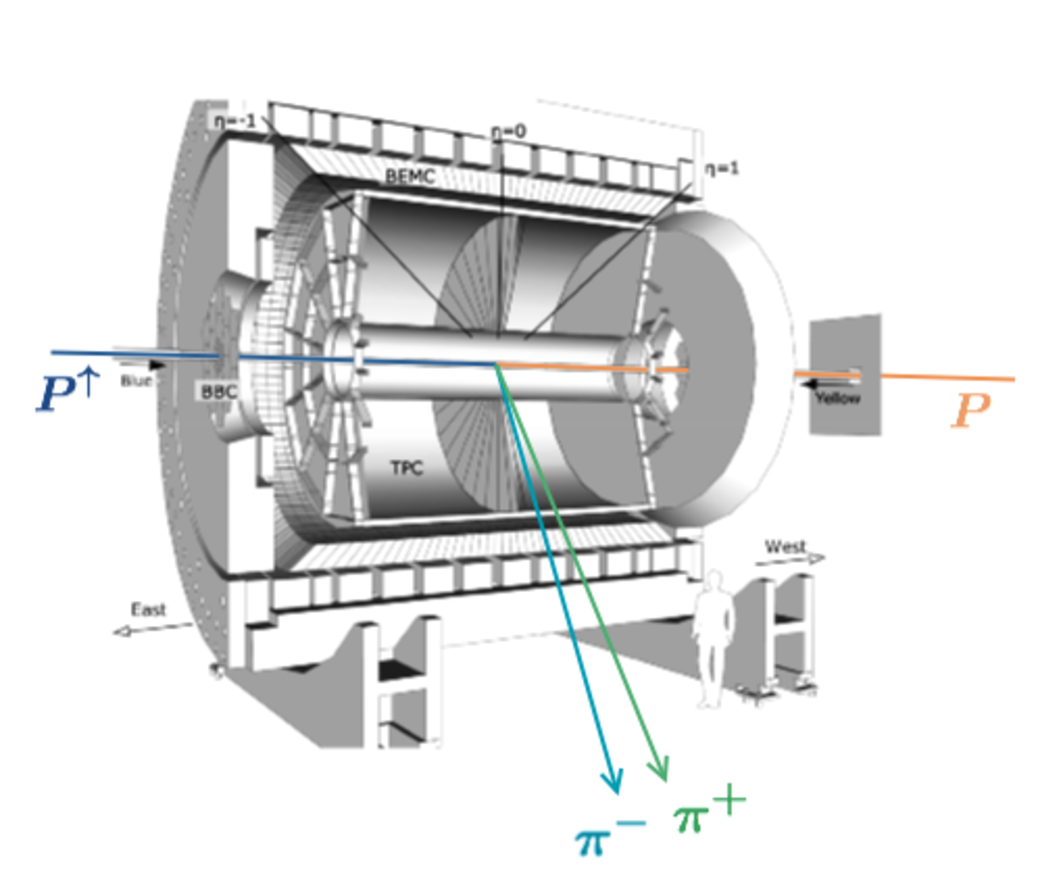
\includegraphics[width = .7\textwidth]{starPic6}
\caption[Schematic of Analysis]{}
\label{fig:analSchem}
\end{center}
\end{figure}


The first step in finding pion pairs is to select events which are worth looking at. We do this by only concentrating on events which trigger at least one of the following STAR triggers: JP0, JP1, JP2, AJP, BHT0VPD, BHT1VPD, BHT2BBC, or BHT2. Selecting our data based on these triggers introduces a bias to our sample. The effect of this biasing will be discussed in detail in chapeter ADD CHAPTER NUMBER FOR 2012 SIMULATION ANALYSIS.

For every event pions are identified by ionization energy loss in the TPC. A value, $n_\sigma(\pi)$, is given to each track in an event describing how many standard deviations away it is from an ideal pion on the ionization energy loss curve shown in figure \ref{fig:dedx}. If there were only pions, the distribution of $n_\sigma(\pi)$ values would be normal centered around 0. However as you can see in figure \ref{fig:nSigPiCut}, the red curve is not a gaussian. This is due to contamination from kaons/protons and electrons. To account for this we fit the $n_\sigma(\pi)$ distribution with three gaussians. The purple curve centered around zero is what we consider pions, the green curve centered at -2 are kaons and protons, and the small blue curve at about 3 is electrons. A clean sample of pions can be found by selecting tracks with an $n_\sigma(\pi)$ between -1 and 2.5. This is shown by the vertical orange lines in figure \ref{fig:nSigPiCut}. This choice of an $n_\sigma(\pi)$ range avoids the kaon-proton peak while still allowing the majority of pions. Figure  \ref{fig:contamination} shows the contamination from kaons, protons, and electrons for different $\eta^{\pi^+\pi^-}$.

\begin{figure}
\begin{center}
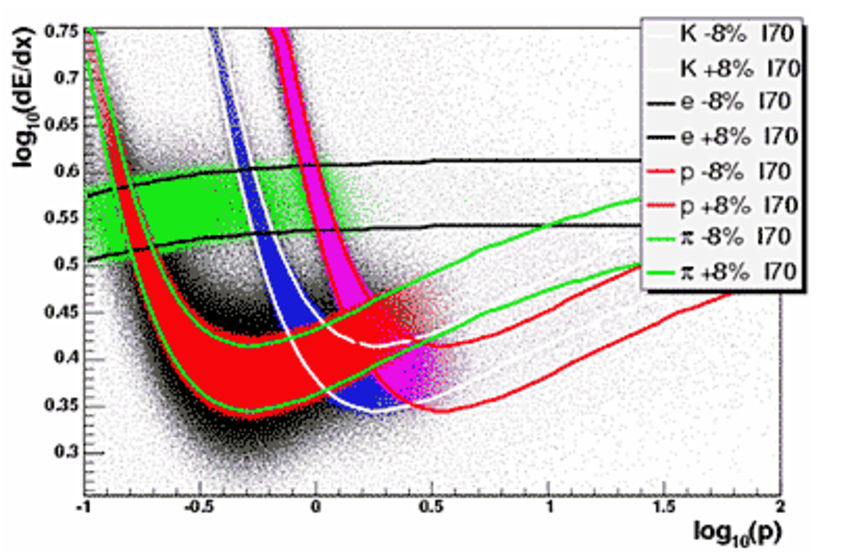
\includegraphics[width = 1\textwidth]{dedxforPID}
\caption[Ionization energy loss in TPC gas on log scale]{ionization energy loss vs momentum in TPC. Tracks in the red band are pions we want to find. The blue and pink band are koans and protons we want minimize in our sample}
\label{fig:dedx}
\end{center}
\end{figure}


\begin{figure}
\begin{center}
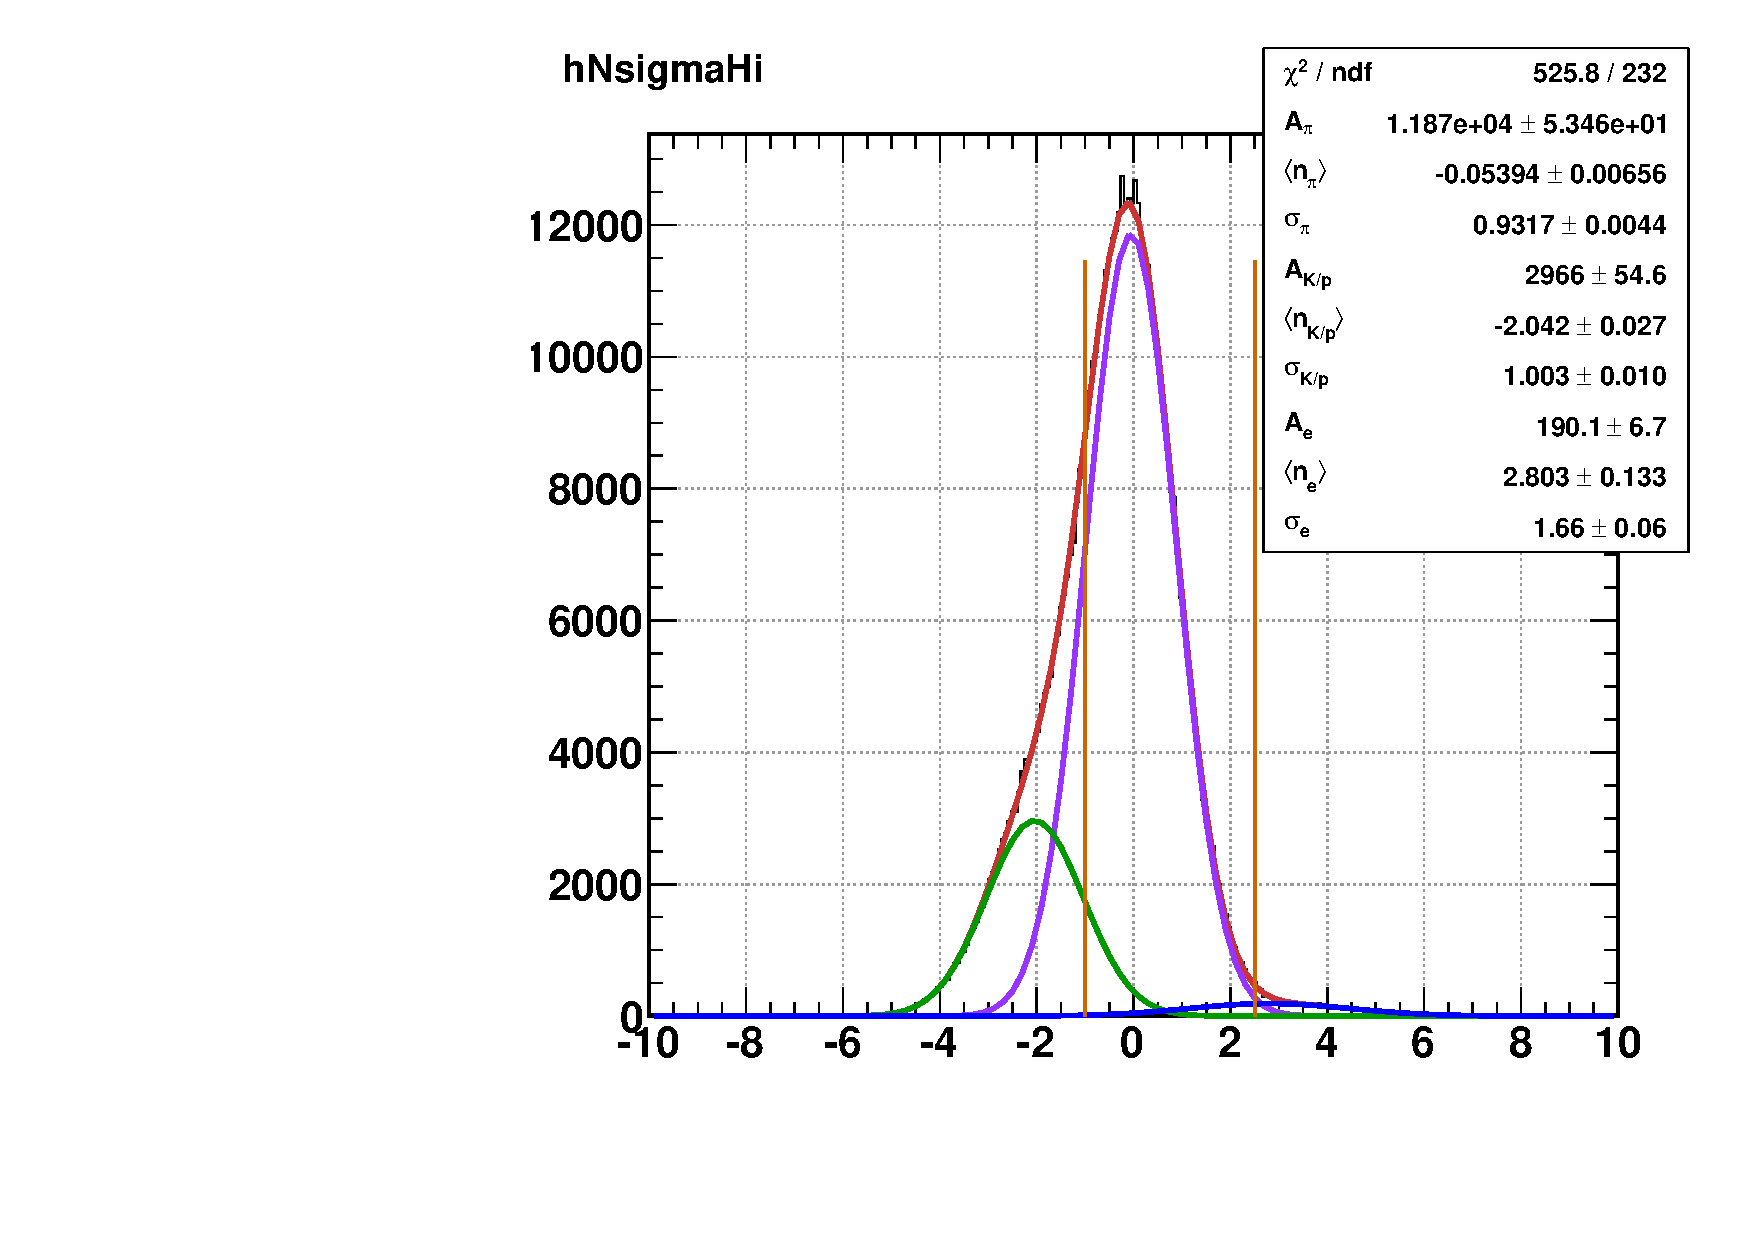
\includegraphics[width = 1\textwidth]{nSigma_05_1}
\caption[$\nsigpi$ distribution and tripple Gaussian fit]{Distribution of $\nsigpi$ fit with three Gaussians.}
\label{fig:nSigPiCut}
\end{center}
\end{figure}

\begin{figure}
\begin{center}
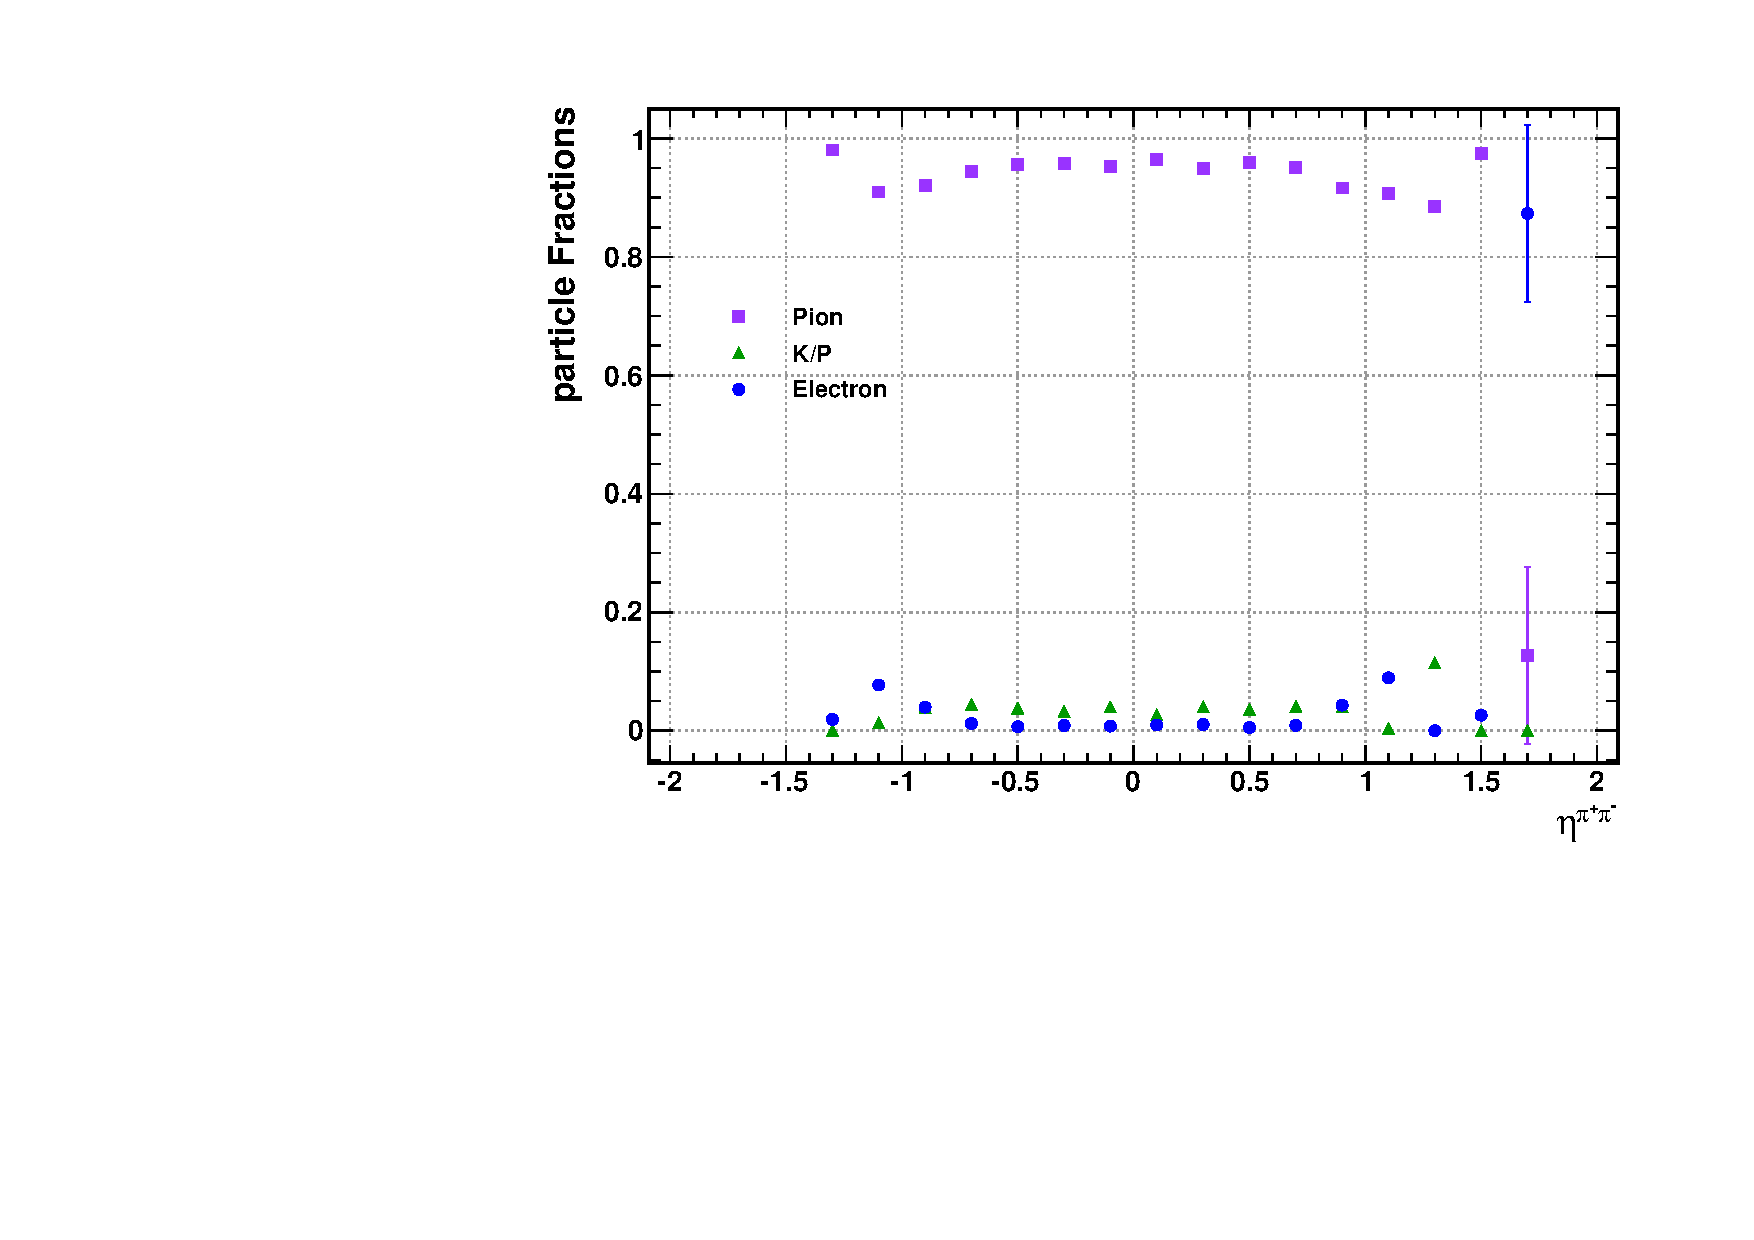
\includegraphics[width = 1\textwidth]{nSigmaVsEta_witherrors.pdf}
\caption[Contamination of pion sample]{contamination from kaon, proton, and electron}
\label{fig:contamination}
\end{center}
\end{figure}

Once a clean sample is found $\pi^+$s and $\pi^-$s must be combined into $\pi^+\pi^-$ pairs. Every combination of $\pi^+$ and $\pi^-$ in an event are checked. They become a pair if they pass the individual track cuts and if they are contained in a cone of a certain radius in $\eta-\phi$ space (figure). For 1D binning, radii of 0.2, 0.3, and 0.4 are while 0.7 is used in 2D binning in order to increase statistics.  

\begin{figure}
\begin{center}
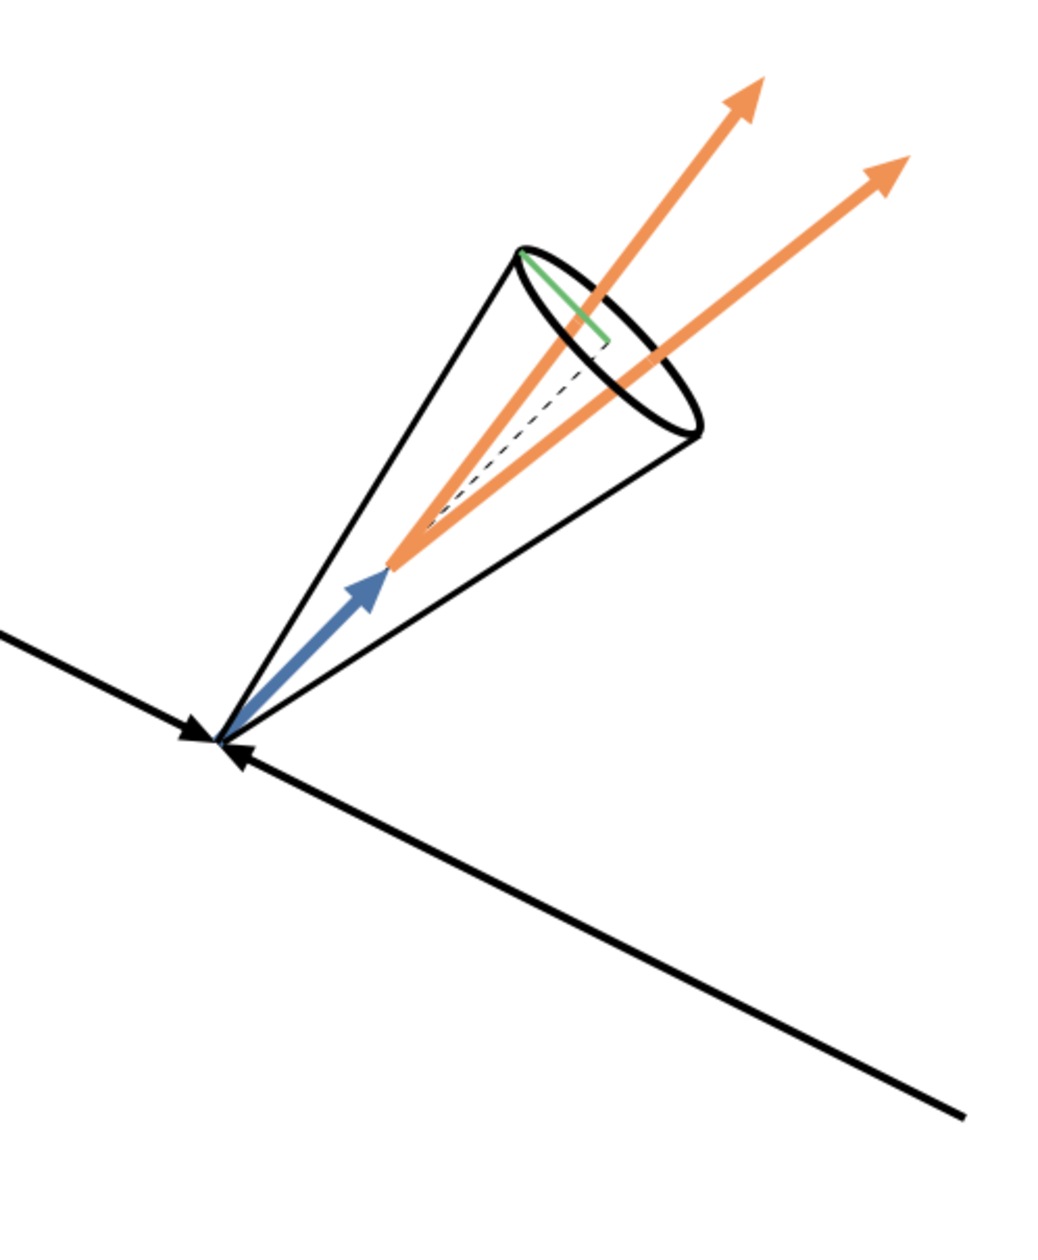
\includegraphics[width = 1\textwidth]{coneNew3}
\caption[Radius cut]{radius cut}
\label{fig:radCut}
\end{center}
\end{figure}

\FloatBarrier
\section{Pair Distributions}

The entire data set provides 17544516 $\pi^+\pi^-$ pairs in a radius between 0.05 and 1.0 in $\eta,\phi$ space before trigger information is used. The minimum radius cut of 0.05 is used because when the tracks are very close together, the uncertainty in track position can cause the orientation of the pairs to flip. 


Once the data set was ready, quality tests were preformed on the pion pairs. These included looking at the invariant mass, transverse momentum, and pseudorapidity distributions for the pairs. Quality control plots of relevant kinematic variables of individual pions and pion pairs can be seen in figures \ref{fig:posPt} to \ref{fig:cosTheta}. 


\begin{figure}
\begin{center}
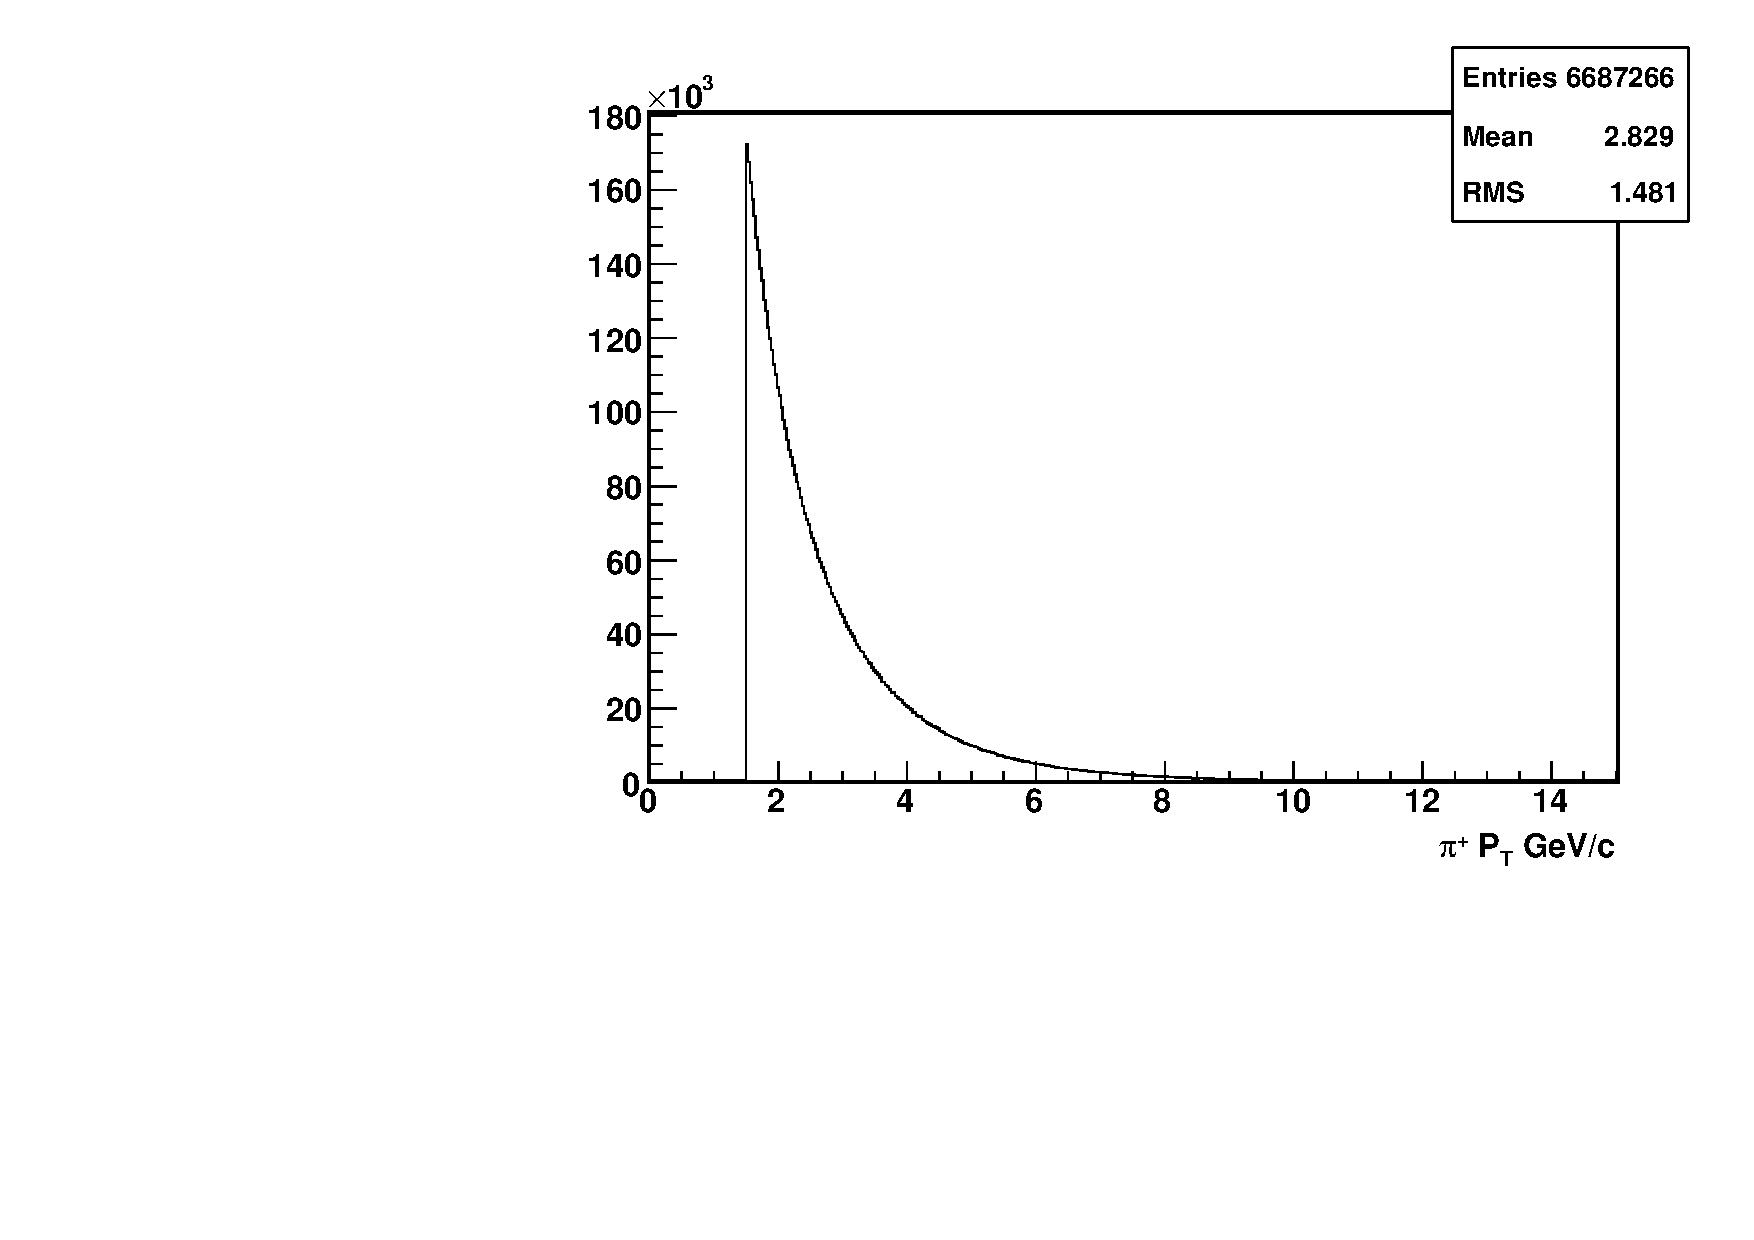
\includegraphics[width = .8\textwidth]{hPosPt}
\caption[$P_{T}$ distribution of $\pi^+$]{}
\label{fig:posPt}
\end{center}
\end{figure}

\begin{figure}
\begin{center}
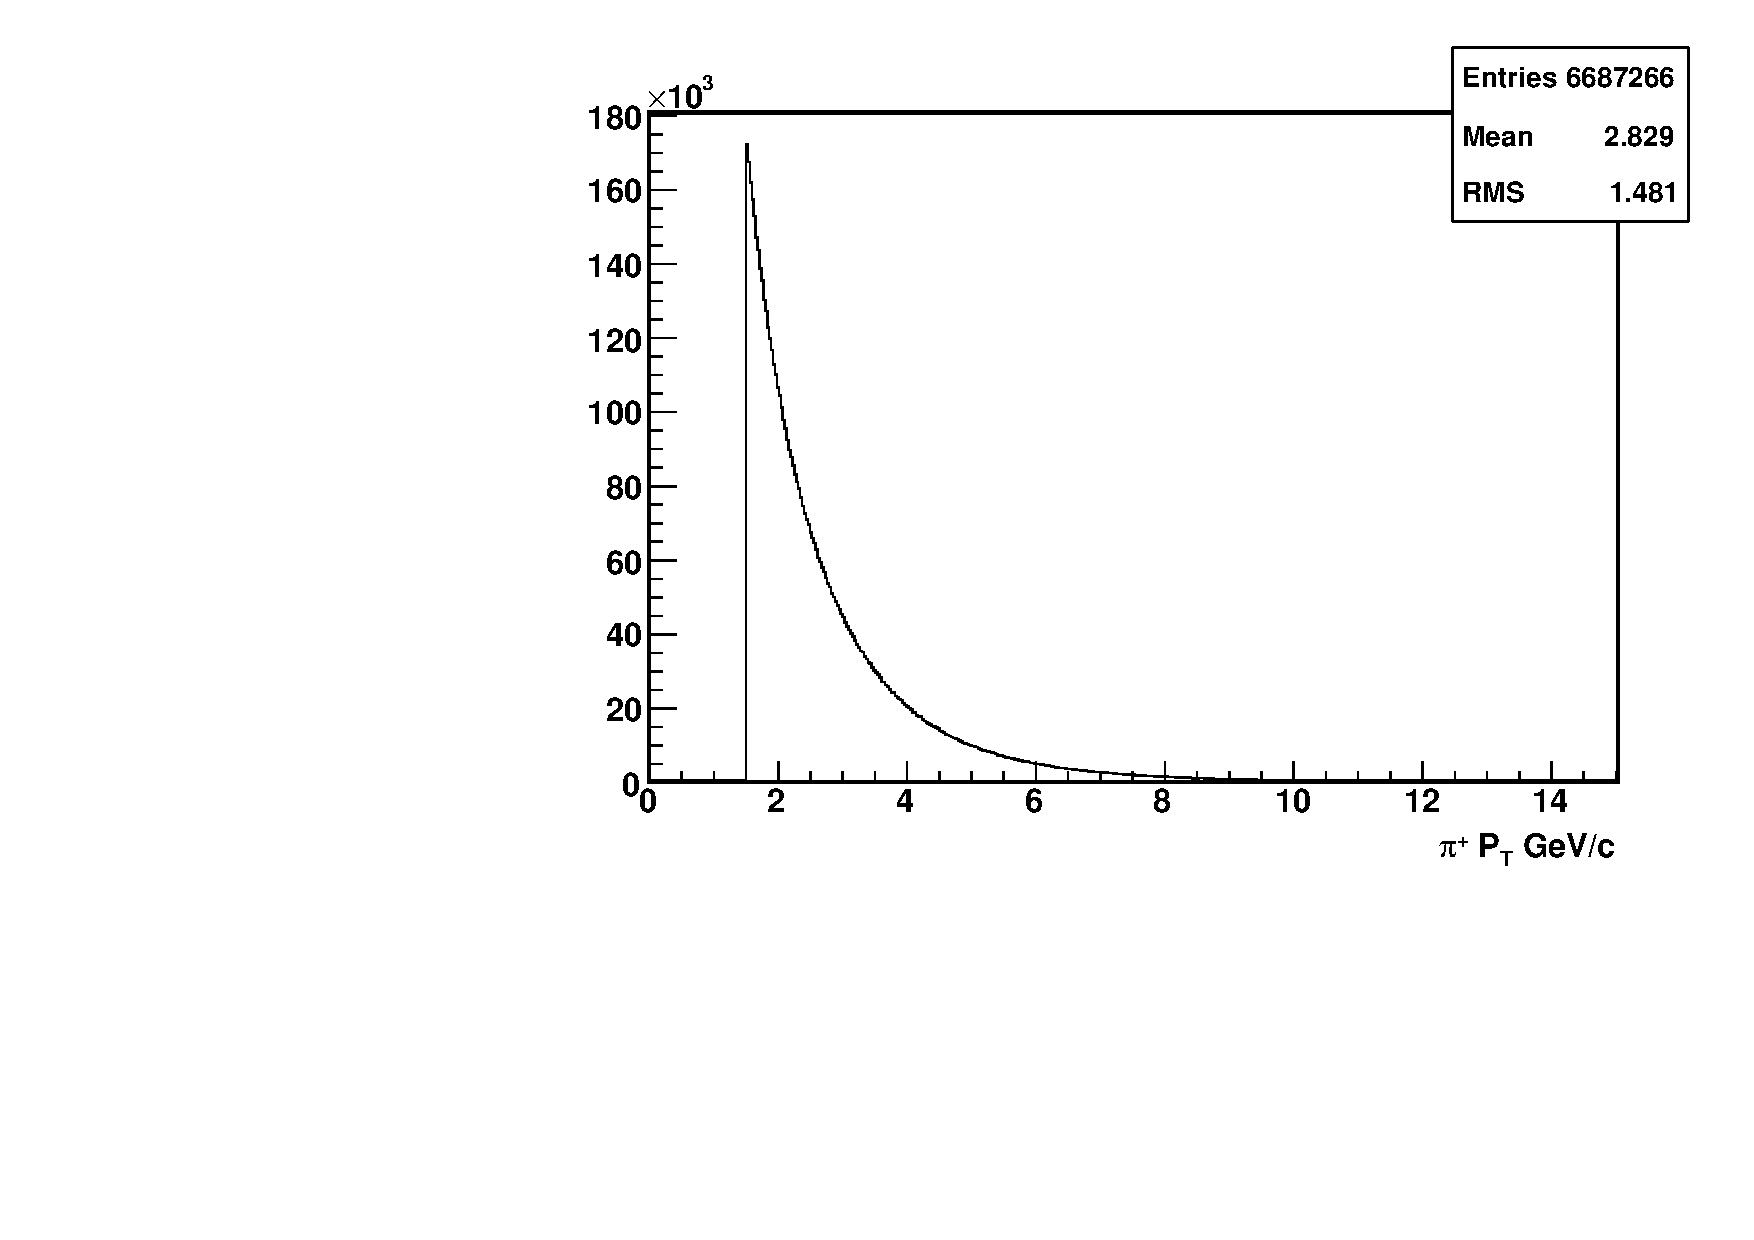
\includegraphics[width = .8\textwidth]{hNegPt}
\caption[$P_{T}$ distribution of $\pi^-$]{}
\label{fig:}
\end{center}
\end{figure}

\begin{figure}
\begin{center}
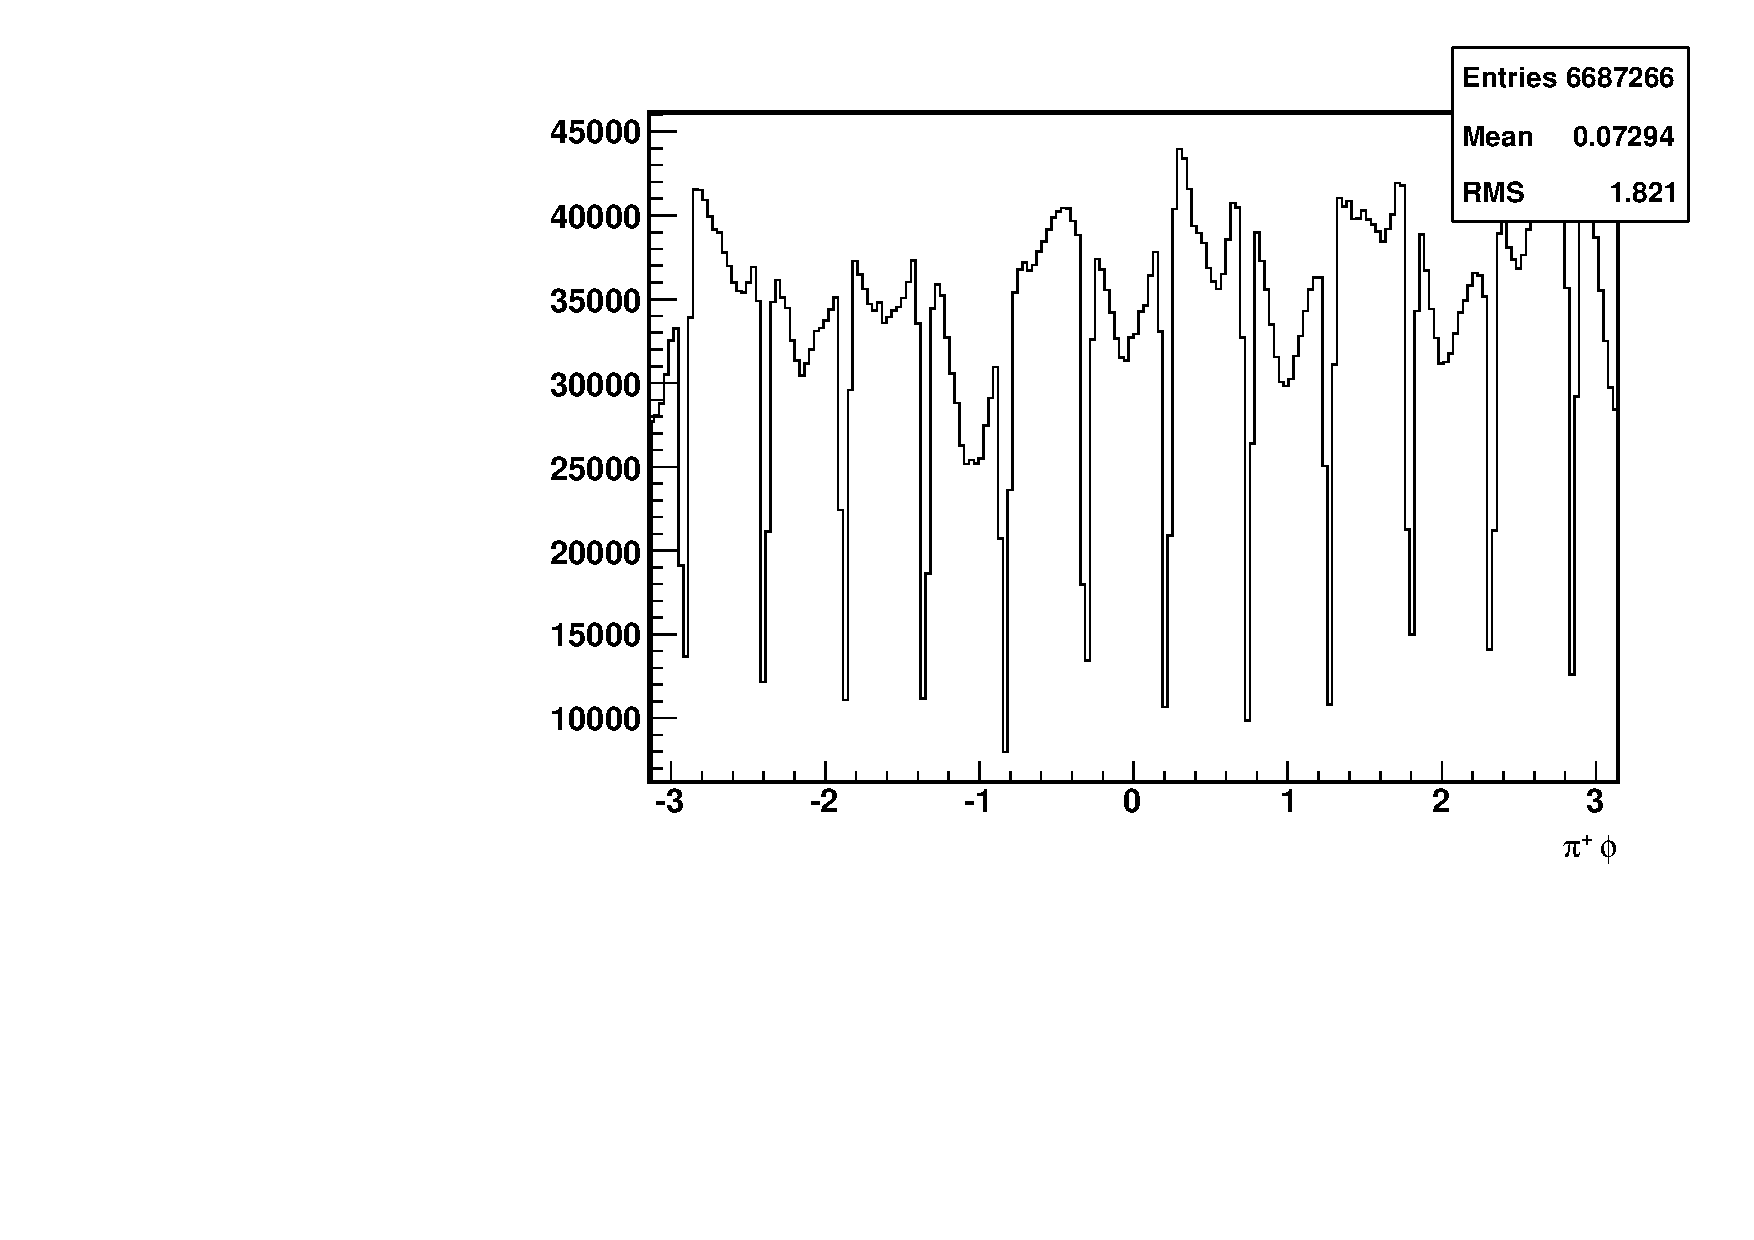
\includegraphics[width = .8\textwidth]{hPosPhi}
\caption[$\phi$ distribution of $\pi^+$]{}
\label{fig:}
\end{center}
\end{figure}

\begin{figure}
\begin{center}
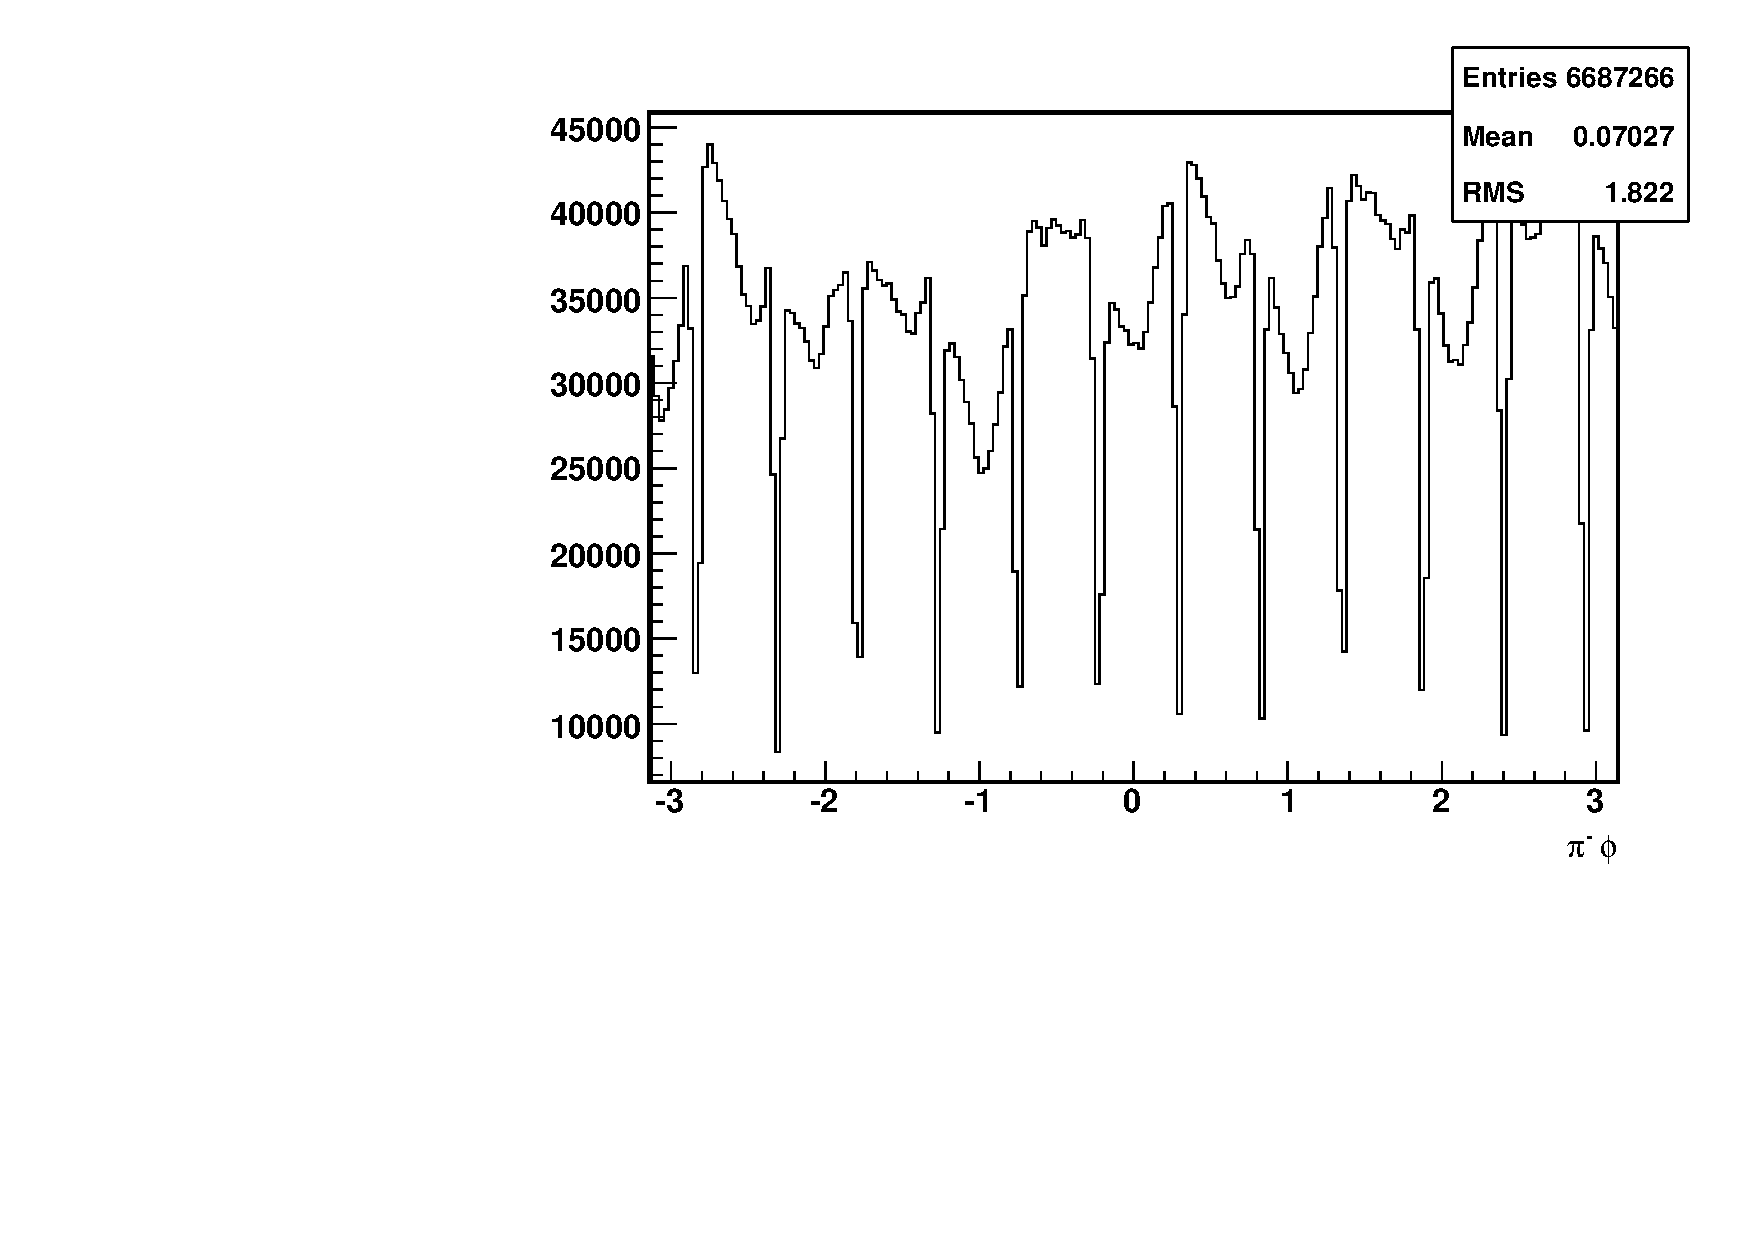
\includegraphics[width = .8\textwidth]{hNegPhi}
\caption[$\phi$ distribution of $\pi^-$]{}
\label{fig:}
\end{center}
\end{figure}

\begin{figure}
\begin{center}
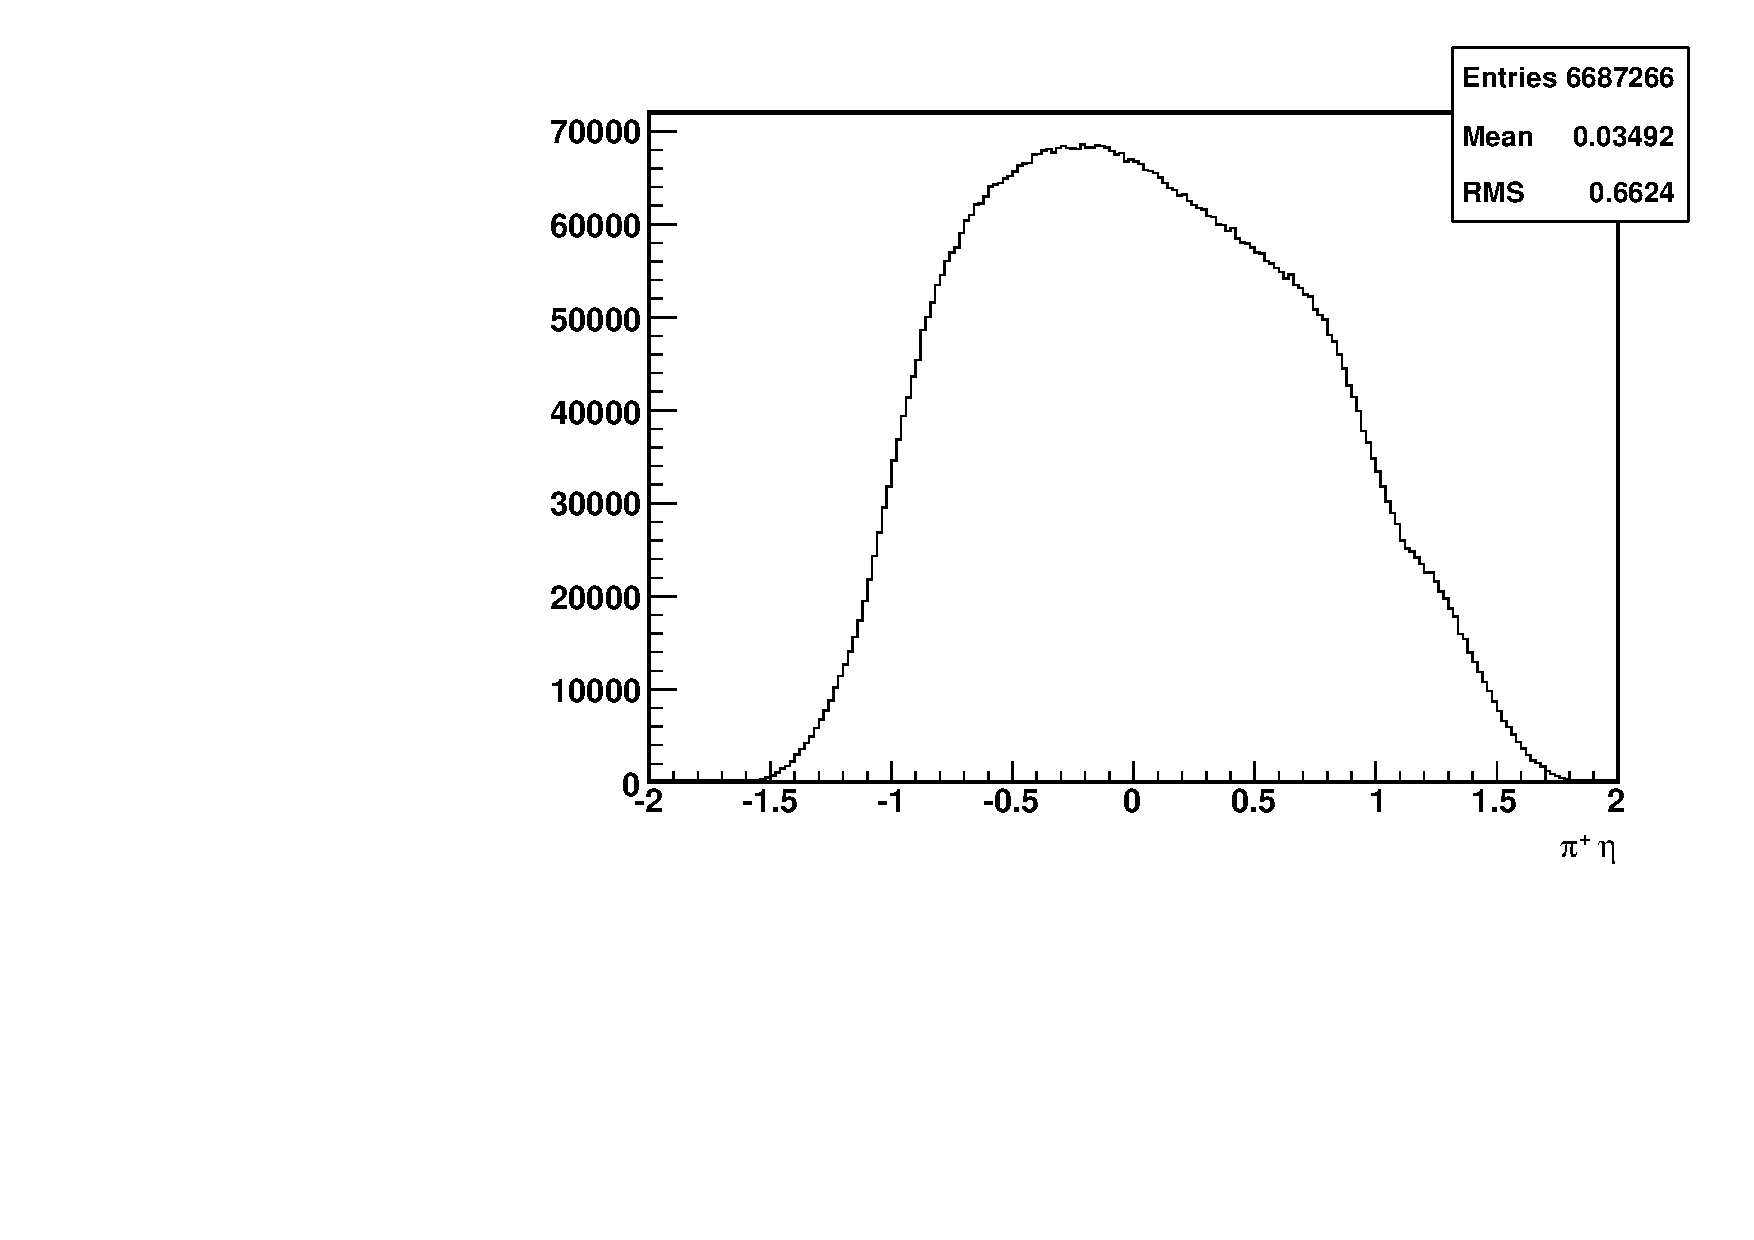
\includegraphics[width = .8\textwidth]{hPosEta}
\caption[$\eta$ distribution of $\pi^+$]{}
\label{fig:}
\end{center}
\end{figure}

\begin{figure}
\begin{center}
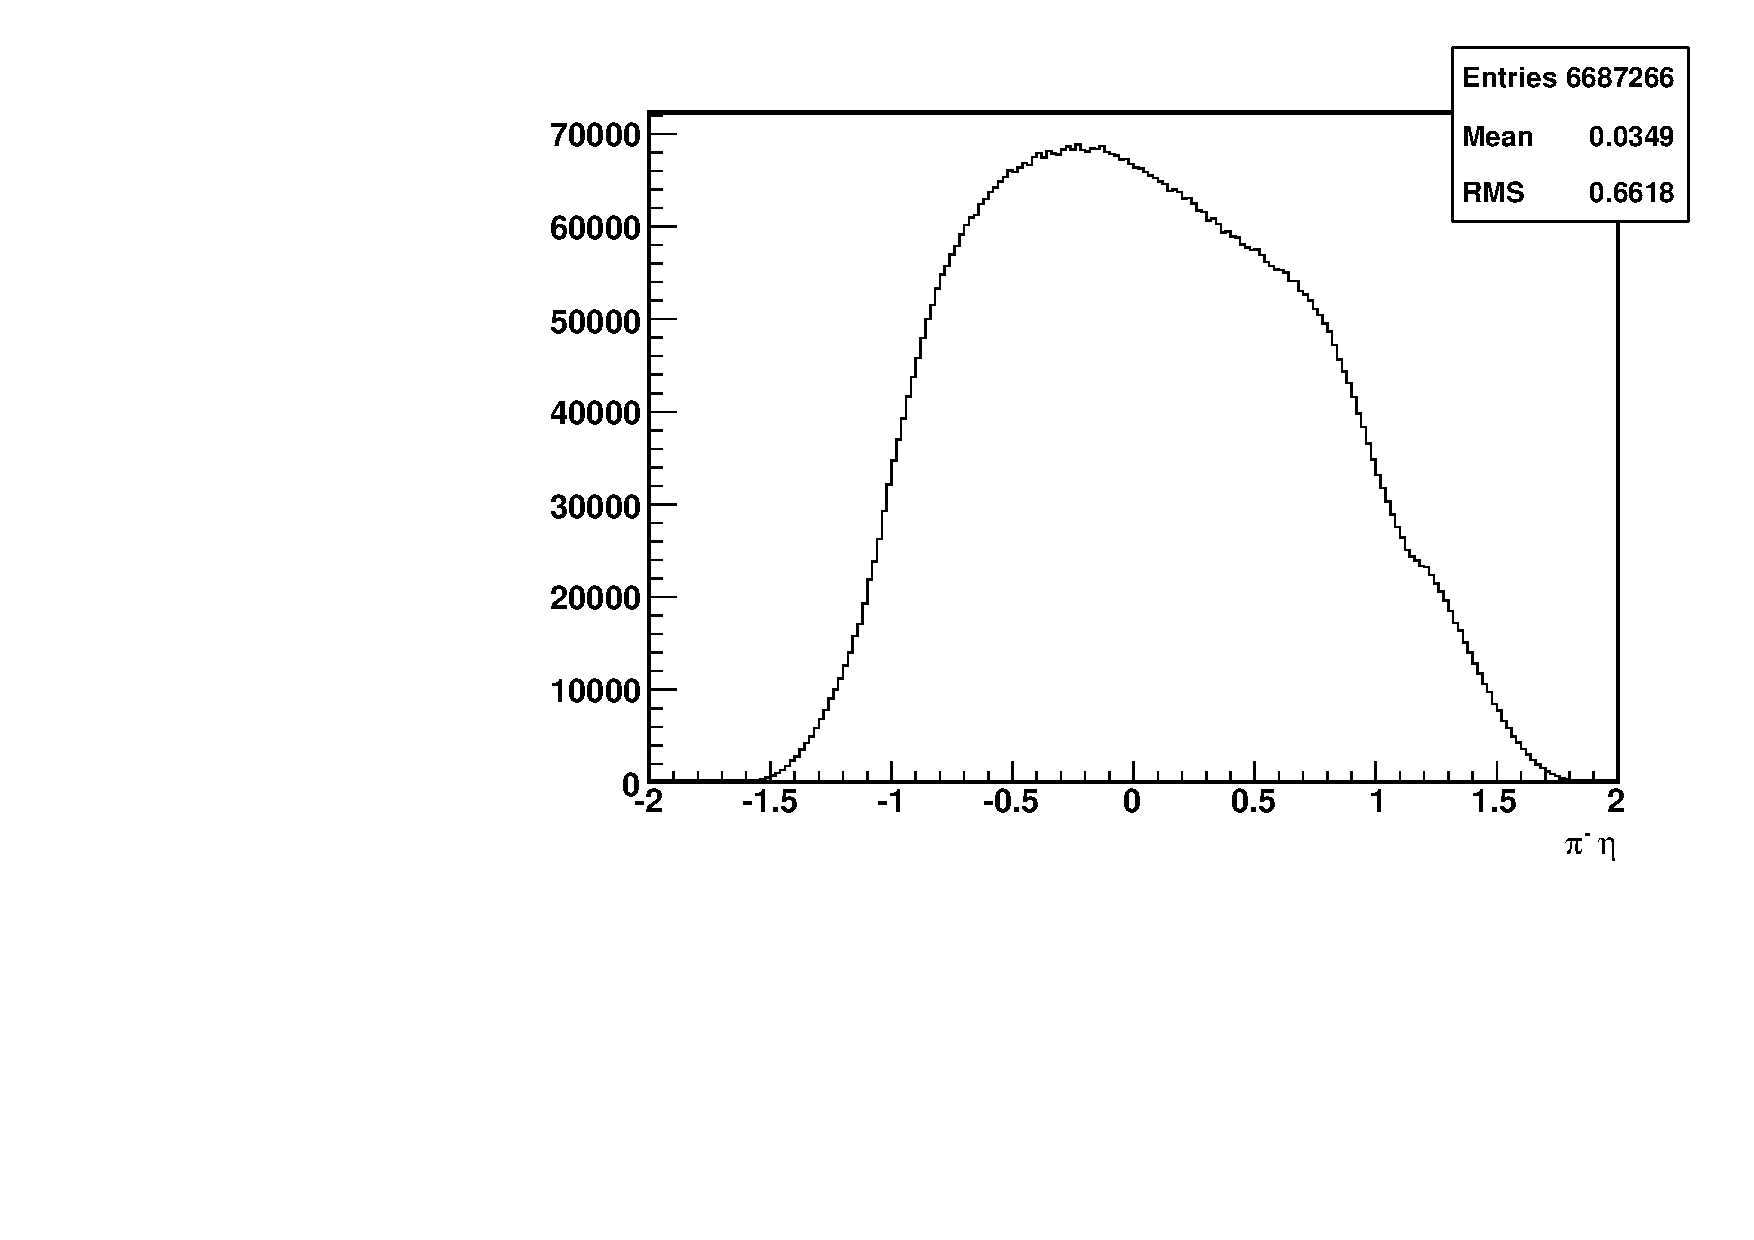
\includegraphics[width = .8\textwidth]{hNegEta}
\caption[$\eta$ distribution of $\pi^-$]{}
\label{fig:}
\end{center}
\end{figure}

\begin{figure}
\begin{center}
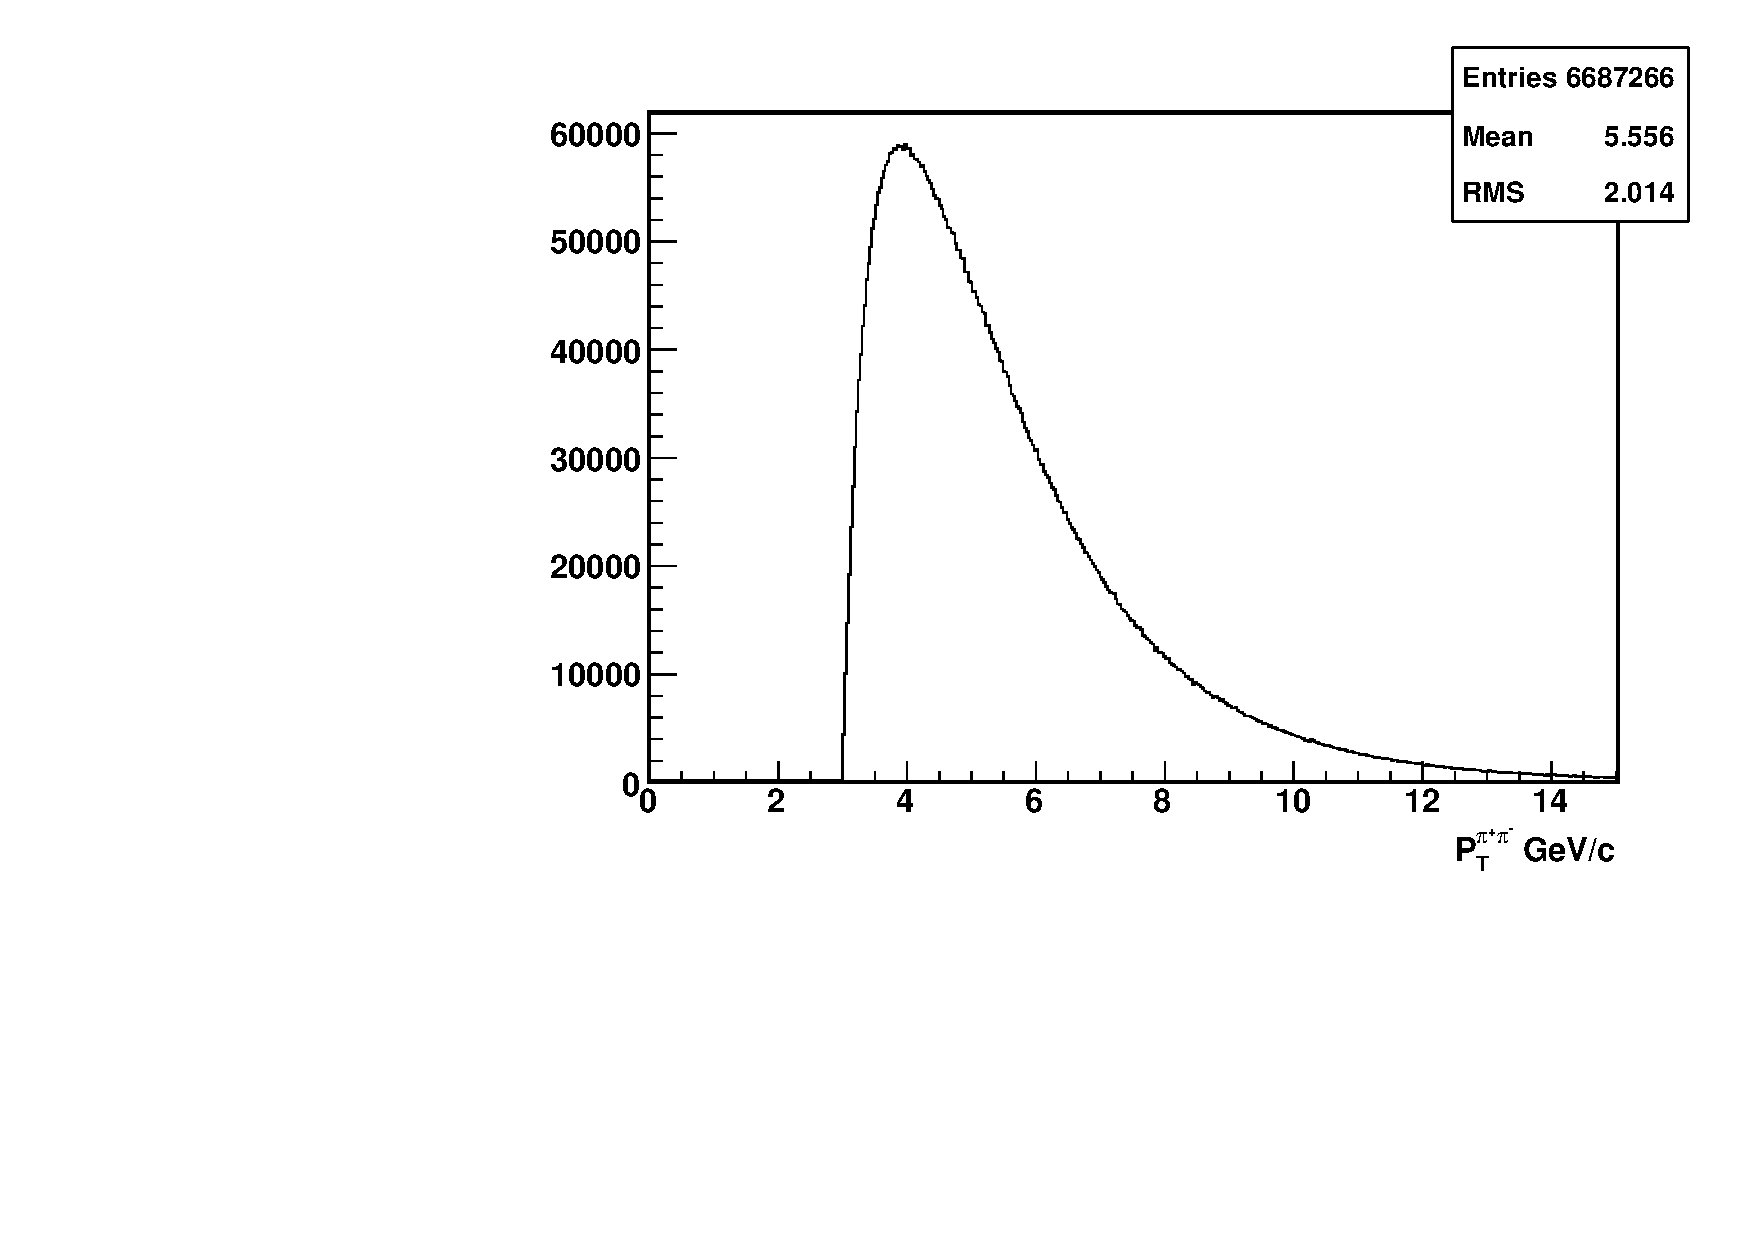
\includegraphics[width = .8\textwidth]{hPtPair}
\caption[$P_{T}$ distribution of \pair pair]{}
\label{fig:}
\end{center}
\end{figure}

\begin{figure}
\begin{center}
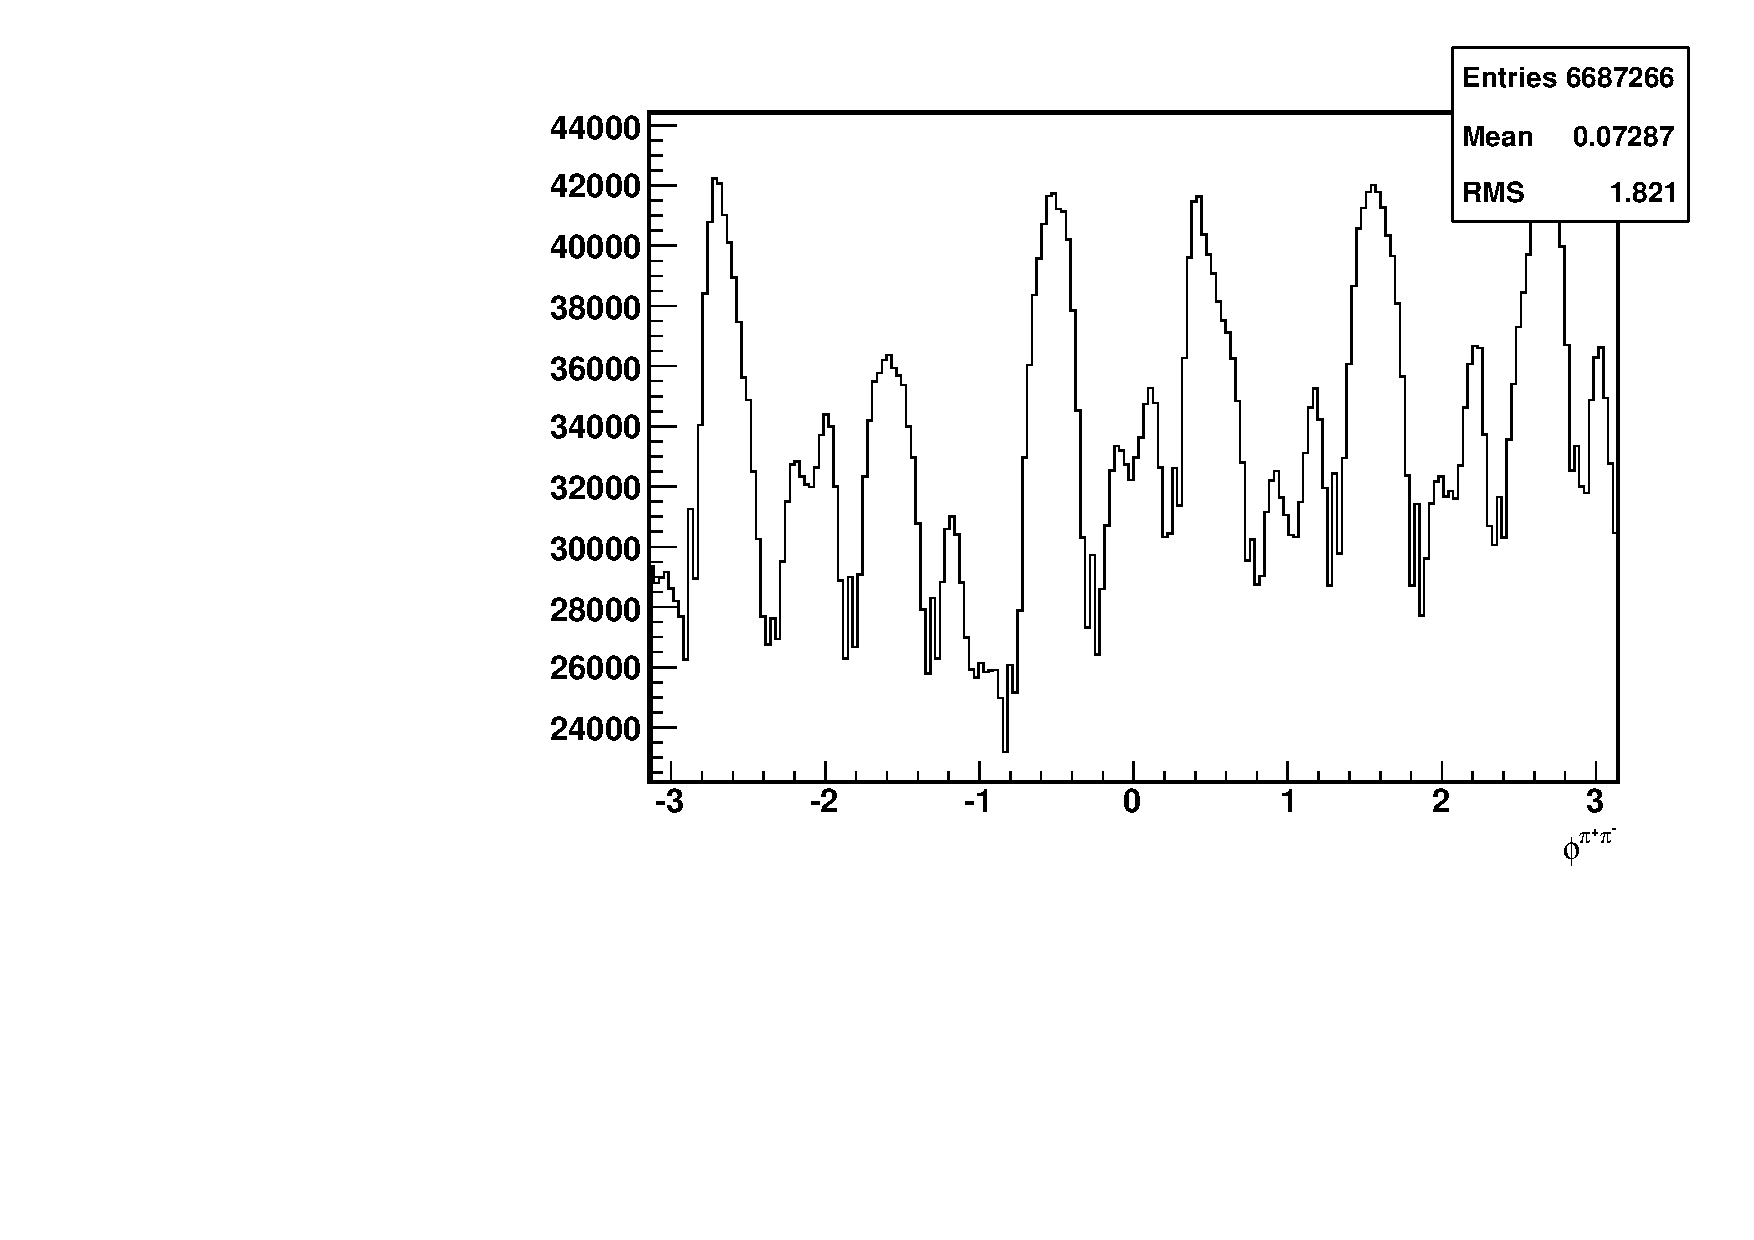
\includegraphics[width = .8\textwidth]{hPhiPair}
\caption[$\phi$ distribution of \pair pair]{}
\label{fig:}
\end{center}
\end{figure}

\begin{figure}
\begin{center}
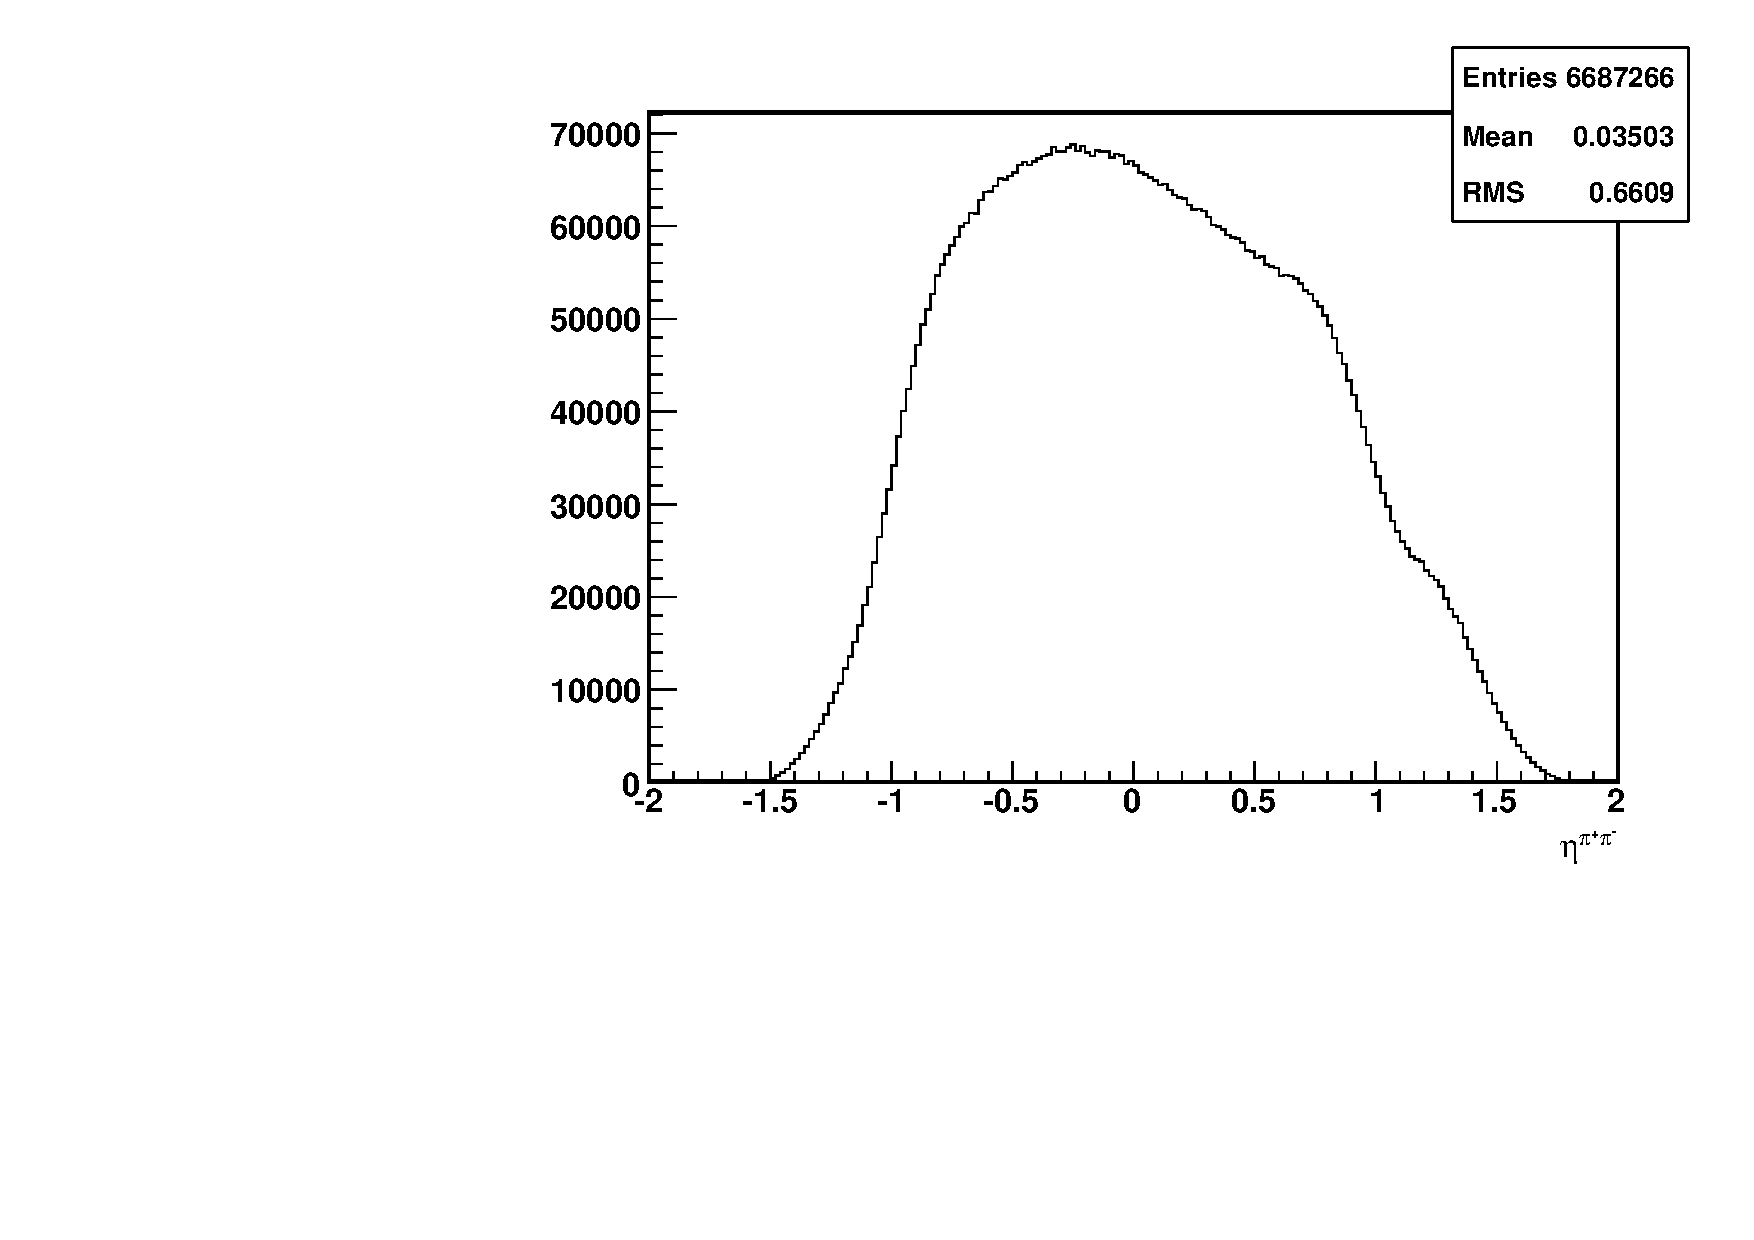
\includegraphics[width = .8\textwidth]{hEtaPair}
\caption[$\eta$ distribution of \pair pair]{}
\label{fig:}
\end{center}
\end{figure}


\begin{figure}
\begin{center}
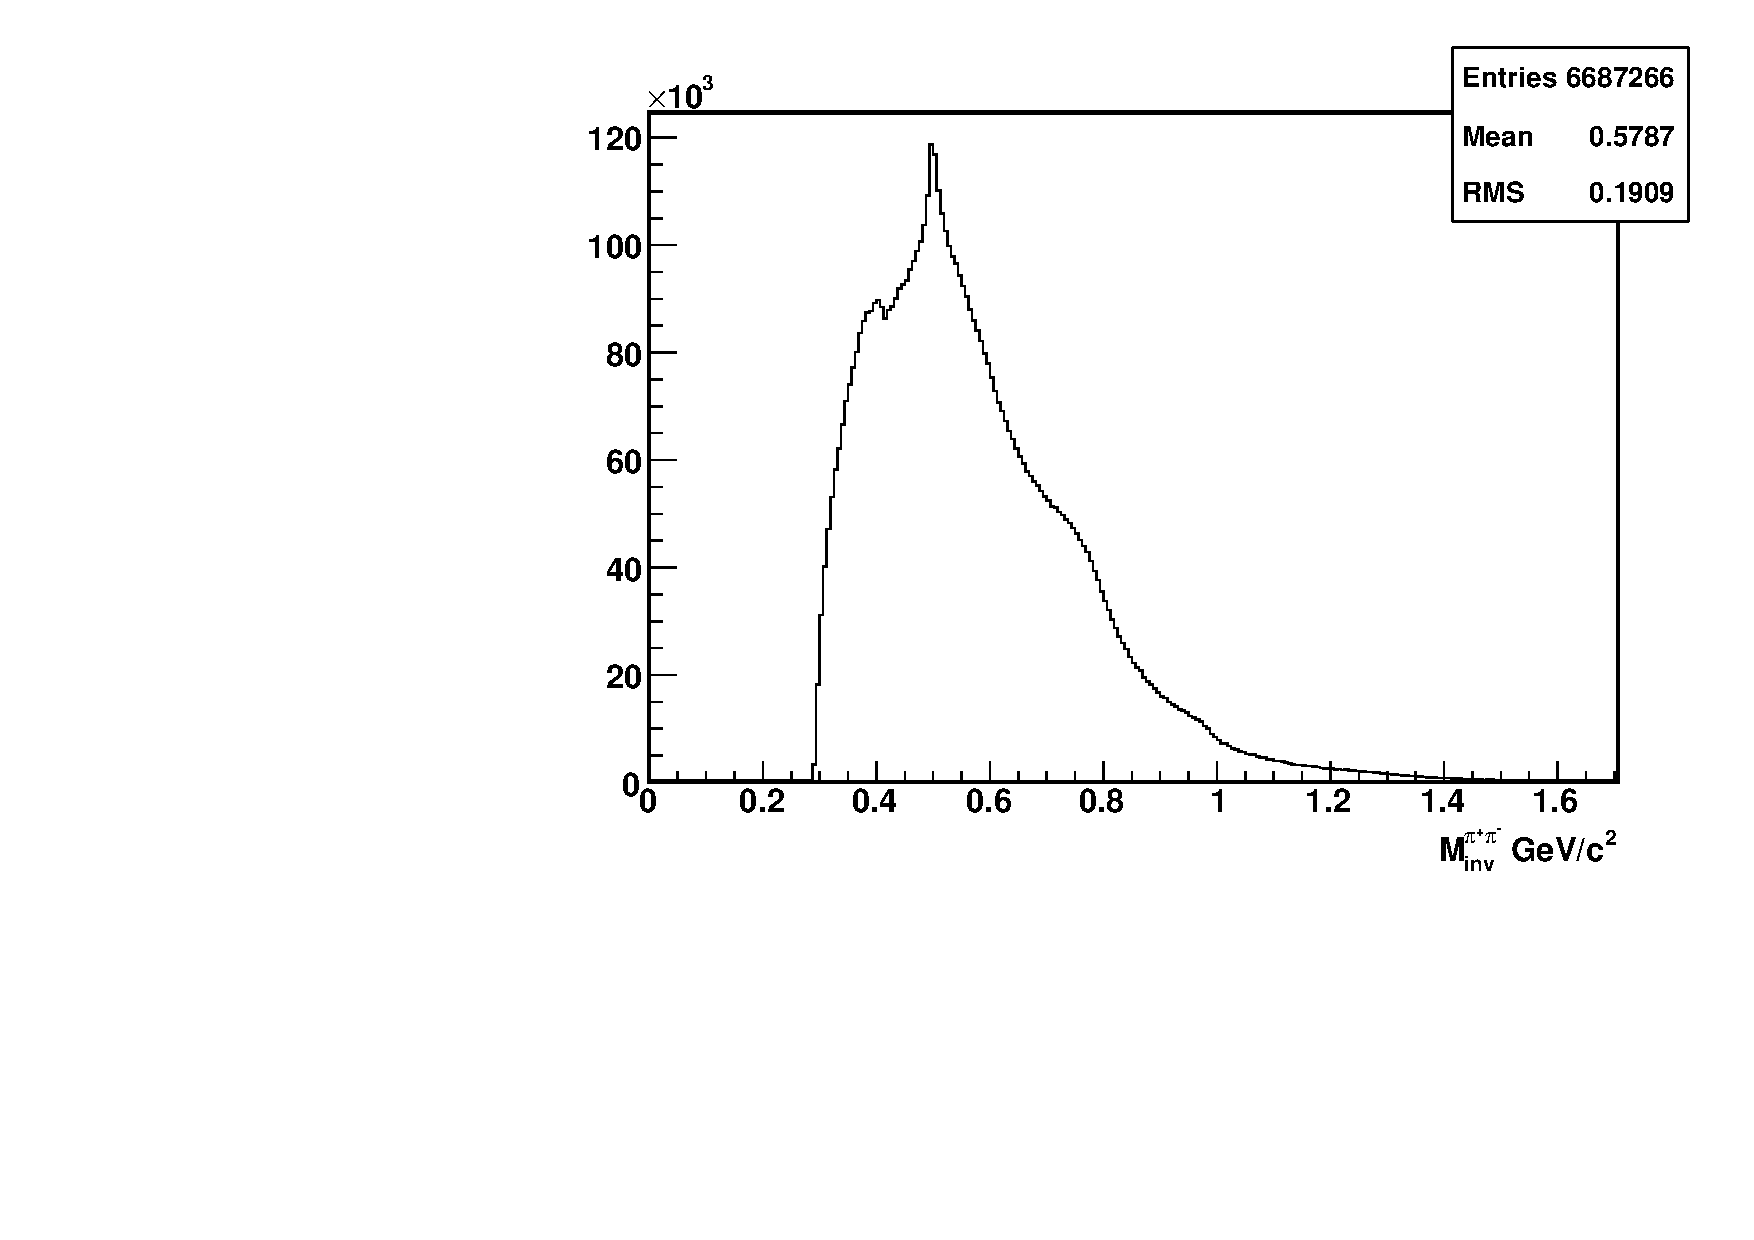
\includegraphics[width = .8\textwidth]{hInvarM}
\caption[Invariant mass distribution of \pair pair]{}
\label{fig:}
\end{center}
\end{figure}

\begin{figure}
\begin{center}
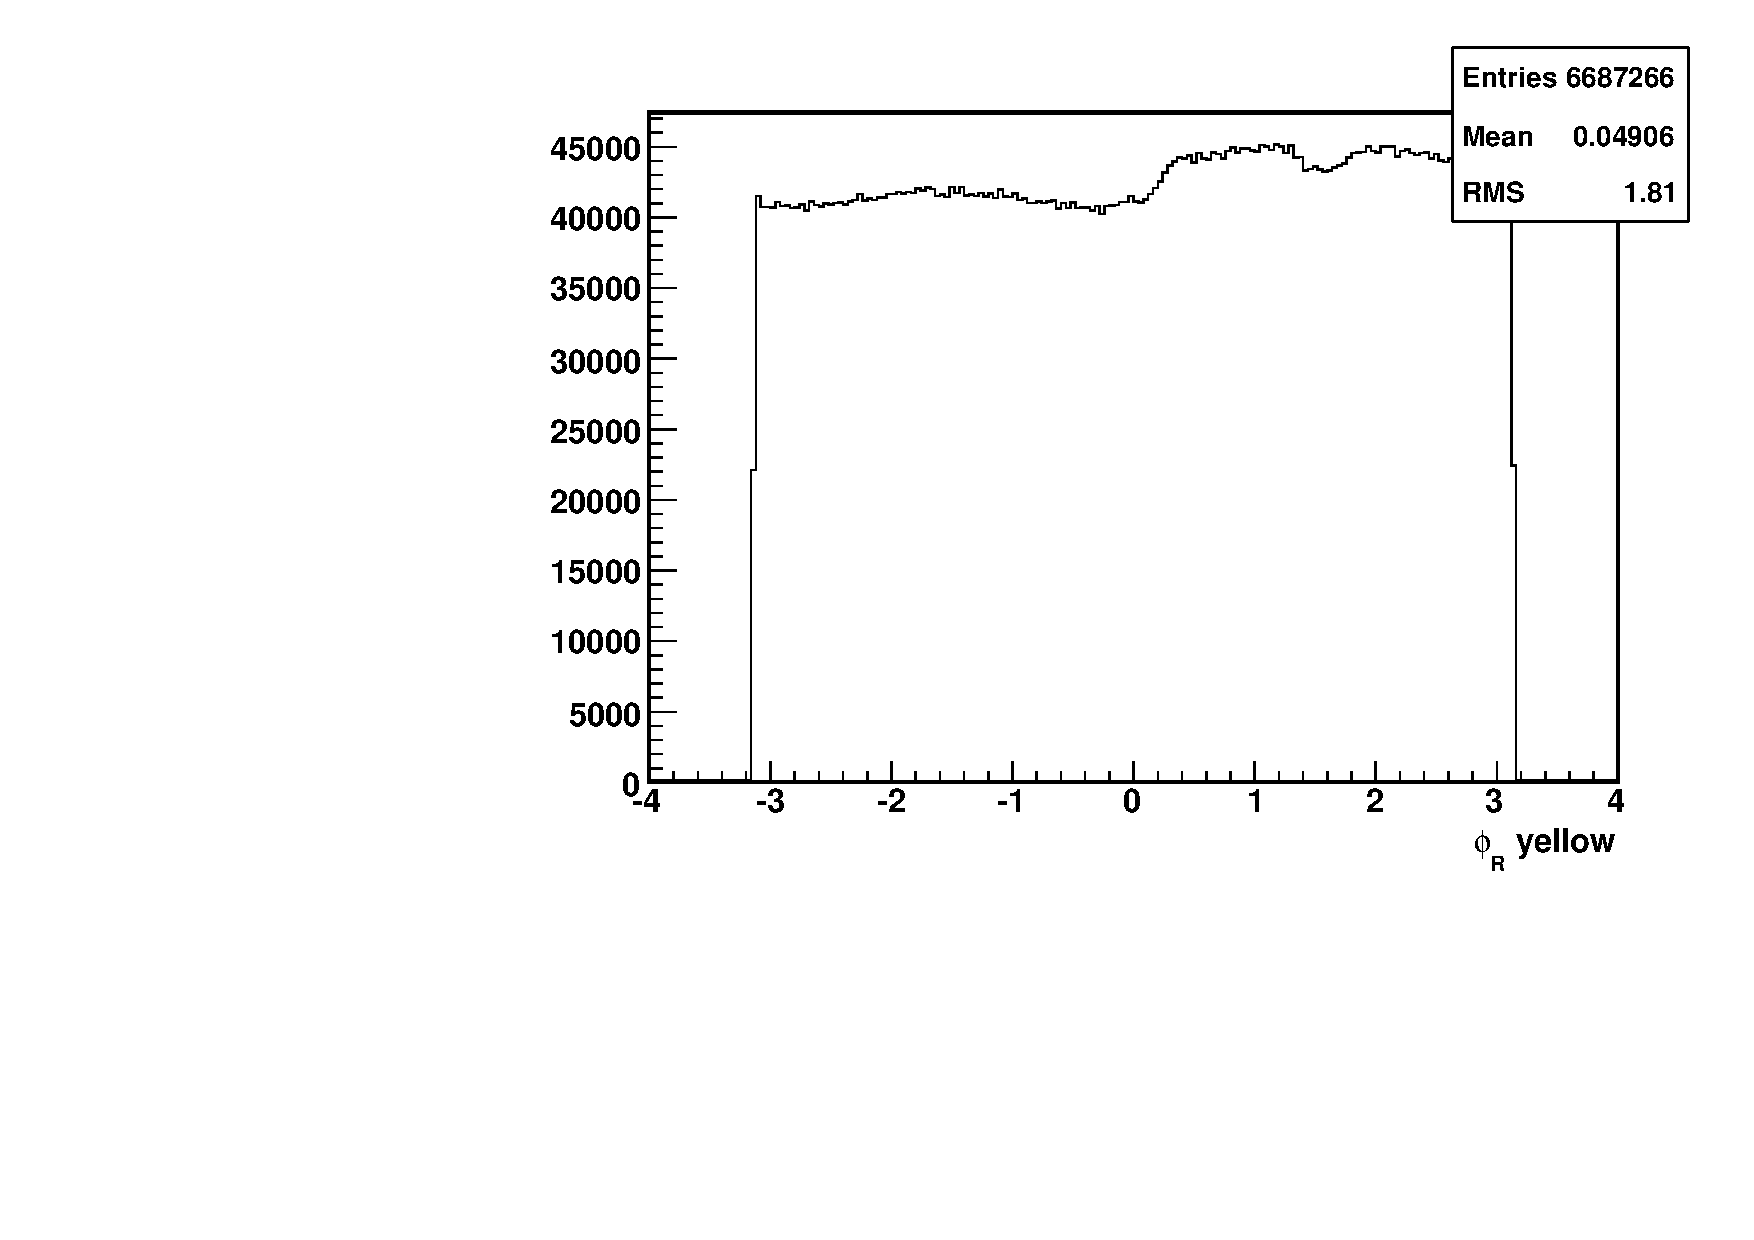
\includegraphics[width = .8\textwidth]{hPhiRy}
\caption[$\phir$ distribution of \pair pair with reference to the yellow beam polarization]{}
\label{fig:}
\end{center}
\end{figure}


\begin{figure}
\begin{center}
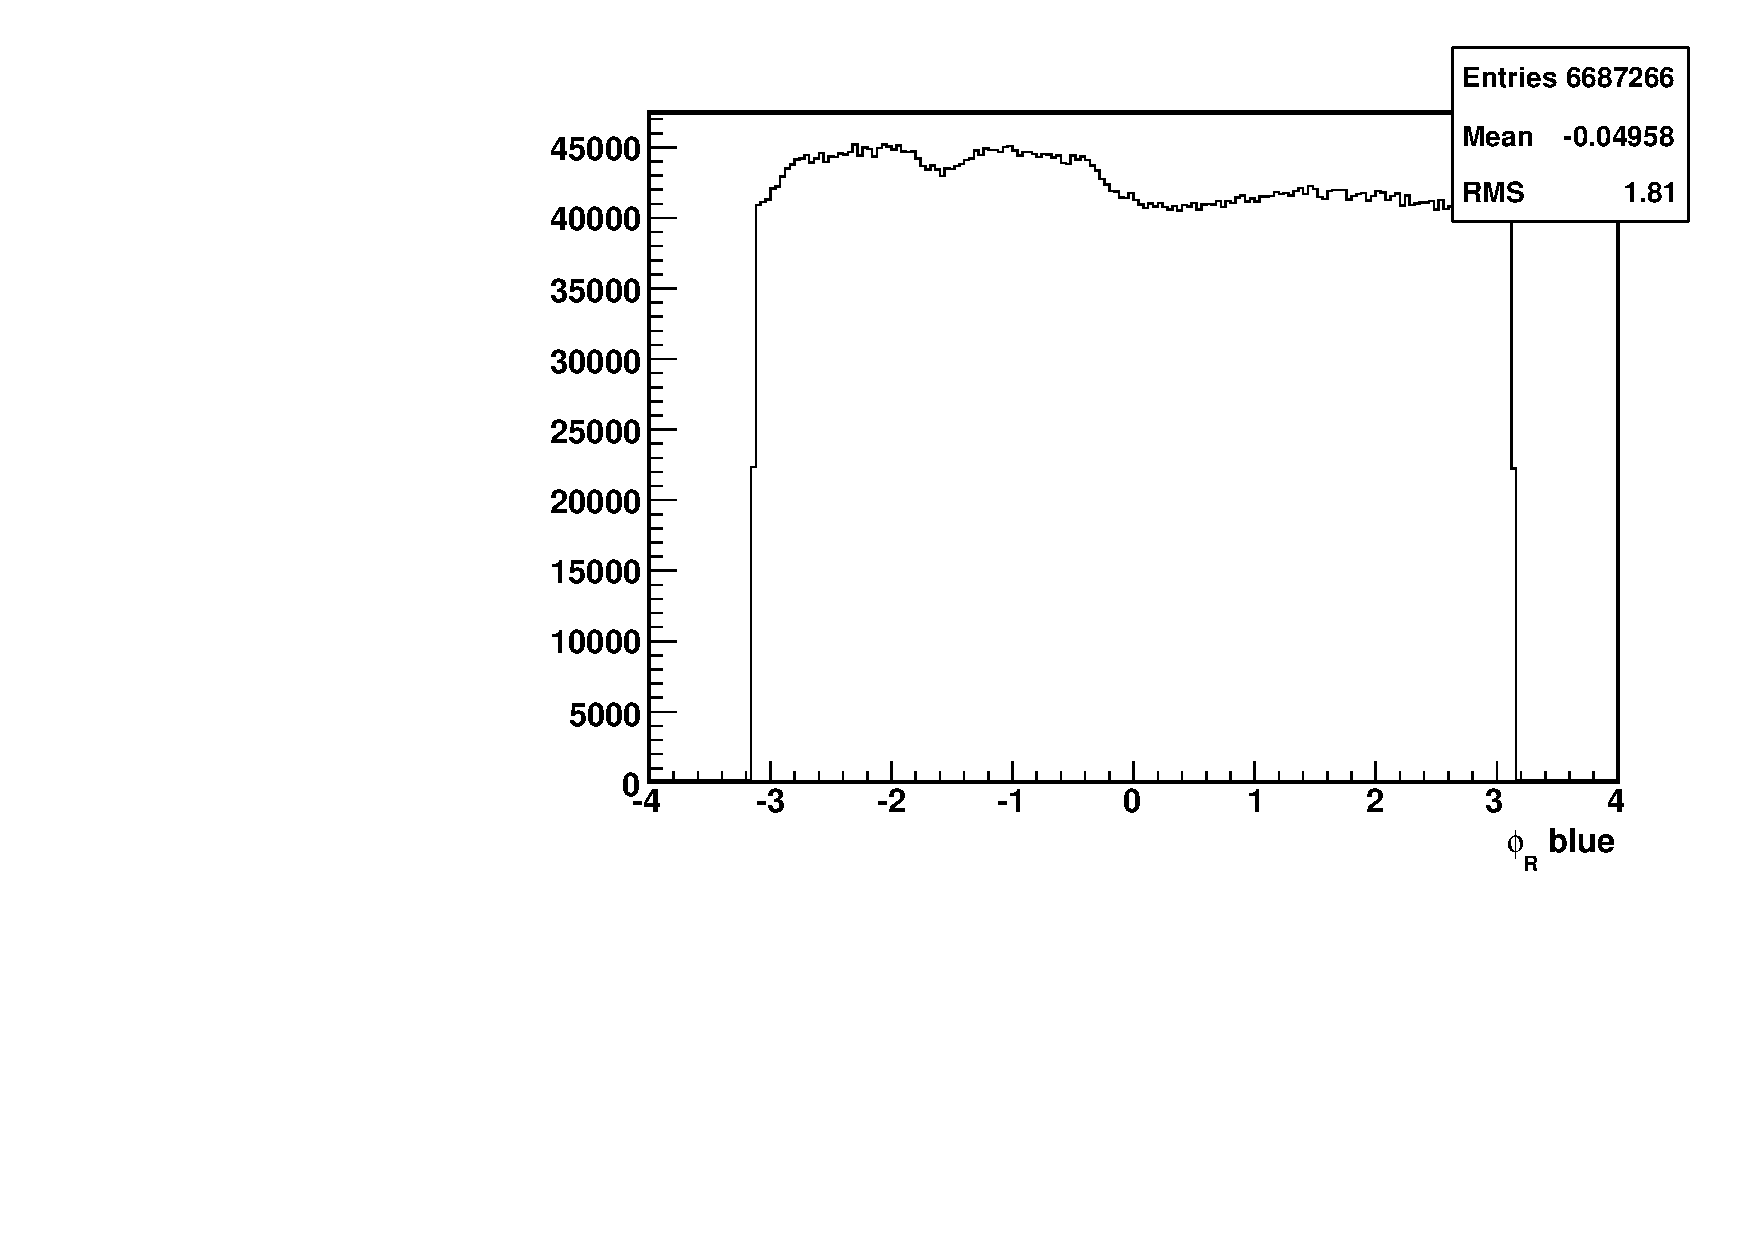
\includegraphics[width = .8\textwidth]{hPhiRb}
\caption[$\phir$ distribution of \pair pair with reference to the blue beam polarization]{}
\label{fig:}
\end{center}
\end{figure}


\begin{figure}
\begin{center}
\includegraphics[width = .8\textwidth]{hPhiSy}
\caption[$\phis$ distribution of \pair pair with reference to the yellow beam polarization]{}
\label{fig:}
\end{center}
\end{figure}


\begin{figure}
\begin{center}
\includegraphics[width = .8\textwidth]{hPhiSb}
\caption[$\phis$ distribution of \pair pair with reference to the blue beam polarization]{}
\label{fig:}
\end{center}
\end{figure}


\begin{figure}
\begin{center}
\includegraphics[width = .8\textwidth]{hPhiSRy}
\caption[$\phirs$ distribution of \pair pair with reference to the yellow beam polarization]{}
\label{fig:}
\end{center}
\end{figure}


\begin{figure}
\begin{center}
\includegraphics[width = .8\textwidth]{hPhiSRb}
\caption[$\phirs$ distribution of \pair pair with reference to the blue beam polarization]{}
\label{fig:}
\end{center}
\end{figure}


\begin{figure}
\begin{center}
\includegraphics[width = .8\textwidth]{hTheta}
\caption[$\theta$ distribution of \pair pair]{}
\label{fig:}
\end{center}
\end{figure}


\begin{figure}
\begin{center}
\includegraphics[width = .8\textwidth]{hCosTheta}
\caption[$\cos\theta$ distribution of \pair pair]{}
\label{fig:cosTheta}
\end{center}
\end{figure}


\begin{figure}
\begin{center}
\includegraphics[width = 1\textwidth]{invMassSameVsOpp4}
\caption[Invariant mass of opposite and same sign pion pairs]{Invariant mass of \pair pairs (black) and $\pi^+\pi^+$,$\pi^-\pi^-$ pairs (red). The histograms are normalized to a total area of 1 unit to account for differing numbers of opposite and same sign pairs found.}
\label{fig:invMSO}
\end{center}
\end{figure}

\begin{figure}
\begin{center}
\includegraphics[width = 1\textwidth]{diffInvMassSameOpp2}
\caption[Difference in the invariant mass of opposite and same sign pion pairs]{Difference in Invariant mass of \pair pairs and $\pi^+\pi^+$,$\pi^-\pi^-$ pairs}
\label{fig:dInvMSO}
\end{center}
\end{figure}



\section{Determining the angles}

The angles $\phir$ and $\phis$ seen in figure \ref{fig:angleDeff} are defined in equation \ref{eq:angles} according to \cite{bacchettaRedici2}. When calculating the angles, the spin vector of the proton is always taken to be up. In this case the angles $\phir$ and $\phis$ represent the spacial orientation of the pion pair.  

\begin{equation}
\label{eq:angles}
\begin{aligned}[c]
\cos\phi_S &= \frac{(\bm{\hat{P}}_b \times \bm{P}_h)}{|\bm{\hat{P}}_b \times \bm{P}_h|} \cdot \frac{(\bm{\hat{P}}_b \times \bm{S}_b)}{|\bm{\hat{P}}_b \times \bm{S}_b|} \\
\cos\phi_R &= \frac{(\bm{\hat{P}}_h \times \bm{P}_a)}{|\bm{\hat{P}}_h \times \bm{P}_a|} \cdot \frac{(\bm{\hat{P}}_h \times \bm{R})}{|\bm{\hat{P}}_h \times \bm{R}|} \\
\end{aligned}
\qquad
\begin{aligned}[c]
\sin\phi_S &= \frac{(\bm{P}_h \times \bm{S}_b) \cdot \bm{\hat{P}}_b}{|\bm{\hat{P}}_b \times \bm{P}_h| |\bm{\hat{P}}_b \times \bm{S}_b|} \\
\sin\phi_R &= \frac{(\bm{P}_a \times \bm{R}) \cdot \bm{\hat{P}}_h}{|\bm{\hat{P}}_h \times \bm{P}_a| |\bm{\hat{P}}_h \times \bm{R}|} 
\end{aligned}
\end{equation}\\




\FloatBarrier
\section{Calculating The Asymmetry}




\subsubsection{Luminosity Method}

To calculate the asymmetry using the luminosity method, 

\begin{equation}
A_{UT}P\sin\left(\phi_{RS}\right) = \frac{\frac{N^\uparrow}{L^\uparrow} - \frac{N^\downarrow}{L^\downarrow}} {\frac{N^\uparrow}{L^\uparrow} + \frac{N^\downarrow}{L^\downarrow}}
\end{equation}

$\phi_{RS}$ can take values from $-\pi$ to $\pi$



\subsubsection{Cross Ratio Method}

A more clever way of constructing the asymmetry is with the cross ratio method. I break the angle $\phi_{RS}$ up into 32 bins. I then count the number of pion pairs in that $\phi_{RS}$ bin when the polarization is up $N^\uparrow_{\phi_{RS}}$. 

\begin{equation}
\label{eq:nup}
N^\uparrow_{\phi_{RS}} = L^\uparrow I_{\phi_{RS}}(\theta)\left[1+A_{UT}P\sin(\phi_{RS})\right]
\end{equation}
%
In the above equation $I_{\phi_{RS}}(\theta)$ is the unpolarized cross section into the designated $\phi_{RS}$ bin and polar angle $\theta$, $L^\uparrow$ is the luminosity when the beam is in the spin up polarization, and P is the polarization percentage of the beam. The asymmetry causes an enhancement in the number of pion pairs we see. Next we look at the number of pairs we see in the same $\phi_{RS}$ bin when the spin is down.

\begin{equation}
\label{eq:ndwn}
N^\downarrow_{\phi_{RS}} = L^\downarrow I_{\phi_{RS}}(\theta)\left[1-A_{UT}P\sin(\phi_{RS})\right]
\end{equation}
%
This time the spin in down so the plus sign in equation \ref{eq:nup} becomes a negative. This tells us that the number of pairs we see from a spin down polarization is decreased. 
Next we want to look at what happens when we change the $\phi_{RS}$ bin by $\pi$. Still counting when the polarization is spin down we see that:

\begin{equation}
N^\downarrow_{\phi_{RS}+\pi} = L^\downarrow I_{\phi_{RS}+\pi}(\theta)\left[1+A_{UT}P\sin(\phi_{RS})\right]
\end{equation}
%
Since $\sin(x+\pi) = -\sin(x)$, the negative sign from equation \ref{eq:ndwn} has flipped again. Finally if we look at bin $\phi_{RS} + \pi$, with a spin up polarization we see the sign flip one more time. 

\begin{equation}
N^\uparrow_{\phi_{RS}+\pi} = L^\uparrow I_{\phi_{RS}+\pi}(\theta)\left[1-A_{UT}P\sin(\phi_{RS})\right]
\end{equation}
%
We then define "left" and "right"\footnote{Called left and right because the cross ratio was first used in experiments measuring asymmetries in particle production detected in two different detectors. One of these detectors was situated to the left of the incident beam and the other to the right.} as 
\begin{equation}
\mathcal{L} = \sqrt{N^\uparrow_{\phi_{RS}}N^\downarrow_{\phi_{RS}+\pi}}  = \sqrt{L^\uparrow L^\downarrow I_{\phi_{RS}} I_{\phi_{RS}+\pi}} \left[ 1+A_{UT}P\sin(\phi_{RS})\right]
\end{equation}

\begin{equation}
\mathcal{R} = \sqrt{N^\downarrow_{\phi_{RS}}N^\uparrow_{\phi_{RS}+\pi}} = \sqrt{L^\uparrow L^\downarrow I_{\phi_{RS}} I_{\phi_{RS}+\pi}} \left[ 1-A_{UT}P\sin(\phi_{RS})\right]
\end{equation}
%
The combination $\frac{\mathcal{L} - \mathcal{R}}{\mathcal{L} + \mathcal{R}}$  gives an expression independent of luminosities. 

\begin{equation}
\label{eq:crossRatio}
\frac{\mathcal{L} - \mathcal{R}}{\mathcal{L} +\mathcal{R}} = \frac{\sqrt{N^\uparrow_{\phi_{RS}}N^\downarrow_{\phi_{RS}+\pi}} - \sqrt{N^\downarrow_{\phi_{RS}}N^\uparrow_{\phi_{RS}+\pi}}}{\sqrt{N^\uparrow_{\phi_{RS}}N^\downarrow_{\phi_{RS}+\pi}} + \sqrt{N^\downarrow_{\phi_{RS}}N^\uparrow_{\phi_{RS}+\pi}}} = A_{UT}P\sin(\phi_{RS})
\end{equation}\\
%
or in other words
\begin{equation}
\label{eq:crossRatio2}
A_{UT}\sin\left(\phirs\right) = \frac{1}{P}\frac{\sqrt{N^\uparrow_{\phi_{RS}}N^\downarrow_{\phi_{RS}+\pi}} - \sqrt{N^\downarrow_{\phi_{RS}}N^\uparrow_{\phi_{RS}+\pi}}}{\sqrt{N^\uparrow_{\phi_{RS}}N^\downarrow_{\phi_{RS}+\pi}} + \sqrt{N^\downarrow_{\phi_{RS}}N^\uparrow_{\phi_{RS}+\pi}}}
\end{equation}\\



Equation \ref{eq:crossRatio2} is called the cross ratio and is what I will use throughout my analysis. As stated, this form of the asymmetry is nice because luminosity and detector effects are canceled. This helps us for multiple reasons. The uncertainty in luminosity is difficult to pin down as the luminosity can fluctuate. So not having to take this into account is good. Also detector irregularities causing more pairs to be found near a "hot tower" are canceled.

probably move below to next section.

One thing to note is that only 16 of my original 32 $\phi_{RS}$ bins are unique because I have double counted. This is because I use the same number for $N^\uparrow_{\phi_{RS}}$ for $\phi_{RS}$ bin 1 and for $N^\uparrow_{\phi_{RS}+\pi}$ for $\phi_{RS}$ bin 9. The unique range of $\phi_{RS}$ I choose to use is $-\pi/2$ to $\pi/2$

In order to extract the asymmetry, a histogram of $\frac{1}{P}\frac{\mathcal{L} - \mathcal{R}}{\mathcal{L} + \mathcal{R}}$ is constructed. This is then fit with a sine function ($A\sin(\phirs)$ ), and the resulting amplitude of the fit is taken as $A_{UT}$. This is done for different kinematic bins. An example of this fitting is shown in figure \ref{fig:sinFit}. 

The errors for $N^\uparrow$ and $N^\downarrow$ in each $\phirs$ bin is taken as the poisson error of $\sqrt{N^\uparrow}$ or $\sqrt{N^\uparrow}$ for that bin. By propagating this through, we find the relevant bin error:

\begin{align}
\delta\left(\frac{1}{P}\frac{\mathcal{L} - \mathcal{R}}{\mathcal{L} + \mathcal{R}}\right)_{\phirs} & = \frac{1}{P^2 \left(\sqrt{\nup_{\phirs} \ndw_{\phirs+\pi}} + \sqrt{\ndw_{\phirs}\nup_{\phirs + \pi}}\right)^2} \nonumber \\
& \times \sqrt{P^2\left[   \nup_{\phirs+\pi} \ndw_{\phirs} \left( \ndw_{\phirs+\pi} + \nup_{\phirs}\right) +  \ndw_{\phirs+\pi} \nup_{\phirs} \left( \nup_{\phirs+\pi} + \ndw_{\phirs}\right) \right]}
\end{align}
%
A smaller correction to the error due to the error on the polarization measurement is left out because it is significantly smaller than the term shown above.



\begin{figure}
\begin{center}
\includegraphics[width = 1\textwidth]{sinFit3}
\caption[Sinusoid modulation of \pair pair produciton and fit for 9 $\ptpair$ bins]{Example of the sine fitting. Here different pair transverse momentum ranges are fit with a sine. as the transverse momentum increases, the amplitude of the fit, and thus the asymmetry $A_{UT}$, increases.}
\label{fig:sinFit}
\end{center}
\end{figure}

\begin{sidewaysfigure}
\begin{center}
\includegraphics[width = 1\textwidth]{sinFit3}
\caption[Sinusoid modulation of \pair pair produciton and fit for 9 $\ptpair$ bins]{Example of the sine fitting. Here different pair transverse momentum ranges are fit with a sine. as the transverse momentum increases, the amplitude of the fit, and thus the asymmetry $A_{UT}$, increases.}
\label{fig:sinFit}
\end{center}
\end{sidewaysfigure}



\subsubsection{Code}

Ideally the polarization of the beam will be constant throughout the entire data set, however this is not possible. Because of this, the way the asymmetry is calculated in the analysis code is slightly different. The following section will be a detailed explanation of how exactly it is calculated. 


For a concrete example, lets say we want to calculate the asymmetry for different pair transverse momenta. First the transverse momentum is broken up into different bins. For each of these bins, a set of several histograms are created. Two of these histograms are responsible for storing the number of pairs from spin up and from spin down. The x-axis of these histograms, which represent $\phirs$, is broken up into 32 bins and range from $-\pi$ to $\pi$. For every pair, these histograms are incremented by one at the corresponding value of $\phirs$. In this manner they hold the number of pairs from spin up and down at every value of $\phirs$. The other two histograms are responsible for storing the transverse momentum of each pair and eventually to store the values to be fit for the asymmetry respectively.

Not yet mentioned is the beam polarization. To handle this, four more histograms are created for each of the 32 $\phirs$ bins. These histograms store the beam polarization of pairs from spin up and down events, as well as the error of the beam polarization squared from spin up and spin down events. The latter will be used when calculating errors. The analysis code loops through the data set and fills the correct histograms with the correct information. Once this is completed the calculation of the asymmetry is performed. 

Because the polarization can differ between spin up and down pairs as well as between $\phirs$ bins, I alter how the polarization is used in the calculation compared to equation \ref{eq:crossRatio2}. Instead of having one value for the polarization, I use several values for the polarization, one for each spin state and $\phirs$ bin.    
 

\begin{equation}
\label{eq:crossRatioCode}
A_{UT}\sin(\phi_{RS} ) = \frac{\sqrt{\frac{N^\uparrow_{\phi_{RS}}}{\left<p^\uparrow_{\phirs}\right>} \frac{N^\downarrow_{\phi_{RS}+\pi}}{\left<p^\downarrow_{\phirs+\pi}\right>}} - \sqrt{\frac{N^\uparrow_{\phi_{RS}+\pi}}{\left<p^\uparrow_{\phirs+\pi}\right>} \frac{N^\downarrow_{\phi_{RS}}}{\left<p^\downarrow_{\phirs}\right>}}}       {\sqrt{N^\uparrow_{\phi_{RS}} N^\downarrow_{\phi_{RS}+\pi}} + \sqrt{N^\uparrow_{\phi_{RS}+\pi} N^\downarrow_{\phi_{RS}}}}
\end{equation}\\
%
Where $\left<p^\uparrow_{\phirs}\right>, \left<p^\downarrow_{\phirs+\pi}\right>, \left<p^\uparrow_{\phirs+\pi}\right>, \textnormal{ and } \left<p^\downarrow_{\phirs}\right>$ are the average beam polarizations in pairs from spin up, down events and at angle $\phirs$, $\phirs + \pi$. Therefore the number of pairs from each spin state and angle are weighted by their own separate average polarization.   

The histogram responsible for storing the values to be fit is now used. The x-axis of this histogram is also separated into 32 $\phirs$ bins and ranges from $-\pi$ to $\pi$. For each $\phirs$ bin the left hand side of equation \ref{eq:crossRatioCode} is calculated and used to set the value of the corresponding $\phirs$ bin in the to fit histogram.

The bin errors seen in figure \ref{fig:sinFit} are also set by hand but are a little more intricate. 

\begin{equation}
\label{eq:epsilon}
\textnormal{Let } \mathcal{E} = \frac{\sqrt{\frac{N^\uparrow_{\phi_{RS}}}{\left<p^\uparrow_{\phirs}\right>} \frac{N^\downarrow_{\phi_{RS}+\pi}}{\left<p^\downarrow_{\phirs+\pi}\right>}} - \sqrt{\frac{N^\uparrow_{\phi_{RS}+\pi}}{\left<p^\uparrow_{\phirs+\pi}\right>} \frac{N^\downarrow_{\phi_{RS}}}{\left<p^\downarrow_{\phirs}\right>}}}       {\sqrt{N^\uparrow_{\phi_{RS}} N^\downarrow_{\phi_{RS}+\pi}} + \sqrt{N^\uparrow_{\phi_{RS}+\pi} N^\downarrow_{\phi_{RS}}}}
\end{equation}\\

The error on $\mathcal{E}$ is defined as $\delta \mathcal{E} = \sqrt{E^2_{stat} + E^2_{pol}}$. Where $E^2_{stat}$ is the statistical error and $E^2_{pol}$ is the error from the polarization uncertainty. Let's look at these two individually starting with the statistical error term.

To make our lives easier lets introduce two new variables, $a = \sqrt{N^\uparrow_{\phi_{RS}}N^\downarrow_{\phi_{RS}+\pi}}$ and $b = \sqrt{N^\uparrow_{\phi_{RS}+\pi}N^\downarrow_{\phi_{RS}}}$

Rewriting equation \ref{eq:epsilon} with these new variables, gives

\begin{equation}
\label{eq:epsilonAB}
\mathcal{E} = \frac{\frac{a}{\sqrt{\left<p^\uparrow_{\phirs}\right>\left<p^\downarrow_{\phirs+\pi}\right>}}  - \frac{b}{\sqrt{\left<p^\uparrow_{\phirs+\pi}\right>\left<p^\downarrow_{\phirs}\right>}}} {a+b}
\end{equation}\\
%
With this notation, the statistical error becomes

\begin{equation}
\label{eq:Estat}
E_{stat}^2 = \left(\frac{\partial \mathcal{E}}{\partial a}\right)^2 {\delta a}^2 + \left(\frac{\partial \mathcal{E}}{\partial b}\right)^2 {\delta b}^2
\end{equation}\\
%
The errors on a and b are similarly calculated. 


\begin{align}
{\delta a}^2 &= \left(\frac{\partial a}{\partial N^\uparrow_{\phirs}}\right)^2 \left(\delta N^\uparrow_{\phirs}\right)^2 + \left(\frac{\partial a}{\partial N^\downarrow_{\phirs+\pi}}\right)^2 \left(\delta N^\downarrow_{\phirs+\pi}\right)^2 \\
{\delta b}^2 &= \left(\frac{\partial b}{\partial N^\uparrow_{\phirs+\pi}}\right)^2 \left(\delta N^\uparrow_{\phirs+\pi}\right)^2 + \left(\frac{\partial b}{\partial N^\downarrow_{\phirs}}\right)^2 \left(\delta N^\downarrow_{\phirs}\right)^2 
\end{align}
%
Taking the errors on the number of pairs in a bin as $\delta N = \sqrt{N}$,

\begin{align}
{\delta a}^2 &= \frac{1}{4}\left(N^\uparrow_{\phirs}+ N^\downarrow_{\phirs+\pi}\right)\\
{\delta b}^2 &=  \frac{1}{4}\left(N^\uparrow_{\phirs+\pi}+ N^\downarrow_{\phirs}\right)
\end{align}
%
Putting everything together $E_{stat}$ becomes

\begin{align}
E_{stat}^2 = \frac{1}{4}\frac{1}{\left(a+b\right)^4} \left[\frac{1}{\sqrt{\left<p^\uparrow_{\phirs}\right>\left<p^\downarrow_{\phirs+\pi}\right>}}+\frac{1}{\sqrt{\left<p^\uparrow_{\phirs+\pi}\right>\left<p^\downarrow_{\phirs}\right>}}\right]^2 \\ \nonumber
\times \left[b^2\left(N^\uparrow_{\phirs} + N^\downarrow_{\phirs+\pi}\right) + a^2 \left(N^\uparrow_{\phirs+\pi} +  N^\downarrow_{\phirs} \right)\right]
\end{align}\\
%
Assuming all $N$s and polarizations are equal we see that the statistical error scales like $E_{stat}^2 \sim \frac{1}{p^2 N}$.

The error from the polarization uncertainty is a little bit trickier to tackle. Since each pair comes with it's own polarization uncertainty, I want to use all of them. To do this I have to change how I write $\mathcal{E}$. Namely I want to explicitly write out how each pair's polarization comes in instead of the average polarization. 

\begin{equation}
\label{eq:epsilonForPol}
\mathcal{E} = \frac{   \sqrt{\frac{{N^\uparrow_{\phirs}}^2 {N^\downarrow_{\phirs+\pi}}^2}{\sum\limits_{i=1}^{N^\uparrow_{\phirs}} p_i \sum\limits_{j=1}^{N^\downarrow_{\phirs+\pi}} p_j}} - \sqrt{\frac{{N^\downarrow_{\phirs}}^2 {N^\uparrow_{\phirs+\pi}}^2}{\sum\limits_{n=1}^{N^\downarrow_{\phirs}} p_n \sum\limits_{m=1}^{N^\uparrow_{\phirs+\pi}} p_m}}   }  {a+b}
\end{equation}\\
%
To obtain this form of $\mathcal{E}$ I have used, $\left<p_x\right> = \frac{1}{N_x}\sum\limits_{x=1}^{N_x} p_x$. 

By writing $\mathcal{E}$ as in equation \ref{eq:epsilonForPol}, it is clearer how the polarization uncertainty propagates to the error of $\mathcal{E}$.

\begin{equation}
\label{eq:Epol}
E_{pol}^2 = \sum\limits_{i=1}^{N^\uparrow_{\phirs}} \left(\frac{\partial\mathcal{E}}{\partial p_i}\right)^2 {\delta p_i}^2 + \sum\limits_{j=1}^{N^\downarrow_{\phirs+\pi}} \left(\frac{\partial\mathcal{E}}{\partial p_j}\right)^2  {\delta p_j}^2 + \sum\limits_{n=1}^{N^\downarrow_{\phirs}}\left(\frac{\partial\mathcal{E}}{\partial p_n}\right)^2  {\delta p_n}^2 +\sum\limits_{m=1}^{N^\uparrow_{\phirs+\pi}} \left(\frac{\partial\mathcal{E}}{\partial p_m}\right)^2  {\delta p_m}^2
\end{equation}\\
%
Computing the derivative $\frac{\partial\mathcal{E}}{\partial p_i}$ gives, 

\begin{equation}
\label{eq:singleDeriv}
\frac{\partial\mathcal{E}}{\partial p_i} = \frac{-1}{2(a+b)} \frac{a^2 \sum\limits_{j=1}^{N^\downarrow_{\phirs+\pi}}p_j}{\left(\sum\limits_{j=1}^{N^\downarrow_{\phirs+\pi}}p_i \sum\limits_{j=1}^{N^\downarrow_{\phirs+\pi}} p_j\right)^{3/2}}
\end{equation}\\
%
Using again the fact that $\left<p_x\right> = \frac{1}{N_x}\sum\limits_{x=1}^{N_x} p_x$, it follows that 
\begin{align}
\sum\limits_{i=1}^{N^\uparrow_{\phirs}} \left(\frac{\partial\mathcal{E}}{\partial p_i}\right)^2 {\delta p_i}^2 &= \sum\limits_{i=1}^{N^\uparrow_{\phirs}} \frac{a^4}{4(a+b)^2} \frac{{\delta p_i}^2}{{N^\uparrow_{\phirs}}^3\left<p^\uparrow_{\phirs}\right>^3N^\downarrow_{\phirs+\pi}\left<p^\downarrow_{\phirs+\pi}\right>} \\
& = \frac{1}{4} \frac{N^\downarrow_{\phirs+\pi}}{(a+b)^2} \frac{\left<{\delta p^\uparrow_{\phirs}}^2\right>}{\left<p^\uparrow_{\phirs}\right>^3\left<p^\downarrow_{\phirs+\pi}\right>}
\end{align}\\
%
Each term has a similar form. Putting them all together gives the error from the polarization uncertainty. 

\begin{align}
E_{pol}^2 = \frac{1}{4(a+b)^2} \Biggl[ N^\downarrow_{\phirs+\pi} \frac{\left<{\delta p^\uparrow_{\phirs}}^2\right>}{\left<p^\uparrow_{\phirs}\right>^3\left<p^\downarrow_{\phirs+\pi}\right>} + N^\uparrow_{\phirs} \frac{\left<{\delta p^\downarrow_{\phirs+\pi}}^2\right>}{\left<p^\downarrow_{\phirs+\pi}\right>^3\left<p^\uparrow_{\phirs}\right>} \\ \nonumber
+  N^\uparrow_{\phirs+\pi} \frac{\left<{\delta p^\downarrow_{\phirs}}^2\right>}{\left<p^\downarrow_{\phirs}\right>^3\left<p^\uparrow_{\phirs+\pi}\right>} + N^\downarrow_{\phirs} \frac{\left<{\delta p^\uparrow_{\phirs+\pi}}^2\right>}{\left<p^\uparrow_{\phirs+\pi}\right>^3\left<p^\downarrow_{\phirs}\right>} \Biggr]
\end{align}\\
%

To compare this error to the statistical error, lets check to see how it scales with the number of pairs in the same way we did before. It turns out $E_{pol}^2 \sim \frac{1}{p^2N} \frac{{\delta p}^2}{p^2}$. In other words the error due to the polarization uncertainty is smaller than the statistical error by a factor of $\frac{{\delta p}^2}{p^2}$. A typical value for this is .01.









 



















\chapter{Results}
\section{One Dimensional Kinematic Binning}


The first step was to recreate the results of the 2006 study shown in chapter \ref{chap:2006}. The larger data set from the 2012 run allowed for more bins in each kinematic variable. The results can be seen in  


\begin{figure}
\begin{center}
\includegraphics[width = .7\textwidth]{Pt_comp_old}
\caption[$P_{T}$ Asymmetries from 2012 and 2006]{$P_{T}$ Asymmetries from 2012 and 2006}
\label{fig:compPt}
\end{center}
\end{figure}

\begin{figure}
\begin{center}
\includegraphics[width = .7\textwidth]{Mass_comp_old}
\caption[$M_{inv}$ Asymmetries from 2012 and 2006]{$M_{inv}$ Asymmetries from 2012 and 2006}
\label{fig:compMass}
\end{center}
\end{figure}

\begin{figure}
\begin{center}
\includegraphics[width = .7\textwidth]{Eta_comp_old}
\caption[$\eta$ Asymmetries from 2012 and 2006]{$\eta$ Asymmetries from 2012 and 2006}
\label{fig:compEta}
\end{center}
\end{figure}





Show plots for AvM AvPt AvEta probably the full trigger set. Show different radius cuts and the average pt and M plots for the different radius cuts. Show how this gives access to a different z.

Changing the radius changes the invariance mass, transverse momentum relationship. 
\begin{equation}
\label{eq:mptrelate}
\mpair = 2P_T^{\pi^+}P_T^{\pi^-}\left[\cosh \left(\eta^{\pi^+}-\eta^{\pi^-}\right) - \cos \left(\phi^{\pi^+}-\phi^{\pi^-}\right)\right]
\end{equation}
%
As the difference in $\eta$ and $\phi$ of the $\pip$ and $\pim$ decreases, what is in the square brackets in equation \ref{eq:mptrelate} also decreases. To keep the same invariant mass, the transverse momentums must increase. So by looking at the Asymmetry in the same invariant mass bins across several different cone radii, we expect the smaller radii to have a larger average transverse momentum. As we have seen a larger transverse momentum corresponds to an increased asymmetry. Therefore a smaller radius should have a larger asymmetry for each invariant mass. This can be seen in figure \ref{fig:allConesMass}. This gives us a hint at how the IFF and transversity depend on $z$. 

Recall that z is the fraction of fragmenting quark momentum the pion pair retains.
\begin{equation}
\label{eq:mptrelate}
z = \frac{\vec{P}_{\pip} + \vec{P}_{\pim}}{\vec{P}_q}
\end{equation}
%
I'm not really sure this makes sense I need to think about it more.

\begin{figure}
\begin{center}
\includegraphics[width = .7\textwidth]{allConesPt}
\caption[Asymmetry vs $\ptpair$ for different cone radii]{should replace with 3-26-15 version}
\label{fig:allConesPt $\eta > 0$}
\end{center}
\end{figure}

\begin{figure}
\begin{center}
\includegraphics[width = .7\textwidth]{allConesMass}
\caption[Asymmetry vs $\mpair$ for different cone radii]{should replace with 3-26-15 version $\eta > 0$}
\label{fig:allConesMass}
\end{center}
\end{figure}

\begin{figure}
\begin{center}
\includegraphics[width = .7\textwidth]{allConesEta}
\caption[Asymmetry vs $\etapair$ for different cone radii]{should replace with 3-26-15 version}
\label{fig:allConesEta}
\end{center}
\end{figure}





\section{Same Sign Pairs}
Maybe add this to the next chapter on false asymmetries

\section{Check For False Asymmetries}
In order to make sure the asymmetries we detect are not caused by some detector factor or an error in the code, we preform checks on situations we think will show zero asymmetry. The first check is done by analyzing the same data but randomly assigning a spin state to the polarized proton. A randomly assigned spin is assigned correctly half the time and incorrectly the other half. Looking at the cross ratio formula from earlier (eq \ref{eq:crossRatio}) for both cases we see the asymmetry should vanish. The correct spin assignment is represented to the left of the plus sign in equation \ref{eq:ranSpin}, and the incorrect assignment to the right. The incorrect assignment is taken into account by the change in the spin orientation superscripts right of the plus sign in equation \ref{eq:ranSpin}. The two factors cancel exactly with enough statistics and should lead to zero observed asymmetry. 

    

 
\begin{equation}
\label{eq:ranSpin}
\frac{1}{2}\frac{\sqrt{N^\uparrow_{\phi_{RS}}N^\downarrow_{\phi_{RS}+\pi}} - \sqrt{N^\downarrow_{\phi_{RS}}N^\uparrow_{\phi_{RS}+\pi}}}{\sqrt{N^\uparrow_{\phi_{RS}}N^\downarrow_{\phi_{RS}+\pi}} + \sqrt{N^\downarrow_{\phi_{RS}}N^\uparrow_{\phi_{RS}+\pi}}}
+
\frac{1}{2}\frac{\sqrt{N^\downarrow_{\phi_{RS}}N^\uparrow_{\phi_{RS}+\pi}} - \sqrt{N^\uparrow_{\phi_{RS}}N^\downarrow_{\phi_{RS}+\pi}}}{\sqrt{N^\downarrow_{\phi_{RS}}N^\uparrow_{\phi_{RS}+\pi}} + \sqrt{N^\uparrow_{\phi_{RS}}N^\downarrow_{\phi_{RS}+\pi}}} = 0
\end{equation}\\
%
You can see in figure \ref{fig:randomSpin} we see no false asymmetry for random proton spin assignment. 

Just as we randomly assigned the spin state of the proton, we also randomly assign the charges on the $\pip,\pim$. This changes the direction of $\vec{R}$. 

\begin{equation}
\label{eq:sinphir}
\sin(\phi_R) = \frac{(\bm{P}_B \times \bm{R})  \bm{\hat{P}}_h}{|\bm{\hat{P}}_h \times \bm{P}_B||\bm{\hat{P}}_h \times \bm{R}|}
\end{equation}
\begin{equation}
\label{eq:cosphir}
\cos(\phi_R) = \frac{\bm{\hat{P}}_h \times \bm{P}_B}{|\bm{\hat{P}}_h \times \bm{P}_B|}  \frac{\bm{\hat{P}}_h\times \bm{R}}{|\bm{\hat{P}}_h\times \bm{R}|}
\end{equation}
%
By making the substitution $R\rightarrow -R$ in equations \ref{eq:sinphir} and \ref{eq:cosphir}, it is seen that $\phi_R \rightarrow \phi_R + \pi$ (or $\phi_R \rightarrow \phi_R - \pi$ because $\phi_R$ is restricted to the range $-\pi$ to  $\pi$). Since $R$ doesn't appear in the definition of $\sin(\phi_S)$ or $\cos(\phi_S)$, $\phi_S$ is unchanged. This leads to $\phirs \rightarrow \phirs + \pi$ (or $\phirs \rightarrow \phirs - \pi$ again because of the restriction on the values of $\phirs$). Just like the random spin assignment, the random pion charge assignment will be correct half the time and incorrect the other half. By substituting $\phirs \rightarrow \phirs \pm \pi$ into the cross ratio equation \ref{eq:crossRatio}, we come to an equation similar to equation \ref{eq:ranSpin} with both factors canceling.

\begin{equation}
\label{eq:ranCharge}
\frac{1}{2}\frac{\sqrt{N^\uparrow_{\phi_{RS}}N^\downarrow_{\phi_{RS}+\pi}} - \sqrt{N^\downarrow_{\phi_{RS}}N^\uparrow_{\phi_{RS}+\pi}}}{\sqrt{N^\uparrow_{\phi_{RS}}N^\downarrow_{\phi_{RS}+\pi}} + \sqrt{N^\downarrow_{\phi_{RS}}N^\uparrow_{\phi_{RS}+\pi}}}
+
\frac{1}{2}\frac{\sqrt{N^\uparrow_{\phi_{RS}+\pi}N^\downarrow_{\phi_{RS}}} - \sqrt{N^\downarrow_{\phi_{RS}+\pi}N^\uparrow_{\phi_{RS}}}}{\sqrt{N^\uparrow_{\phi_{RS}+\pi}N^\downarrow_{\phi_{RS}}} + \sqrt{N^\downarrow_{\phi_{RS}+\pi}N^\uparrow_{\phi_{RS}}}} = 0
\end{equation}\\



 

\begin{figure}
\begin{center}
\includegraphics[width = .5\textwidth]{sinminussin}
\caption[Need name here]{When the spin is randomly assigned correctly the relationsip between $\frac{1}{P}\frac{\mathcal{L} - \mathcal{R}}{\mathcal{L} + \mathcal{R}}$ and $\phirs$ is a sine (black). When it is randomly assinged incorrectly the relationship is reversed (violet). Since it is assinged correctly on avererage half the time and incorrectly half the time, the result is zero (grey).}
\label{fig:sinminussin}
\end{center}
\end{figure}

\begin{figure}
\begin{center}
\includegraphics[width = 1\textwidth]{randomSpin}
\caption[Asymmetry in \pair pair with randomly assigned charges]{Randomly assigned pion charges (open circles) show no sign of asymmety in any kinematic variable. Correct asignment (solid squares) shown for comparison. $-2<\etapair<2$ for $\ptpair$ and $\mpair$ plots.}
\label{fig:randomSpin}
\end{center}
\end{figure}

\begin{figure}
\begin{center}
\includegraphics[width = 1\textwidth]{randomCharge}
\caption[Asymmetry in \pair pairs when proton spin is randomly assigned]{Randomly assigned spin state (open circles) show no sign of asymmety in any kinematic variable. Correct asignment (solid squares) shown for comparison. $-2<\etapair<2$ for $\ptpair$ and $\mpair$ plots.}
\label{fig:randomCharge}
\end{center}
\end{figure}




\section{Two Dimensional Kinematic Binning}

We were lucky enough to get a much larger data set in 2012. This enabled us to not only break each kinematic variable up into more bins but also bin in multiple kinematic variables at once. This is ideal for extracting the transversity distribution. 

%\begin{figure}
%\begin{center}
%\includegraphics[width = 1\textwidth]{JP12_ptEta_2d}
%\caption[Asymmetry vs $\etapair$ and $\ptpair$ 2D binning]{}
%\label{fig:JP12_ptEta_2d}
%\end{center}
%\end{figure}

%\begin{figure}
%\begin{center}
%\includegraphics[width = 1\textwidth]{ptEtaLargeLabels2}
%\caption[Asymmetry vs $\etapair$ and $\ptpair$ 2D binning]{$A_{UT}$ versus $\ptpair$ and $\etapair$. Different colored stands denote different $\etapair$ bins. Note zero is not ground level of the plot.}
%\label{fig:2dEtaPt}
%\end{center}
%\end{figure}


\begin{sidewaysfigure}
\begin{center}
\includegraphics[width = 1\textwidth]{ptEtaLargeLabels2}
\caption[Asymmetry vs $\etapair$ and $\ptpair$ 2D binning]{$A_{UT}$ versus $\ptpair$ and $\etapair$. Different colored stands denote different $\etapair$ bins. Note zero is not ground level of the plot.}
\label{fig:2dEtaPt}
\end{center}
\end{sidewaysfigure}



\begin{figure}
\begin{center}
\subfloat[]%optionally add here a short text as a label]
{\label{fig:image_1}
\includegraphics[width=.8\textwidth]{ptEtaXZ_2}}
%\end{center}
\hspace{-1.6cm}
\subfloat[]{
\label{fig:image_2}
\includegraphics[width=.8\textwidth]{ptEtaXZ_2}}
\hspace{-1.6cm}
\subfloat[]{
\label{fig:image_3}
\includegraphics[width=.8\textwidth]{ptEtaXZ_2}}
%\begin{center}
\caption[Three different views of $\etapair$, $\ptpair$ 2D binning]{Different views of \ref{fig:2dEtaPt} for more percise viewing. \\ (a) view of the XY plane. (b) view of ..... (c) view of ..... }
\end{center}
\end{figure}




\section{Asymmetry with partial wave expansion}

\section{Kaon Pion Pairs}


K$\pi$ pairs go through an intermediate vector meson K$^*$(892). The IFF should be enhanced in this range just like in the $\rho$ mass range for \pair pairs. <<<< Do I go into finding the k pi pairs here in the results chapter or do I make a section in part 6 for finding k pi pairs like I have for pi pi pairs??>>>>>>




Detecting pions was simple because there are so many more pions than kaons or protons. We attempt to cut as many kaons and pions out as possible and the rest just come as a dilution to the proton sample. It is a lot more difficult to specifically look for kaons. To do this we have to use the ToF as well as the ionization energy loss in the TPC to distinguish between pions and kaons accurately. Figure \ref{fig:tofNSigma} shows a heat map of the particle mass determined by the ToF vs the track $\nsigpi$ determined by the ionization energy loss. This is separated into 11 different track momentum ranges. Looking at the first momentum range in the upper left hand plot, the protons are seen as the faint green region at an time of flight mass of just under one GeV/c$^2$. As expected the pions are located around the bright red region at centered at $\nsigpi = 0$. The kaons are the faint green region just above and to the left of the pion region. Since protons are so far away from kaons and pions, they are easily removed from the sample with a ToF mass cut. However in order to correctly identify kaons, we need to make a distinction between them and pions. 

Looking at each momentum bin individually I constructed the interface between the pion region and the kaon region. I then removed the overlap region where is was impossible to distinguish pions and kaons. This can be seen for the lowest momentum bin in figure \ref{tofnsigbiglines}. Everything between the white lines is not included in the analysis. Particles above the top line is taken to be a kaon, except for the clear proton region which is removed by a horizontal ToF mass cut. Everything below the bottom line is declared a pion. I was able to do this method with varying success for the first 4 momentum bins. The pion, kaon, and sometimes even proton regions in the remaining bins overlapped too much and were not included in the analysis. As the track momentum increases the exclusion region between the white lines increases.    

\begin{figure}
\begin{center}
\includegraphics[width = 1\textwidth]{TofNSigmaPiPbins_new}
\caption[]{}
\label{fig:tofNSigma}
\end{center}
\end{figure}

\begin{figure}
\begin{center}
\includegraphics[width = 1\textwidth]{tofnsigbiglines}
\caption[]{}
\label{fig:tofnsiglines}
\end{center}
\end{figure}


Once $K\pi$ pairs are found, the analysis continues as in the \pair pair case, however with much less statistics. <><><how much lower<><><><>? Figure \ref{fig:AutVMass_KPi} shows the asymmetry vs the invariant mass of the $K\pi$ pair for $\etakp > 0$. The lower limit on invariant mass in now 633.25 Mev/$c^2$ and the invariant mass bins are changed accordingly. The low statistics only allow for three invariant mass bins. Any more results in huge error bars in the largest bin. Just like the \pair pair scenario, we expect an enhancement to the asymmetry in the vicinity of $K^*$ mass (892 MeV/$c^2$). As you can see in figure \ref{fig:AutVMass_KPi}, we do see an enhancement in this mass region, however we also see a sizable negative asymmetry in the mass region directly before it. This leads me to believe the asymmetry near the $K^*$ mass may just be do to statistical fluctuations and our low statistics. More investigation is needed to make a clear statement. 

\begin{figure}
\begin{center}
\includegraphics[width = .6\textwidth]{AutVMass_KPi}
\caption[Asymmetry vs Invariant Mass for Kaon Pion Pairs]{Asymmetry vs Invariant Mass for Kaon Pion Pairs. Nonzero asymmetry is only seen in the mass bin containing the K$^*$(892) mass. $\etakp > 0$}
\label{fig:AutVMass_KPi}
\end{center}
\end{figure}


We know from the \pair pair case that the asymmetry should increase with the pseudorapidity of the pair. In figure \ref{fig:AutVMass_KPi} we had a lower $\etakp$ limit of 0. If we increased the lower limit, we should see an increase in the asymmetry. Seeing an increase in the asymmetry near the $K^*$ could be evidence that the asymmetry is real and not a product of statistical fluctuations. The asymmetry when $\etakp > 0.5$ can be seen in figure \ref{fig:AutVMass_KPi_eta050}. 

The third mass bin has an asymmetry of 0.0530 $\pm$ 0.0197 when the lower $\etakp$ limit is 0.5 and 0.0371 $\pm$ 0.0105 when the lower $\etakp$ limit is 0. This suggests the asymmetry in this bin is an actual asymmetry. Not only that but the asymmetry in the second bin has decreased when the lower $\etakp$ limit was changed to 0.5. 


\begin{figure}
\begin{center}
\includegraphics[width = .6\textwidth]{AsymVsM_eta050}
\caption[Asymmetry vs Invariant Mass for Kaon Pion Pairs]{Asymmetry vs Invariant Mass for Kaon Pion Pairs. Nonzero asymmetry is only seen in the mass bin containing the K$^*$(892) mass. $\etakp > 0$}
\label{fig:AutVMass_KPi_eta050}
\end{center}
\end{figure}

Unfortunately this is all we have done so far for $K\pi$ pairs. The statistics are so low that we can not do a multivariable analysis as we did for \pair pairs. Since the only nonzero asymmetry we see is in the vicinity of $K^*$ integrating over the invariant mass washes out any asymmetry we see. Thus investigating how the asymmetry behaves with $\ptkp$ or $\etakp$ when the invariant mass is integrated over results in zero asymmetry. With more statistics it would be interesting to look at how varying the transverse momentum affects the asymmetry near $K^*$.  


\chapter{Pythia Tune Selection}

Typically additional information is needed to frame experimental results which are not accessible experimentally. For this purpose we use embedding with events generated by  Pythia and detector simulation with Geant. This year much work was done by Kevin Adkins to select Pythia settings in such a way that the simulated events reflect the actual data as well as possible. 

The first step was selecting which Pythia tune produced particle yields most comparable to the STAR data. A total of five tunes were investigated. Figure \ref{fig:piPlusPythTunes} shows the ratio of $\pi^+$ yields in simulation to real data as a function of transverse momentum. Perugia 0 seems to be the worst fit out of all the tunes. The only Pythia tune to match at low $p_T$ is CDF Tune A which doesn't match for higher $p_T$. Perugia 2012 seems to be the  best fit overall even though the it doesn't match at low $p_T$. 

\begin{figure}
\begin{center}
\includegraphics[width = .77\textwidth]{piPlusPythTunes}
\caption[]{Ratio of simulated pion yield to real data pion yield for five different Pythia tunes as a function of pion transverse momentum.}
\label{fig:piPlusPythTunes}
\end{center}
\end{figure}

One idea is to decrease the value of the primordial $k_T$ in Perugia 0 which has a high default $k_T$ value at 2 Gev/c. This parameter accounts for the infrared effects.\cite{pythTunes} The suitability of Perugia 0 is drastically increased when changing this parameter from 2 GeV/c to 0.5 GeV/c as seen in figure \ref{fig:pythTunesLowKt}. It seems as though this corrected disagreement at low $p_T$ as caused Perugia 0 to be satisfactory fit at higher $p_T$ as well. In fact it worked so well that the primordial $k_T$ was decreased to 0.5 GeV/c in Perugia 2012 and Perugia 6 as well. As with Perugia 0, low $p_T$ yields for Perugia 2012 is corrected with the change in primordial $k_T$ \ref{multLowKt}. It is possible that, although it corrects particle yields, altering the default primordial $k_T$ value could have adverse effects on different properties of the data. Because of this we want to keep in mind the Pythia tune which performs best at nominal $k_T$. This seems to be Perugia 2012 as seen in figure \ref{fig:piPlusPythTunes}.

\begin{figure}
\begin{center}
\includegraphics[width = .75\textwidth]{pythiaTunesLowKt}
\caption[]{Ratio of simulated pion yield to real data pion yield for five different Pythia tunes as a function of pion transverse momentum with reduced $k_T$ for Perugia 0.}
\label{fig:pythTunesLowKt}
\end{center}
\end{figure}

\begin{figure}
\begin{center}
\includegraphics[width = .75\textwidth]{multLowKt}
\caption[]{Ratio of simulated pion yield to real data pion yield for best three Pythia tunes as a function of pion transverse momentum all with reduced $k_T$.}
\label{fig:multLowKt}
\end{center}
\end{figure}

With two possible tunes in hand we investigate the effect of our choice of parton distribution function set. Figure \ref{fig:nominalPDFpythTunesBoth} shows the $\pi^+$ yield ratio for default PDF sets for nominal $k_T$ and for reduced $k_T$. By comparing the yield ratio of the default PDF set to other we find the most suitable PDF set to be NNPDF 3.0 Lo for nominal $k_T$ Perugia 2012 shown in figure \ref{fig:nominalKtPDFNNPDFPythTunes}, and CT10 for reduced $k_T$ and Perugia 0 shown in figure \ref{fig:CT10PythTunes2} 


\begin{figure}
\makebox[\linewidth][c]{%
\centering
\includegraphics[width=1.2\textwidth]{nominalPDFPythTunes2}
}
\caption{Pion yield ratios for Perugia 0 and Perugia 2012 for nominal $k_T$ and reduced $k_T$.}
\label{fig:nominalPDFpythTunesBoth}
\end{figure}




\begin{figure}
\begin{center}
\includegraphics[width = .75\textwidth]{nominalKtPDFNNPDFPythTunes}
\caption[]{The best PDF set for Perugia 2012 and nominal $k_T$ is NNPDF 3.0 Lo.}
\label{fig:nominalKtPDFNNPDFPythTunes}
\end{center}
\end{figure}


\begin{figure}
\begin{center}
\includegraphics[width = .75\textwidth]{CT10PythTunes2}
\caption[]{The best PDF set for Perugia 0 and reduced $k_T$ is CT10.}
\label{fig:CT10PythTunes2}
\end{center}
\end{figure}

So the two candidates are Perugia 0 with PDF set CT10 and reduced $k_T$ and Perugia 2012 with PDF set NNPDF 2.0 Lo and nominal $k_T$.  The next thing to look at is if each gererates jets with subporcess fractions in a correct manner. Figure \ref{fig:jetSubprocessFractions} shows how the Pythia subprocess fractions compare to NLO theoretical curves for both candidates. It is clearly seen that Perugia 0 matches the theoretical curves much better than Perugia 2012. After this investigation we will chose Perugia 0 with PDF set CT10 and reduced $k_T$ to generate the simulated data for the embedding analysis. 

\begin{figure}
\makebox[\linewidth][c]{%
\centering
\includegraphics[width=1.2\textwidth]{jetSubprocessFraction}
}
\caption[]{}
\label{fig:jetSubprocessFractions}
\end{figure}

\chapter{Embedding Analysis}



\chapter{Trigger Bias}

The way the STAR triggers select events introduces a bias to our sample. The main triggers I use in my analysis are the barrel jet patch triggers and the barrel high tower triggers. These triggers are fired when there is substantial amount of energy deposited in one or a group of towers. This happens when there are a lot of high energy neutral particles in the event. 



The trigger also has a bias toward events coming from a quark carrying a high momentum fraction $x$. A quark with a large $x$ will lead to outgoing products carrying more energy. These products will have a greater chance to be over the trigger threshold.   

\begin{figure}
\begin{center}
\includegraphics[width = 1\textwidth]{TriggerBiasXHiQualColor}
\caption[Trigger bias toward higher momentum fraction $x$ events]{The averge momentum fraction $x$ of the polarized quark (quark 1) is larger for triggered events than for all events. This effefct is seen if both the forward and backward directions and for all \pair transverse momenta. Note this figure is from the 2006 set up}
\label{fig:TriggerBiasXHiQualColor}
\end{center}
\end{figure}


\chapter{discussion}


testing bibliography \cite{ppCollider}\cite{hermesHel}\cite{extractIFF}\cite{belleIFF}\cite{BEMC}\cite{TPC}\cite{magnet}\cite{STARoverview}\cite{RHICoverview}\cite{compassRes}\cite{hermesRes}\cite{crossRatio}

\printbibliography
%\bibliographystyle{te}
%\bibliographystyle{plain}
%\bibliographystyle{h-physrev}
%\bibliography{thesisBib.bib}
\end{document}